\documentclass{book}
\usepackage{hyperref}
\usepackage{graphicx} % Required for inserting images
\usepackage{amsmath}
\usepackage{amsfonts}
\usepackage{amssymb}
\usepackage{amsthm}
\usepackage{siunitx}
\usepackage{xr}
\usepackage[italian]{babel}
\usepackage{fancyhdr}
\usepackage[normalem]{ulem}
\usepackage{braket}
\usepackage{pdfpages}

\pagestyle{plain}

\hypersetup{
    pdfauthor=' ',
     pdfcreator=' ',
     pdfproducer=' ',
     pdftitle=Appunti di Fisica dello Stato Solido 
}
\title{Fisica dello stato solido}
\author{Marco C}
\date{January 2025}

\begin{document}

\maketitle
\tableofcontents
\section*{Disclaimer}
    Gli appunti che seguono NON sono considerabili da sostituirsi al corso di FSS, pur essendo effettivamente la trascrizione delle lezioni dell'A.A. 21/22 disponibili tramite registrazioni via Teams da parte del Prof. di Capua.\\
    Le prime lezioni le ho segnate con Logseq e solo dopo ho deciso di passare a Latex, dunque dopo un po' mi sono scocciato di trascrivere e ho riportato le foto che sono comunque perfettamente leggibili, seppur brutte alla vista.
\chapter{Nozioni di meccanica ondulatoria}
    \section{Introduzione}
        L'effetto fotoelettrico consiste nell'emissione di elettroni da parte dei metalli se questi ultimi vengono investititi da radiazione elettromagnetica. Sperimentalmente, ai primi del '900, fu verificato che i metalli emettevano elettroni soltanto a frequenze superiore ad una certa frequenza di soglia $\nu_{0}$, che variava da metallo a metallo. Ciò che succedeva era:
        $$\nu \geq \nu_{0} \implies \textrm{Emissione di elettrone}$$
        $$\nu < \nu_{0} \implies \textrm{Elettrone non emesso}$$
        Una volta raggiunta la frequenza necessaria il numero di elettroni scala con l'intensità dell'onda EM, che è proporzionale al modulo quadro dell'ampiezza.

        L'interpretazione accettata è stata quella di Einstein che asserisce che l'energia viene scambiata dalla radiazione di multipli di un unità fondamentale pari a:
        $$E = h \nu \qquad h \simeq 6,604 \cdot 10^{-34} J \cdot s$$
        Dunque l'energia totale scambiata per estrarre un numero $n$ di elettroni da un metallo è pari a $E_{TOT} = n h \nu$.  L'energia minima possibile che si poteva scambiare, $h \nu$, corrisponde a quella di un quanto di energia, detto fotone.Dunque se $h \nu$ è la quantità minima di energia per estrarre un elettrone, questa deve essere maggiore o uguale al potenziale di estrazione $\Phi_{0}$:
        $$h \nu \geq \Phi_{0} \implies \nu \geq \frac{\Phi_{0}}{h} = \nu_{0}$$
    \paragraph{}
        Dunque cosa succede se si va oltre il livello di frequenza di estrazione? Abbiamo detto che il numero di elettroni estratti dipende soltanto dall'intensità dell'onda elettromagnetica, dunque tutta l'energia in più rispetto a $\Phi_{0}$, poiché gli elettroni estratti sono cariche libere per la conservazione dell'energia risulta:
        $$h \nu = E_{K}+\Phi_{0} \implies E_{K} = h \nu - \Phi_{0}$$
        dove $E_{K}$ è l'energia cinetica dell'elettrone dopo l'estrazione
        Va comunque ribadito che se si estraggono $n$ elettroni dal metallo non è detto che ognuno di questi assorba un fotone, ma dipende dall'*efficienza di assorbimento*.
        Il potenziale di estrazione non è costante perché se si estraggono elettroni la superficie del materiale si carica positivamente e il potenziale di estrazione aumenta in proporzione.
    \section{L'ipotesi di De Broglie}
        De Broglie, fisico francese, ipotizzò ottenendo conferma anni dopo che ad una particella poteva essere associata una natura sia corpuscolare che ondulatoria, dunque si poteva conoscere energia e quantità di modo a partire dalla frequenza e dalla lunghezza d'onda ad essa associati:
        $$E = h \nu \qquad \qquad \qquad p = \frac{h}{\lambda}$$
        Tenendo in considerazione che
        $$\nu = \frac{\omega}{2 \pi} \qquad \qquad \qquad \lambda = \frac{2\pi}{k}$$
        dove $\omega $ è la velocità angolare e $k$ il modulo del vettore d'onda (numero d'onda), si può scrivere
        $$E = \hbar \omega \qquad \qquad \qquad p = \hbar k$$
        dove $\hbar = \frac{h}{2\pi}$
    \section{La funzione d'onda}
        \paragraph{}
            In questo corso faremo riferimento solamente al caso unidimensionale, ma il concetto è estendibile tranquillamente alle tre direzioni spaziali. La particella nello spazio unidimensionale deve venir descritta da una funzione che ne sintetizzi le proprietà ondulatorie e in quanto tale è detta **funzione d'onda** $\Psi (x,t)$. Nel caso di un'onda piana monocromatica risulta:
            $$\Psi (x,t) = Ae^{i(kx - \omega t)}$$
            Un'onda monocromatica è un'onda ideale ed è ideale pure l'idea di poter fissare $\lambda$ e $\omega$. Ora sostituendo le relazioni di De Broglie si ricava:
            $$ \displaystyle \Psi (x,t) = A e^{\frac{i}{\hbar}(px-Et)}$$
            Per un'onda elettromagnetica piana nel vuoto risulta:
            $$\omega = ck$$
            mentre per una particella libera c'è solo energia cinetica:
            $$E = \frac{1}{2}mv^{2} = \frac{p^{2}}{2m}$$
            La relazione fra $\omega$ e $k$ è ora ricavabile confrontando quella che le lega con l'energia:
            $$E = \frac{p^{2}}{2m} = \frac{\hbar ^{2} k^{2}}{2m} = \hbar \omega \implies \omega = \frac{\hbar k^{2}}{2m}$$
            Se ora calcoliamo la velocità di propagazione di un'onda monocromatica $v_{f}$, risulta:
            $$v_{f} = \frac{\omega}{k} = \frac{\hbar k}{2m}$$
            ma poiché $p = mv$:
            $$v = \frac{p}{m} = \frac{\hbar k}{m}$$
            dove $v$ è la velocità con cui si muove la particella.
        \paragraph{}
            Sopra siamo arrivati ad un assurdo: la velocità $v_{f}$ con cui si propaga l'onda della particella è la metà rispetto alla velocità $v$ propria della particella ! Il motivo di tale assurdità è dovuto al fatto che l'onda è stata considerata monocromatica ideale. Nella realtà infatti, l'onda è una sovrapposizione di onde monocromatiche
            A causa della non idealità, si deve integrare su tutto il dominio ($- \infty, + \infty$) in una dimensione la sovrapposizione di tali onde:
            $$\Psi (x,t) = \int_{-\infty} ^{+\infty} a(k)e^{i(kx-\omega (x) t)} dk$$
            cioè ci sono infiniti contributi di onde monocromatiche con numero d'onda $k$ con ampiezza $a(k)$.
            Facciamo un esempio per risolvere il problema dell'assurdo. Sia $a(k) \neq 0$ in un suo interno $k \in [k_{0}-\delta_{k}, k_{0}+\delta_{k}]$. Sviluppando in serie di Taylor al prim'ordine risulta:
            $$\omega(k) = \omega(k_{0}) + \frac{d\omega}{dk} |(k-k_{0}) = \omega(k_{0})+v_{g}(k-k_{0})$$
            dove $v_{g} = \displaystyle \frac{\partial \omega}{\partial k}|_{k=k_{0}}$ è detta \textbf{velocità di gruppo}. Segue dunque sostituendo lo sviluppo di cui sopra:
            $$\Psi (x,t) = \int_{- \infty} ^{+\infty} a(k)e^{i(kx- \omega_{0} t - v_{g}(k-k_{0})t)}$$
            Valutando l'espressione prima dello sviluppo in $k_{0}=0$ e ponendola uguale a quella dopo lo sviluppo valutata anch'essa in $k=k_{0}$ risulta:
            $$\int_{\infty} ^{\infty} a(k)e^{ik(x-v_{g}t)}dk = \Psi (x-v_{g}t, 0)$$
            L'espressione $\Psi (x-v_{g}t, 0)$ descrive un'onda che si muove rigidamente (cioè con forma costante) nel tempo.
            Tuttavia, le onde che compongono il pacchetto d'onda non viaggiano a velocità necessariamente uguali e ciò significa che la forma del pacchetta può deformarsi nel tempo
            Abbiamo allora risolto l'assurdo, perché la velocità di gruppo è pari a:
            $$v_{g} = \frac{\partial \omega}{\partial k}|_{k = k_{0}} = \frac{\hbar k}{m}$$
            Se si considera l'equazione di Schroedinger applicata ad un'onda piana:
            $$\frac{\partial \Psi (x,t)}{\partial t} = \frac{\partial}{\partial t} e^{\frac{i}{\hbar} (px-Et)} = -\frac{i}{\hbar} AE \Psi (x, t)$$
            mentre derivando rispetto allo spazio:
            $$\frac{\partial \Psi (x,t)}{\partial x} = \frac{i}{\hbar} p \Psi (x,t) \implies \frac{\partial ^{2}}{\partial ^{2}x} = -\frac{p^{2}}{\hbar ^{2}} \Psi (x,t)$$
            Poiché $E = \frac{p^{2}}{2m}$ se moltiplico e divido per $\hbar ^{2}$:
            $$- \frac{p^{2}}{2m} \Psi(x,t) \frac{\hbar ^{2}}{\hbar ^{2}} = - \frac{\hbar ^{2}}{2m} \frac{\partial ^{2} \Psi(x,t)}{\partial ^{2}x} $$
    \section{Interpretazione probabilistica della funzione d'onda}
        Nella scorsa lezione abbiamo scritto l'equazione di Schroedinger per una particella libera (dunque senza un'energia potenziale ad essa associata):
        $$i \hbar \frac{\partial \Psi(x,t)}{\partial t} = -\frac{\hbar ^{2}}{2m} \frac{\partial ^{2}}{\partial x^{2}} \Psi(x,t) $$
        Infatti i termini in quest'equazione rispettano semplicemente quelli nell'equazione di conservazione dell'energia per una particella libera:
        $$E = \frac{p^{2}}{2m}$$
        dove:
        $$E = i\hbar \frac{\partial}{\partial t} \qquad \qquad \qquad p = -i \hbar \frac{\partial}{\partial x}$$
        poichè derivando rispetto al tempo la funzione d'onda monocromatica (cioè con $\omega, k$ fissati) monodimensionale generica:
        $$\Psi(x,t) = Ae^{i(kx - \omega t)} \implies \frac{\partial}{\partial t} \Psi(x,t) = -i\omega \Psi(x,t)$$
        mentre la derivata parziale seconda rispetto alla posizione è:
        $$\frac{\partial^{2} \Psi(x,t)}{\partial x^{2}} = i^{2}k^{2}\Psi(x,t) $$
        Allora:
        $$\frac{\partial}{\partial t} \Psi(x,t) = - \omega \frac{1}{k^{2}} \frac{\partial ^{2}}{\partial x^{2}}\Psi(x,t)$$
        Tenuto conto di $k=\frac{p}{\hbar}$ e $\omega = \frac{\hbar k^{2}}{2m}$, moltiplicando ambo membri per $i \hbar$:
        
        $$ i \hbar \frac{\partial \Psi(x,t)}{\partial t} = -i \frac{\hbar^{2}}{2m} \frac{\partial ^{2}}{\partial ^{2}x} \Psi(x,t)$$
        
        $$ i \hbar \frac{\partial \Psi(x,t)}{\partial t} = -i \frac{\hbar^{2}}{2m} \frac{\partial ^{2}}{\partial ^{2}x} \Psi(x,t)$$
        \includepdf[pages = -]{Appunti_FSS_Export/FSS_Lezione2.pdf}
        \includepdf[pages = -]{Appunti_FSS_Export/FSS_Lezione3.pdf}
        \includepdf[pages = -]{Appunti_FSS_Export/FSS_Lezione4.pdf}
        \includepdf[pages = -]{Appunti_FSS_Export/FSS_Lezione5&6.pdf}
        \includepdf[pages = -]{Appunti_FSS_Export/FSS_Lezione7.pdf}
\chapter{Reticoli cristallini}
        \section{Zone di Brillouin e Weiner-Seitz}
        \paragraph{}
            C'è un altro modo, rispetto a quello di scegliere due vettori in 2D oppure 3 in 3D, per definire una cella elementare. Si definisce la \textbf{zona di Brillouin}, una particolare cella elementare nel reticolo reciproco, attraverso la definizione della zona di \textbf{Weiner-Seitz}, che si riferisce invece al reticolo diretto.
        \paragraph{}
            Si consideri una porzione di reticolo 3D, disegnata in 2D per semplicità. Sempre per semplicità si sceglie il centro come punto reticolare di riferimento ma può essere uno qualunque.
            \begin{figure}[h!]
                \centering
                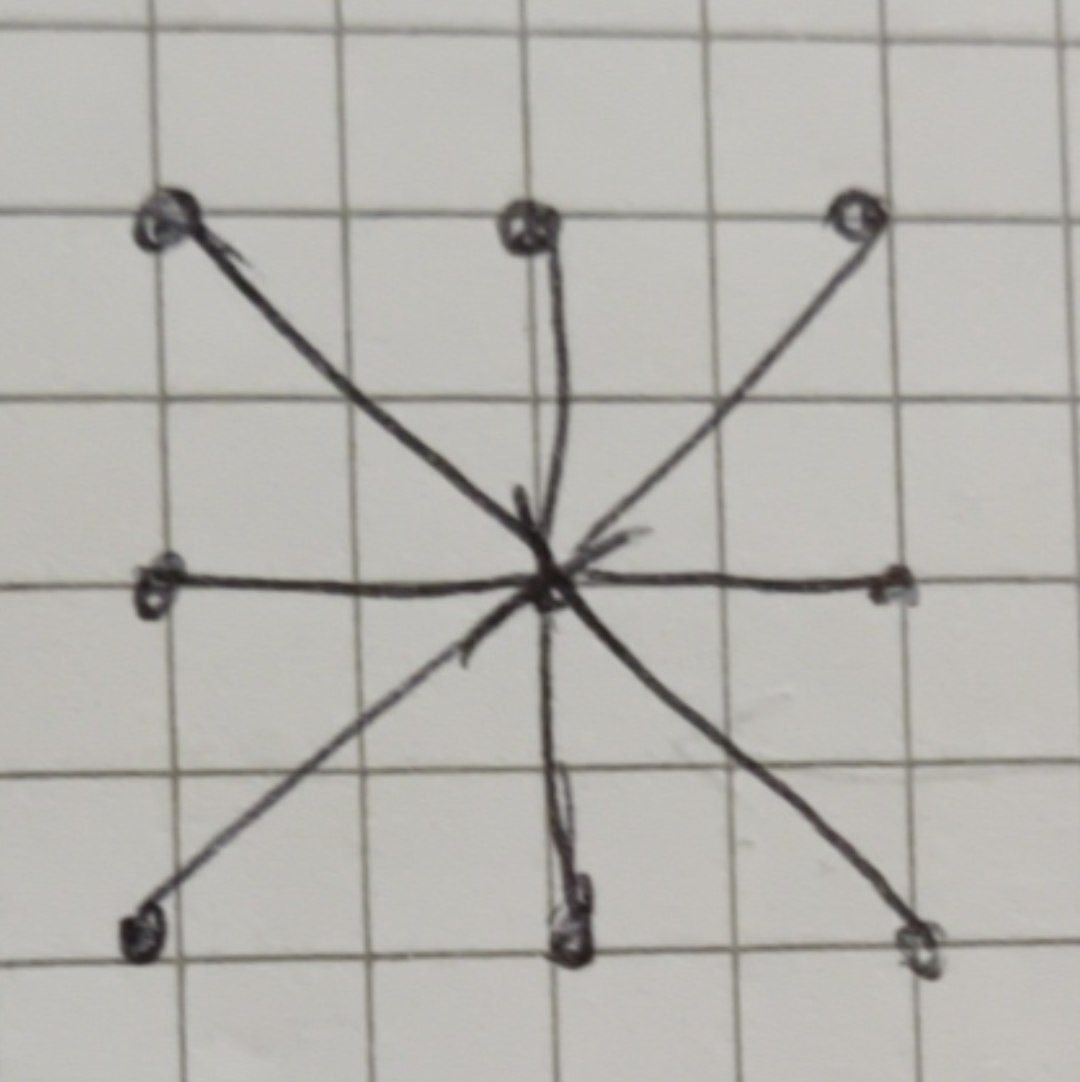
\includegraphics[width=0.35\linewidth]{img/reticoloLez8.png}
                \label{reticoloLez8}
            \end{figure}

            Si connette il centro con i punti reticolari vicini: se per ogni segmento si considera un piano ortogonale ad esso, che passa per i punti medi del segmento, in due dimensioni vengono individuate delle aree che in tre dimensioni corrispondono a dei volumi:
            \begin{figure}[h!]
                \centering
                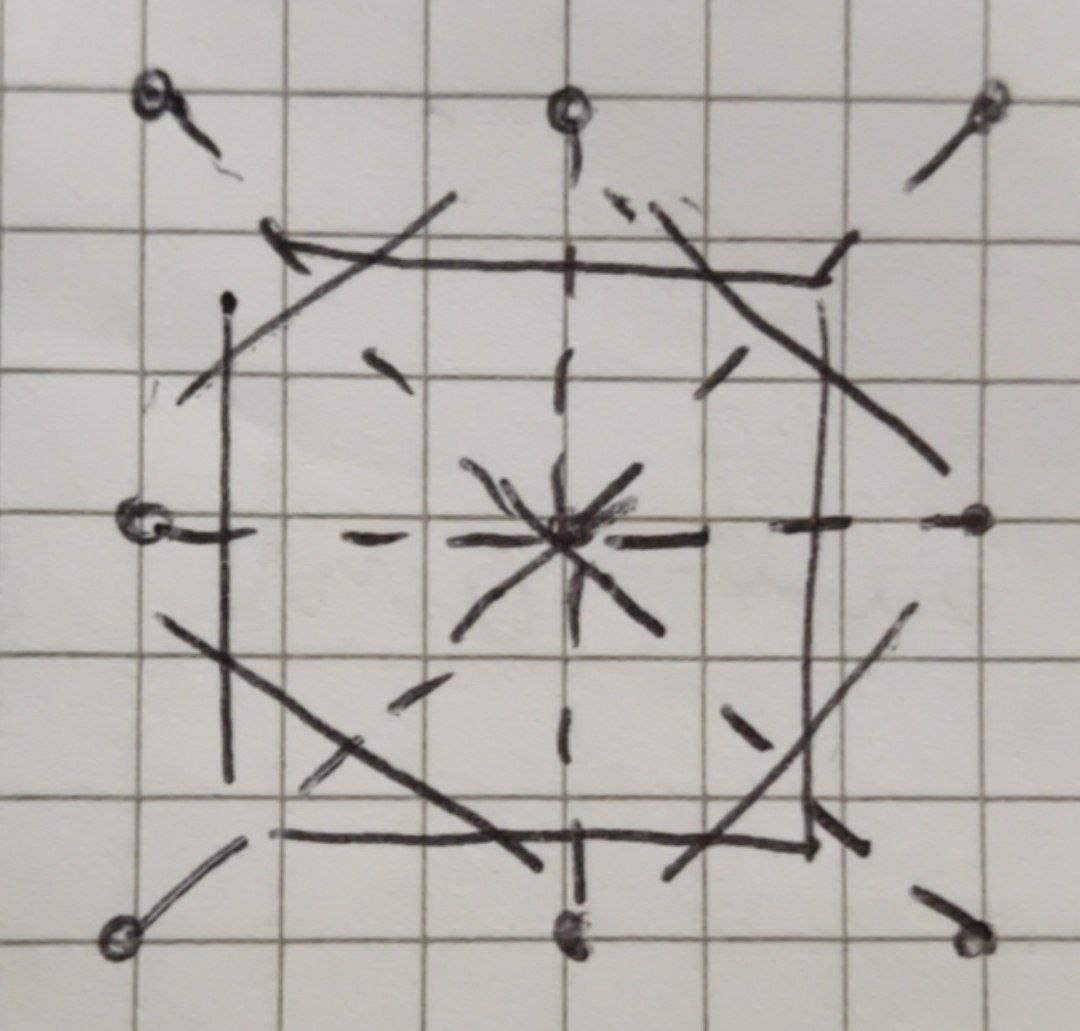
\includegraphics[width=0.35\linewidth]{img/reticolo2Lez8.png}
                \label{fig:enter-label}
            \end{figure}
        \paragraph{}
            Il più piccolo volume individuato che racchiude il punto reticolare di riferimento è detto \textbf{cella di Wigner-Seitz}. Nel caso del reticolo quadrato la cella di Wigner-Seitz è una cella elementare quadrata, dunque la differenza non si nota. È più evidente se per esempio si considera una cella romboidale in 3D:
            \begin{figure}[h!]
                \centering
                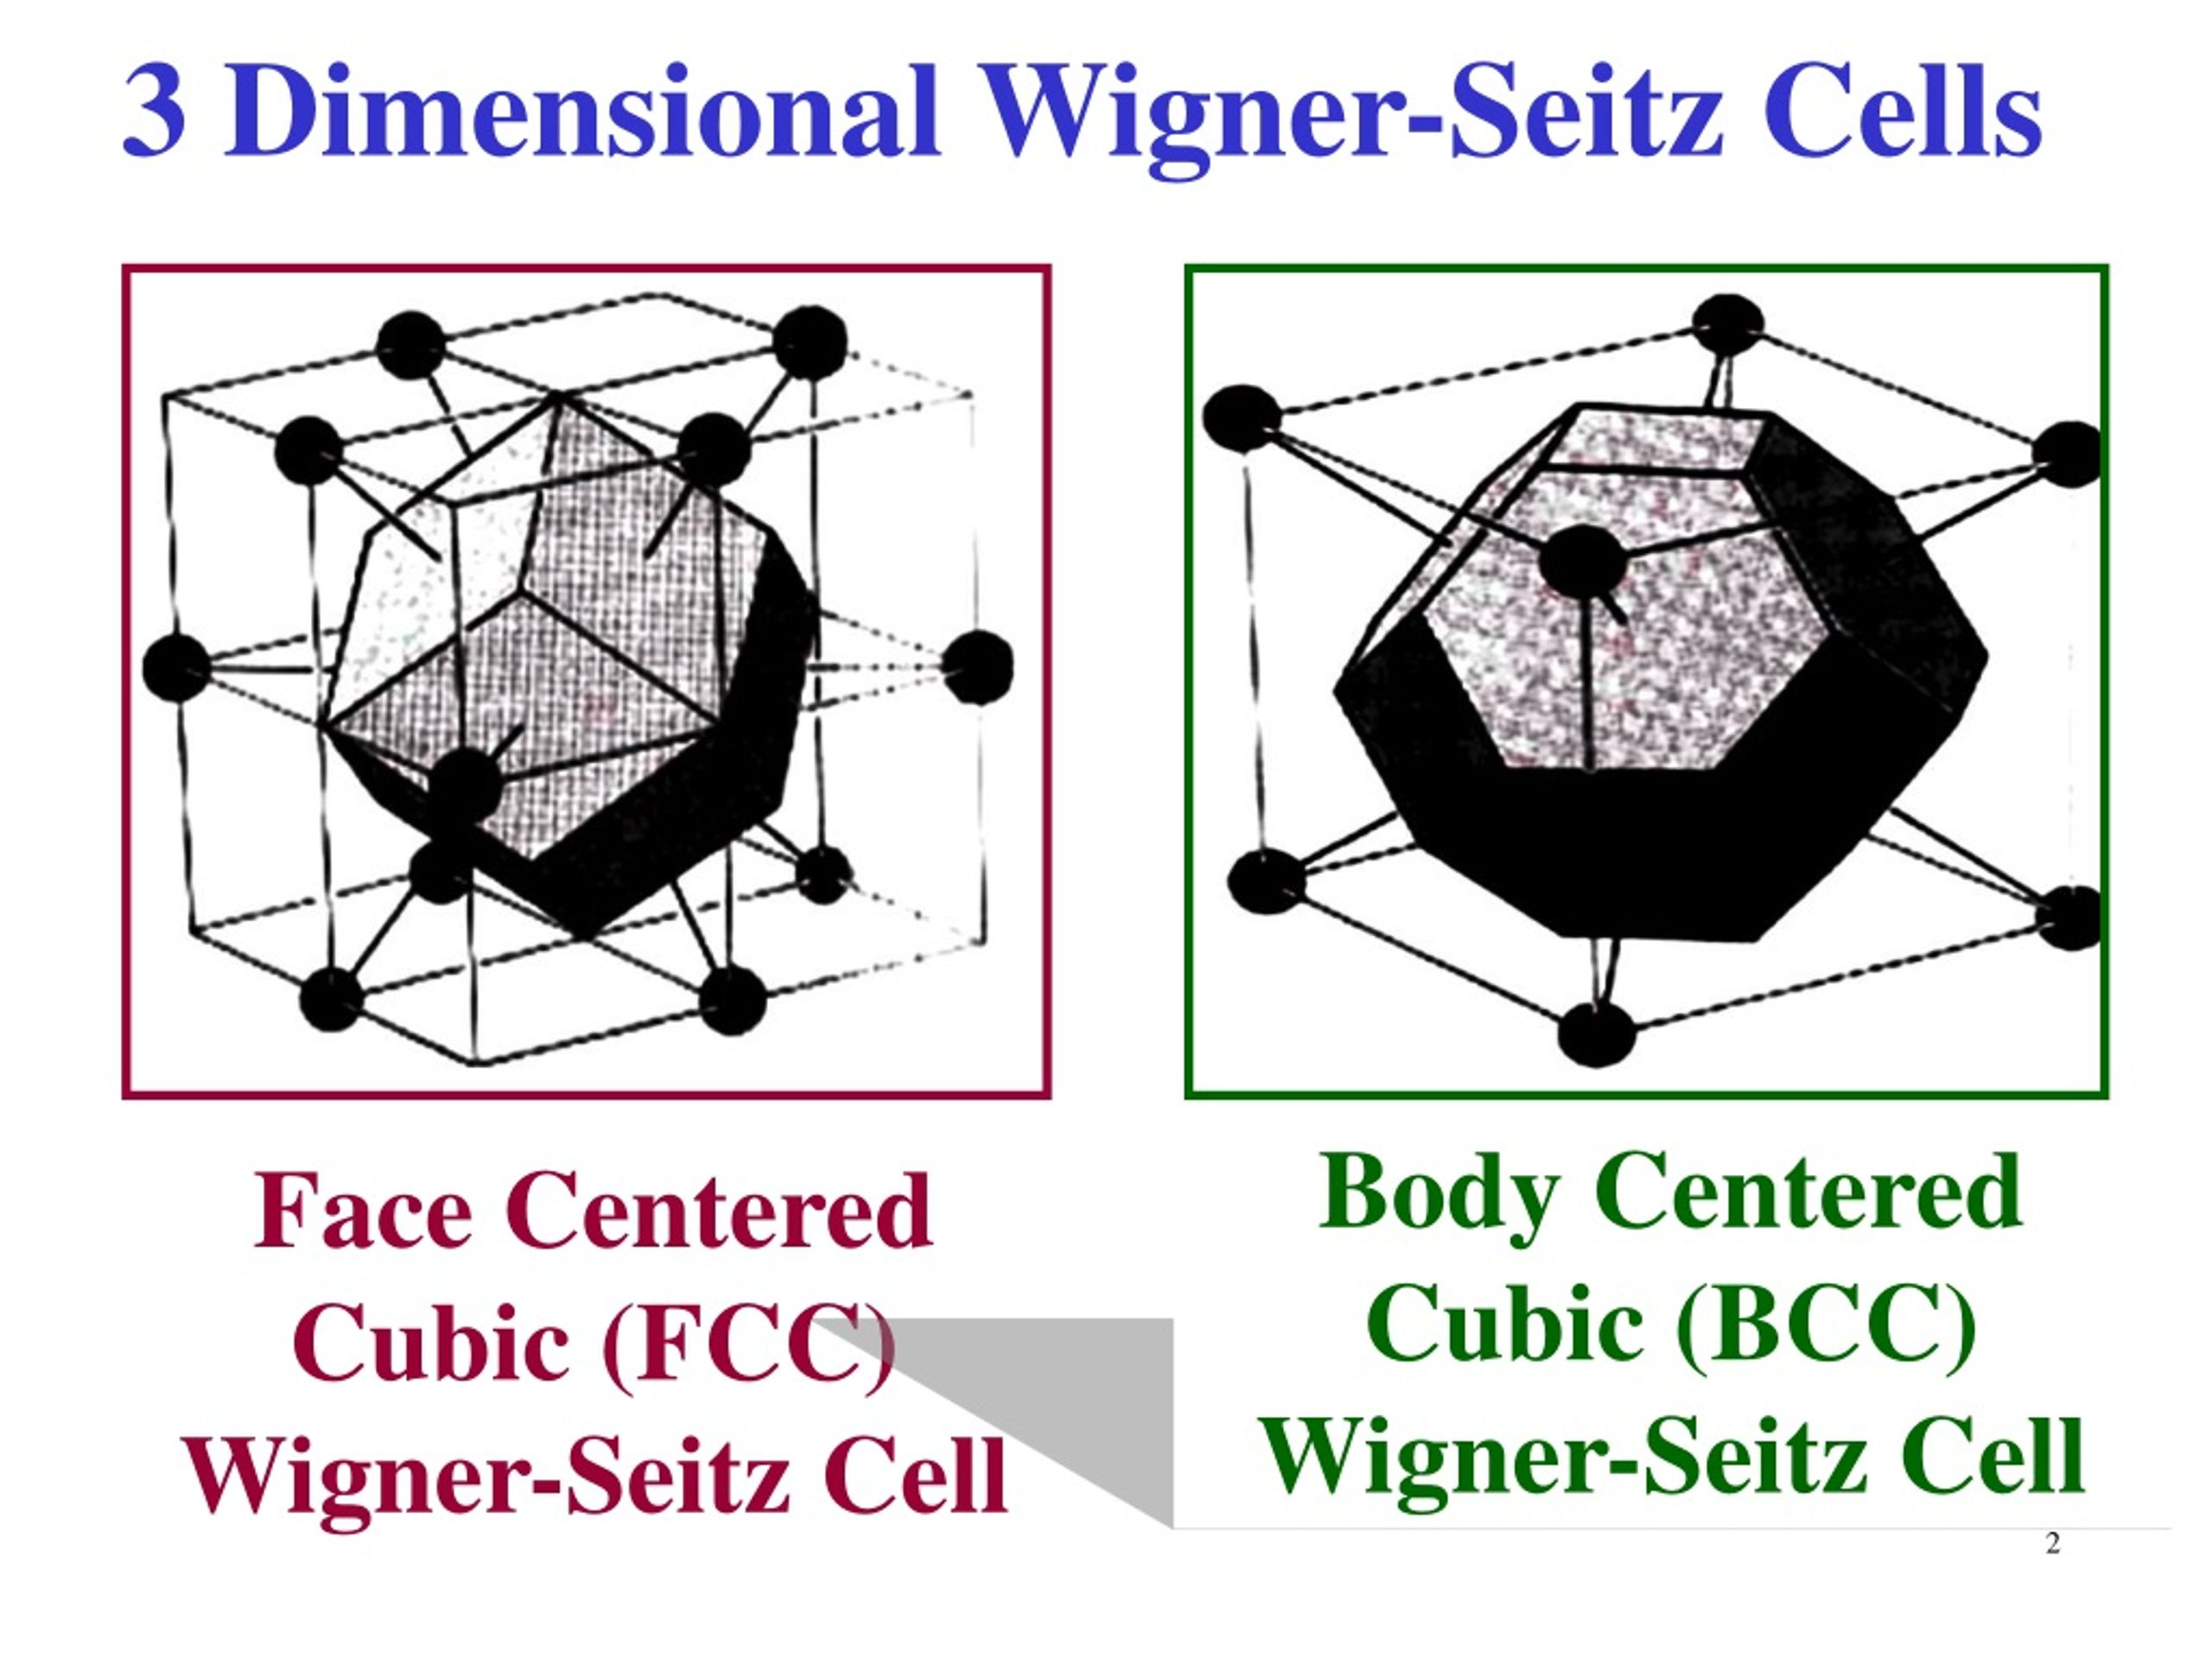
\includegraphics[width=0.35\linewidth]{img/WignerSeitzLez8.png}
                \label{wignerSeitzLez8}
            \end{figure}
            La \textbf{zona di Brillouin} è semplicemente la zona di Weigner-Seitz del reticolo reciproco

        \section{Diffrazione a raggi X da parte di un cristallo}
        \paragraph{}
            In un reticolo cristallino, ogni zona fra un punto reticolare ed un altro, quando questo viene investito da un'onda elettromagnetica, si comporta da sorgente d'onda. Ricordiamo che per trattare la luce come corpuscolo sottoforma di raggi, e non come onde, le dimensioni delle fessure tra un punto reticolare e l'altro devono essere molto maggiori rispetto alla lunghezza d'onda $\lambda$. 
            \begin{figure}[h!]
                \centering
                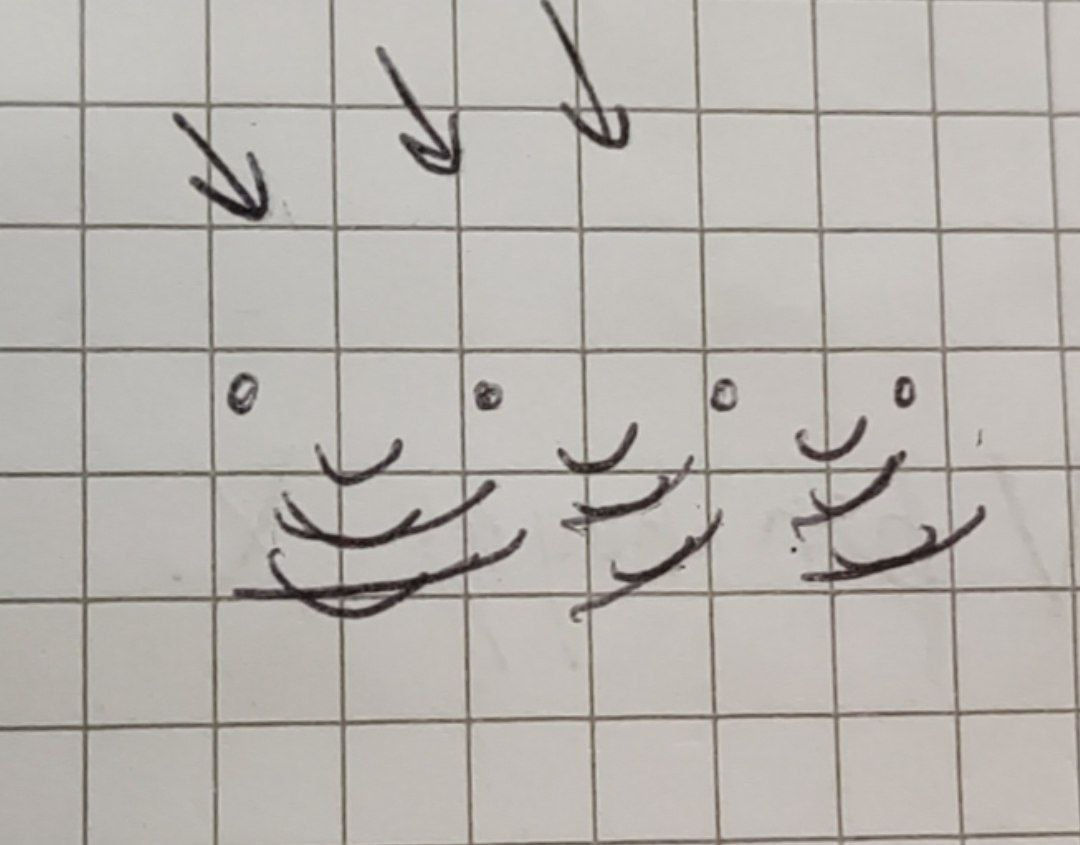
\includegraphics[width=0.5\linewidth]{img/diffrazioneLez8.png}
            \end{figure}
        \paragraph{}
            La distanza media fra un atomo ed un altro è nell'ordine di qualche \si{\angstrom}, dunque la lunghezza d'onda dei raggi della luce che bisogna utilizzare per trattare il fenomeno in modo corpuscolare è quella dei raggi X, $\lambda \simeq 0.1 \div 10 $\r{A}. Per produrre i raggi X si può utilizzare, per esempio, un tubo catodico:
            \begin{figure}[h!]
                \centering
                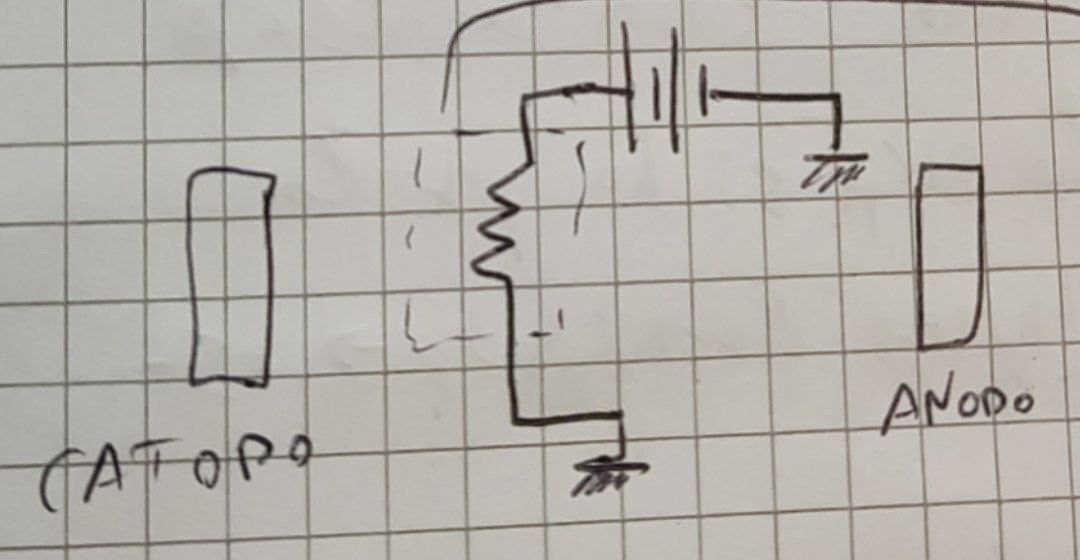
\includegraphics[width=0.85\linewidth]{img/tuboCatodicoLez8.png}
            \end{figure}
            Si scalda un filamento metallico di una certa lega, applicando ai suoi capi un'elevata d.d.p. Per effetto termoionico vengono emessi elettroni, che vengono accelerati con una coppia di elettrodi con potenziale $\Delta V$. Allora gli elettroni impattano l'anodo con energia $E_{k}=c \Delta V$ che viene trasferita agli elettroni dell'anodo che di tutta risposta salgono di livello energetico:
            \begin{figure}[h!]
                \centering
                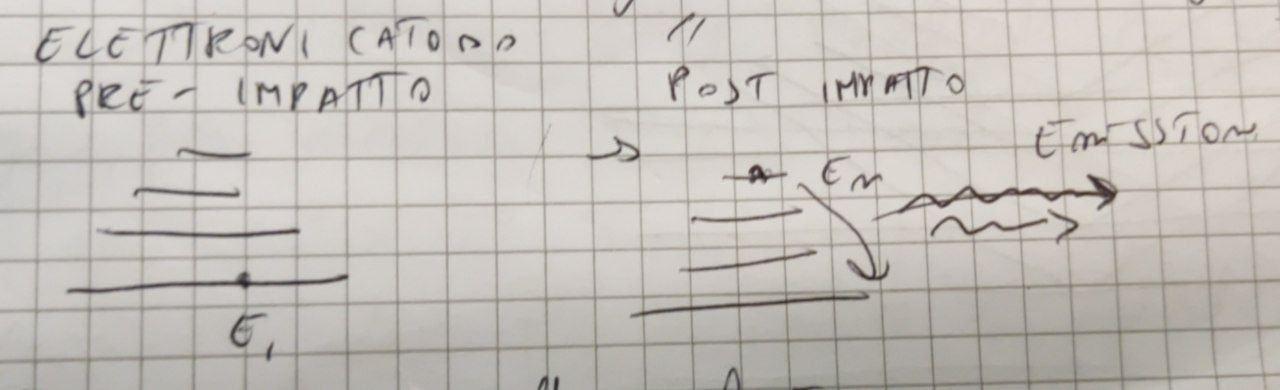
\includegraphics[width=0.85\linewidth]{img/elettroniSaltoLez8.png}
                \label{fig:enter-label}
            \end{figure}
            Una volta che questi scendono al livello energetico inferiore, emettono fotoni X.
            Affinché siano fotoni X, occorre che $$\lambda = \displaystyle \frac{c}{\nu} = \frac{c h}{\Delta E} = \lambda_{X} = \frac{1.24nm}{\Delta E[keV]} \implies \Delta E \sim 1 \div 10 keV$$
            \newpage
            \paragraph{}
                Il tipico spettro di emissione è fatto così:
                \begin{figure}[h!]
                    \centering
                    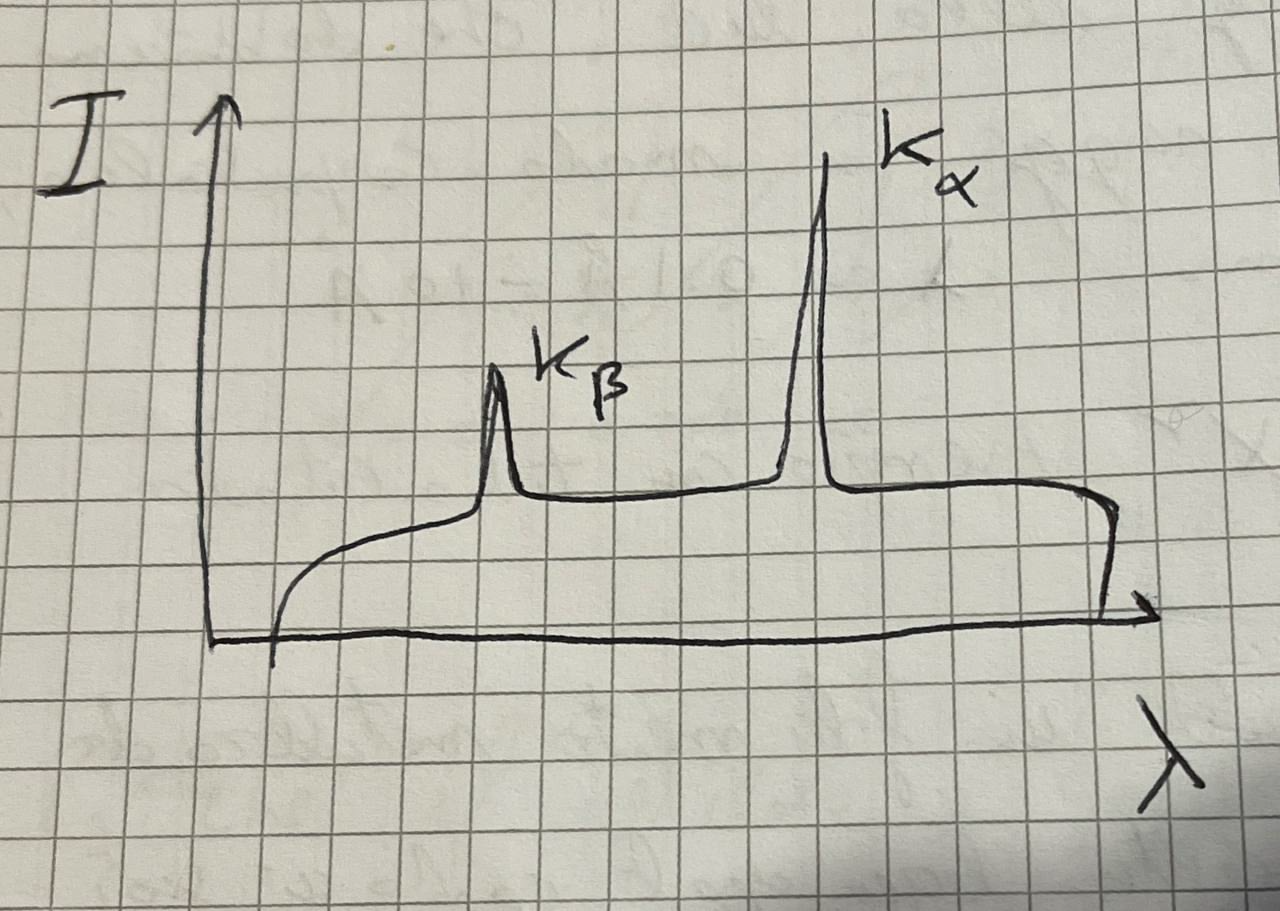
\includegraphics[width=0.5\linewidth]{img/spettroEmissioneLez8.png}
                \end{figure}
                dove con $I$ si indica l'intensità luminosa.\newline
                Per il rame, ad esempio, per $\lambda = k_{\alpha}$, che è la lunghezza d'onda dei fotoni emessi durante la transizione $2p \to 1s$, $k_{\alpha}=1.54 $\r{A}, mentre $\lambda = k_{b}$ è quella corrispondente alla transizione $3p \to 1s$.

            \paragraph{Diffrazione secondo Bragg}: la questione viene trattata dal punto di vista \textit{geometrico}. Considerato il cristallo come un insieme di piano reticolari paralleli, Bragg assunse che le radiazioni venissero riflesse specularmente, dunque con lo stesso angolo di incidenza $\theta$ rispetto al piano del reticolo.
            \begin{figure}[h!]
                \centering
                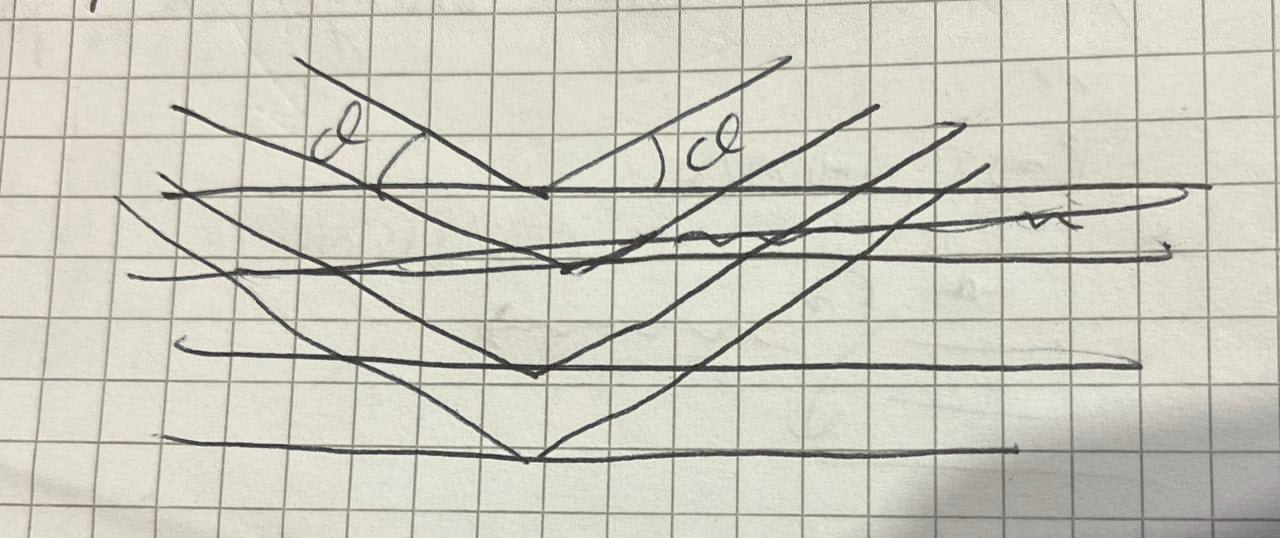
\includegraphics[width=0.75\linewidth]{img/reticoloBragg1Lez8.png}
            \end{figure}

            \paragraph{}
                I raggi, di luce monocromatica a raggi X, vengono specchiati e si incrontrano all'infinito. Come sappiamo l'interferenza può essere costruttiva o distruttiva: il criterio con cui le onde riflesse del cristallo hanno diffrazione costruttiva o distruttiva è la differenza di cammino fra queste.
                    \begin{figure}[h!]
                        \centering
                        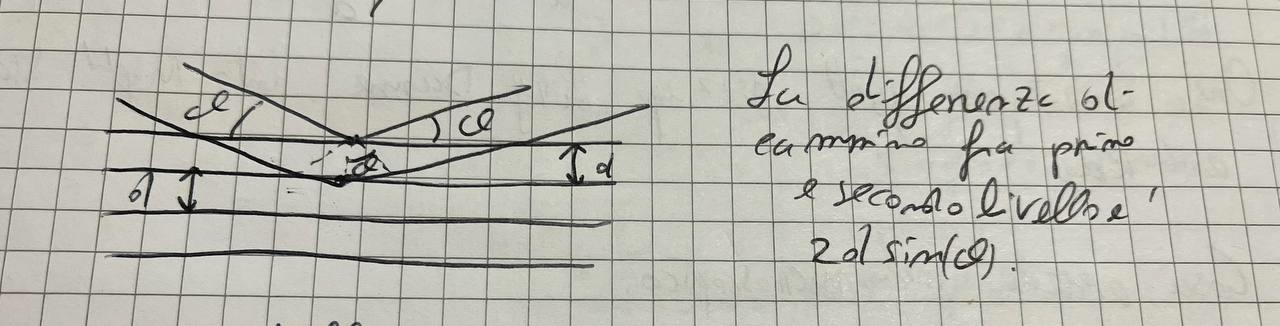
\includegraphics[width=0.75\linewidth]{img/diffCamminoLez8.png}
                       
                    \end{figure}
            \newline
            La differenza di cammino fra primo e secondo livello è $2d\sin(\vartheta)$.
            \newpage
            Dunque per avere diffrazione costruttiva, poiché la condizione è che le onde arrivino in fase (i.e. con differenza di fase nulla), deve risultare:
            $$2d\sin{(\vartheta)} = n \lambda \qquad \qquad n \in \mathbb{N}$$
            dette \textbf{condizioni di diffrazione di Bragg}.

            \paragraph{}
                Le condizioni di Bragg possono essere sfruttate per ricavare la distanza $d$ tra i piani reticolari, ricavando sperimentalmente valori di $\vartheta$ tali per cui la condizione è soddisfatta.\newline
                L'esperimento che viene condotto per fare quanto detto è il "$\vartheta-2\vartheta$". 
                \begin{figure}[h!]
                    \centering
                    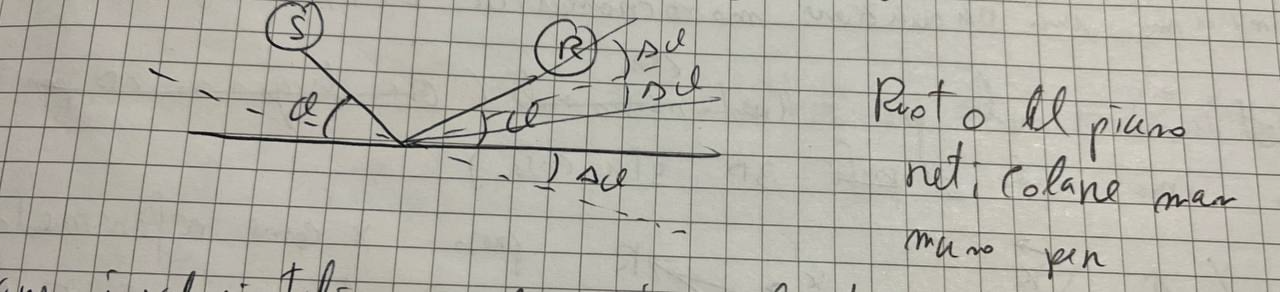
\includegraphics[width=0.85\linewidth]{img/theta2thetaLez8.png}
                \end{figure}

                \paragraph{}
                    L'apparato è composto da una sorgente di raggi X $S$ ed un rivelatore $R$, che in virtù dell'assunzione di cristallo spazialmente infinito è posto molto lontano rispetto al piano del cristallo.\newline
                    La sorgente $S$ di raggi X è di solito difficile da ruotare, quindi quello che si fa per variare i valori di $\vartheta$ è ruotare il piano reticolare di $\vartheta$ ed il rivelatore di $2 \vartheta$, perché $\vartheta$ è l'angolo necessario di rotazione per seguire l'apparato e un ulteriore $\vartheta$ per far in modo che l'angolo rimanga riflesso specularmente rispetto al piano reticolare verso il rivelatore.

                    \paragraph{}
                        Ruotando l'apparato di $\Delta \vartheta$ (da qui in poi quest'espressione corrisponderà alla rotazione del piano di $\Delta \vartheta$ e del rivelatore di $2 \Delta \vartheta$), il nuovo angolo candidato a soddisfare le condizioni di Bragg è:
                        $$\vartheta ' = \vartheta - \Delta \vartheta$$
                    \paragraph{}
                        Nel caso di un reticolo ortorombico si può dimostrare che per il piano $h,k,l$ risulta:
                        $$\frac{1}{d^{2}} = \frac{h^{2}}{a^{2}}+\frac{k^{2}}{b^{2}}+\frac{l^{2}}{c^{2}}$$
                        che si riduce nel caso di reticolo cubico:
                        $$\frac{1}{d^{2}} = \frac{h^{2}+k^{2}+l^{2}}{a^{2}}$$


        \section{Fenomeni di scattering nel microscopico}
            \paragraph{}
                Un atomo generico del reticolo è identificato nello spazio dal vettore:
                $$\vec{r} = n_{1}\vec{a}+n_{2}\vec{b}+n_{3}\vec{c}$$
                Limitiamoci al caso semplice di un reticolo monoatomico con un solo atomo per punto reticolare. Il reticolo viene investito da una radiazione monocromatica $\vec{E}(\vec{r},t) = \vec{E}_{0}e^{i(\vec{k}\cdot \vec{r}-\omega t)}$.Nel piano tridimensionale (disegnato in 2D per semplicità di rappresentazione), preso il punto reticolare segnato con una 'x' in figura come riferimento, la sua posizione rispetto all'origine è identificata da $\vec{r}$ mentre quella del rivelatore da $\vec{R}$. La posizione del rivelatore \textit{rispetto al punto reticolare di riferimento} è descritta da $\vec{\rho} = \vec{R}- \vec{r}$:
                \begin{figure}[h!]
                    \centering
                    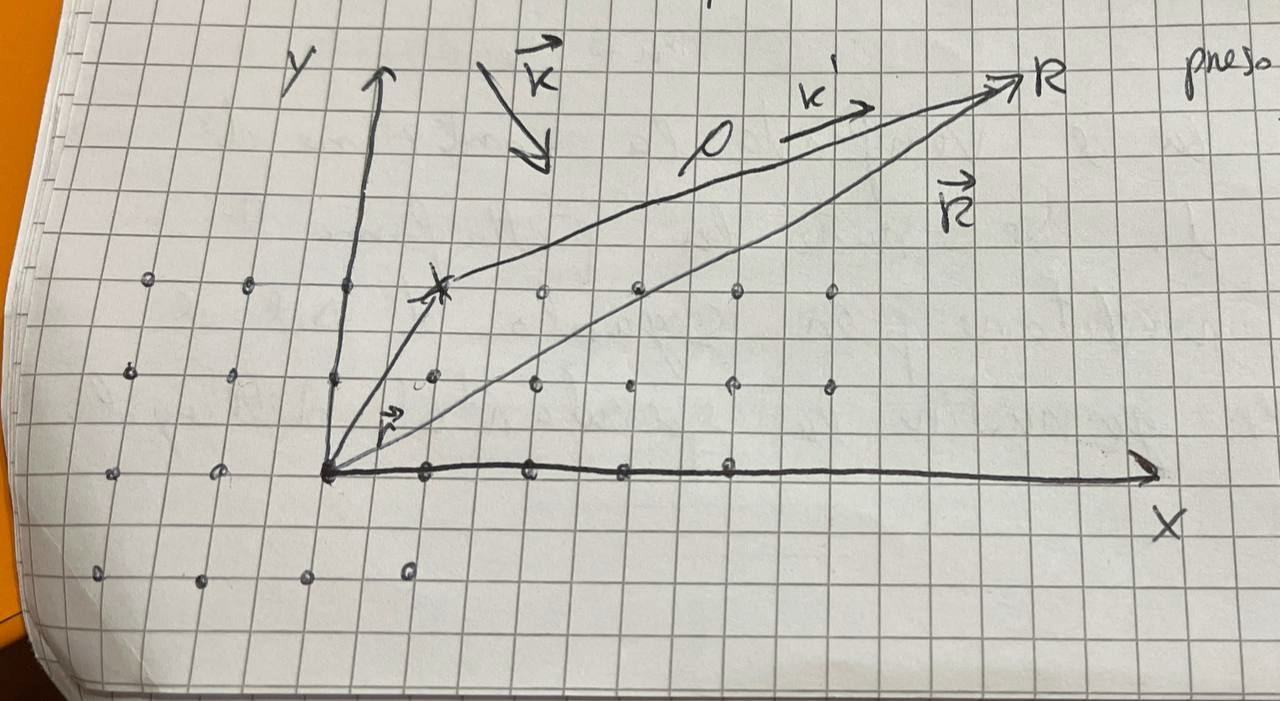
\includegraphics[width=0.85\linewidth]{img/scatteringLez8.png}
                \end{figure}

                \paragraph{}
                    Gli atomi in questa situazione qua, come detto sopra, sono considerabili centri di diffusione delle radiazioni. Assumiamo che lo scattering (letteralmente "diffusione" in inglese ndr) sia puramente \textbf{elastico}: il fotone arriva, viene assorbito e viene rimbalzato fuori \textbf{con la stessa energia}. In virtù del fatto che l'energia rimane la stessa, eguagliandone i valori pre e post-urto:
                    $$\hbar \nu = \hbar \nu ' \implies \omega ' = \omega \implies |k| = |k'|$$
                    Nel caso ci fosse bisogno di ricordare la relazione fra $\omega$ e $k$, le prime lezioni potrebbero essere illuminanti.

                \paragraph{}
                    Dunque per urti elastici \textbf{il modulo} del vettore d'onda di conserva, ma ovviamente la direzione è diversa. Il campo originato dallo scattering $\vec{E}_{sc}$ è esprimibile come:
                    $$\vec{E}_{sc} = f\vec{E}(\vec{r},t)\frac{\exp({i \vec{k}' \cdot \vec{\rho}})}{\rho}$$

                    Notiamo varie cose: 
                    \begin{itemize}
                        \item  L'espressione fa riferimento al campo originato da un singolo atomo (i.e. singolo centro di diffusione).
                        \item Il termine $\displaystyle \frac{\exp{(i (\vec{k}' \cdot \vec{\rho}}))}{\rho}$ è l'espressione classica di un'onda E.M. sferica.
                        \item Il termine $f$ è detto \textit{fattore di struttura atomico} ed è generalmente complesso. Se ne parlerà nelle prossime lezioni.
                    \end{itemize} 

                \paragraph{}Esplodendo l'espressione del campo $\vec{E}(\vec{r},t)$ si ottiene:
                $$\vec{E}_{sc} = f \vec{E}_{0} \frac{1}{\rho} \exp{(i(\vec{k} \cdot \vec{r} + \vec{k}' \cdot \vec{\rho}) - \omega t)}$$
                Manipoliamo il termine:
                $$\vec{k} \cdot \vec{r} + \vec{k'} \cdot \vec{\rho} = \vec{k} \cdot \vec{r} + \vec{k'} \cdot (\vec{R}-\vec{r}) = \vec{k'} \cdot \vec{R} + (\vec{k}-\vec{k'})\vec{r}$$
                $$ = \vec{k'} \cdot \vec{R}-\Delta \vec{k} \cdot \vec{r}$$
                dove $\Delta \vec{k} = \vec{k'}-\vec{k}$.

                \paragraph{}
                    Il rivelatore è a grande distanza dunque $\vec{\rho}$ ed $\vec{R}$ sono praticamente paralleli, per cui il prodotto interno si può approssimare al prodotto dei moduli:
                    $\vec{k'} \cdot \vec{R} \simeq k' \cdot \vec{R} = k R$
                    e dunque:
                    $$\vec{k'} \cdot \vec{r}+ \vec{k'} \cdot \vec{\rho} \simeq kR - \Delta \vec{k} \cdot \vec{r}$$
                \paragraph{}
                    Poiché a grande distanza $\rho \simeq R$, l'onda sferica diffusa dal singolo atomo è:
                    $$\vec{E}_{sc} = \vec{E}_{0} \frac{e^{i(kR - \omega t)}}{R} f e^{-i \Delta \vec{k} \cdot \vec{r}}$$.

                    Il termine esponenziale $fe^{-i\Delta \vec{k} \cdot \vec{r}}$ evidenzia la dipendenza del campo di scattering dalle caratteristiche atomiche del reticolo, che in questo caso è composto da atomi uguali (i.e. fattori di struttura uguali).
                \paragraph{}
                    Guardiamo ora al reticolo in toto. Il numero di atomi lungo le tre direzioni spaziali è rispettivamente $N_{1}, N_{2}$ ed $N_{3}$.
                    Dunque se $\vec{r} = n_{1}\vec{a}+n_{2}\vec{b}+n_{3}\vec{c}$, allora:
                    $$n_{1} \in [0, N_{1}-1]$$
                    $$n_{2} \in [0, N_{2}-1]$$
                    $$n_{3} \in [0, N_{3}-1]$$
                    Sommando su tutti gli atomi si ricava il \textbf{campo di scattering totale}:
                    $$\vec{E}_{sc, tot} = \vec{E}_{0} \frac{e^{i(kR-\omega t)}}{R} f \sum_{n_{1} = 0} ^{N_{1} -1}\exp{(-in_{1}\Delta\vec{k} \cdot \vec{a})}\sum_{n_{2} = 0} ^{N_{2} -1}\exp{(-in_{2}\Delta\vec{k} \cdot \vec{b})}\sum_{n_{3} = 0} ^{N_{3} -1}\exp{(-in_{3}\Delta\vec{k} \cdot \vec{c})}$$
                \newpage
                \paragraph{}
                    Statisticamente tutte e tre quelle sommatorie sono nulle \textbf{tranne} in un caso, cioè quello nel quale gli esponenti sono multipli interi di $2\pi$, il che equivale a dire che nel caso in cui risulti:
                    $$\Delta \vec{k} \cdot \vec{a} = 2 \pi h$$
                    $$\Delta \vec{k} \cdot \vec{b} = 2 \pi k$$
                    $$\Delta \vec{k} \cdot \vec{c} = 2 \pi l$$
                    allora il campo di scattering totale vale:
                    $$\vec{E}_{sc, tot} = \vec{E}_{0}\frac{e^{i(kR - \omega t)}}{R} f N_{1}N_{2}N_{3}$$

                    \paragraph{}
                    Questo significa che i massimi di diffrazione del cristallo si trovano per valori $\vec{k} = (h, k, l)$,  ovvero per terne di indici di Miller: ciò equivale a dire che $\Delta \vec{k}$ deve essere un vettore del reticolo reciproco. Tale requisito prende il nome di \textbf{Condizioni di Von Laue}.

                    \paragraph{}
                        Le condizioni di Bragg e von Laue sono equivalenti. Se vale von Laue infatti, valutando il valore:
                        $$|\Delta k| ^{2} = A^{2}h^{2}+C^{2}k^{2}+C^{2}l^{2} = (2\pi)^{2} (\frac{h^{2}}{a^{2}}+\frac{k^{2}}{b^{2}}+\frac{l^{2}}{c^{2}}) = (\frac{2 \pi}{d})^{2}$$
                        da cui risulta che $d$ è multiplo intero della funzione d'onda (basta tener conto che il modulo del vettore d'onda è pari a $|k| 0 \frac{2\pi}{\lambda}$

    \section{Fattori di struttura nella diffrazione a Raggi X}
        \paragraph{} La big ass espressione con le tre sommatorie:
        $$Q = \sum_{n_{1} = 0} ^{N_{1} -1}\exp{(-in_{1}\Delta\vec{k} \cdot \vec{a})}\sum_{n_{2} = 0} ^{N_{2} -1}\exp{(-in_{2}\Delta\vec{k} \cdot \vec{b})}\sum_{n_{3} = 0} ^{N_{3} -1}\exp{(-in_{3}\Delta\vec{k} \cdot \vec{c})}$$
        prende il nome di $Q$, fattore di struttura \textbf{del reticolo}, perché dipende solo dalla geometria del cristallo.

        \paragraph{} Analizziamo ora cosa succede nel caso di un reticolo composto da atomi diversi e con più atomi per punto reticolare. In questo caso, bisogna tener conto della posizione dell'atomo all'interno della cella, modificando il vettore posizione come segue:
        $\vec{r}_{atomo} = \vec{r}+r_{j}$
        dove $\vec{r}$ è la posizione del punto reticolare di riferimento della cella ed $r_{j}$ la posizione dell'atomo all'interno della cella \textit{rispetto} al punto reticolare di riferimento. Visto in questo modo, i due vettori sono descritti da:
       $$ \begin{cases}
            \vec{r} = n_{1}\vec{a}+n_{2}\vec{b}+n_{3}\vec{c} \\
            \vec{r}_{j} = x_{j}\vec{a}+y_{j}\vec{b}+z_{j}\vec{c}
         \end{cases}$$
         dove $n_{1},n_{2},n_{3} \in N$ ed $x_{j},y_{j},z_{j}$ sono generalmente non interi.
        \paragraph{}
            A fronte di questa variazione, l'espressione del campo di scattering generato dal $j$-esimo atomo della cella di posizione $\vec{r}$ del reticolo è dato da:
            $$\vec{E}_{sc} = \vec{E}_{0}\frac{e^{i(kR-\omega t)}}{R}f_{j}$$

         dove $f_{j}$ è il fattore atomico relativo al $j$-esimo atomo.

        \paragraph{}
            Tenendo conto del fatto che in una cella ci sono massimo una decina di atomi, allora $j$ è circa al massimo dieci. Allora il campo scatterato totale è dato da:
            $$\vec{E}_{sc, tot} = \vec{E}_{0} \frac{e^{i(kR - \omega t)}}{R} \sum_{n_{1},n_{2},n_{3}} ^{N_{1},N_{2},N_{3}} e^{i \vec{r} \cdot \Delta \vec{k}} \sum_{j} f_{j} e^{-i \vec{r}_{j} \cdot \Delta \vec{k}} = \vec{E}_{0}\frac{e^{i(kR-\omega t)}}{R} Q \delta$$
            dove $\delta = \sum_{i} f_{j}e^{-i\vec{r}_{j}\cdot \Delta k}$ è detto \textbf{fattore di struttura della base atomica}. Poiché affinché il $Q$ non sia nullo deve valere $\Delta \vec{k} = \vec{G}$, nel dettaglio $\delta$ con $s$ atomi per cella si esprime come:
            $$\delta = \sum_{j=1} ^{s} f_{j}e^{-i2\pi(hx_{j}+ky_{j}+lz_{j})}$$

        \paragraph{Esempio con reticolo cubico BCC monoatomico}
            Alla cella cubica BCC sono associati due atomi indipendenti. Allora se il primo atomo indipendente, scelto arbitrariamente fra i nove, ha coordinate $\vec{r}_{1}=(0,0,0)$, il secondo indipendente scelto sarà $\vec{r}_{2} = (\frac{1}{2}, \frac{1}{2}, \frac{1}{2})$, perché non esiste una combinazione lineare di numeri interi per passare da $\vec{r}_{1}$ ad $\vec{r}_{2}$. Il fattore di struttura atomico è lo stesso e quindi:
            $$\delta = f(e^{(-i r_{2} \cdot \vec{G})}+e^{-i(\vec{r}_{2} \cdot \vec{G})} = f(1+e^{-i\pi(h+k+l)})$$.
        \paragraph{}
            Se $h+k+l$ è dispari $\delta = 0$, altrimenti $\delta = 2f$.

        \paragraph{}
            Nell'atomo sono gli elettroni che permettono la diffusione della radiazione. Consideriamo allora una versione ulteriormente espansa del vettore posizione:
            $$\vec{r}_{elettrone} = \vec{r} + \vec{r}_{j} + \vec{r}'$$
            dove $\vec{r'}$ tiene conto della "posizione" dell'elettrone, cioè è un certo vettore che traccia la presenza o meno dell'elettrone all'interno di un orbitale.
            Sia $\rho(\vec{r})$ una certa funzione densità di probabilità (da verificare ndr), per l'elettrone non ha senso sommare ma bisogna integrare tale funzione di densità di probabilità nella zona dell'orbitale dove ci si aspetta di trovare l'elettrone e dunque risulta:
            $$\vec{E}_{sc, tot} = \vec{E}_{0} \frac{e^{i(kR - \omega t)}}{R} \sum_{n_{1}, n_{2}, n_{2}} \cdots \sum_{j=1} ^{s} \cdots \int \gamma \rho (\vec{r'}) e^{-i \Delta \vec{k}(\vec{r}+\vec{r}_{j}+\vec{r'})}dV$$
            dove $\gamma$ è il termine asimmetrico al terz'ordine dello sviluppo dell'energia potenziale della buca di potenziale che abbiamo ricavato qualche lezione fa'.
        \paragraph{}
            Fattorizzando ulteriormente:
            $$\vec{E}_{sc,tot} = \frac{e^{i(k R - \omega t)}}{R} Q \sum_{j =1} \sum_{j=1} ^{s} e^{-iG \cdot \Delta \vec{r}_{j}} \gamma \int \rho_{j} (\vec{r}) e^{-i\vec{G} \cdot \vec{r'}} dV_{j}$$
            dove $f_{j} = \gamma \int \rho_{j} (\vec{r}) e^{-i\vec{G} \cdot \vec{r'}}dV_{j}$

            Ci sono due cose interessanti da dire sul fattore $f_{j}$: il primo è che sperimentalmente si verifica che $f_{j} \propto Z_{j}$, cioè che sia proporzionale al numero atomico. La seconda è che la dipendenza da $\vec{G}$ suggerisce che al variare del piano di riflessione considerato, in quanto $\vec{G}$ è un vettore del reticolo reciproco, varia anche il fattore di struttura.

        \paragraph{La dipendenza dalla temperatura} Ciò che abbiamo appena detto vale a temperatura nulla e, seppur sia valido mediamente per temperature non nulle, pecca di imprecisione. Introduciamo allora un fattore correttivo $u(t)$ che descrive in che modo l'atomo si sposta all'interno della cella nel corso del tempo:
        $$\vec{r}_{atomo} = \vec{r} + [\vec{r}_{j} + u(t)]+\vec{r'}$$

        \paragraph{}
        Le tipiche energie di agitazione termiche sono dell'ordine di $k_{b}T \simeq \frac{1}{40}eV$.
        Questo ha effetto sul fattore di struttura del reticolo, il quale dipende dalla geometria dello stesso:
        $$Q_{j} = Q_{0}\exp{(-\frac{G^{2}k_{b}T}{2\beta_{j} ^{2}})}$$
        dove $Q_{0}$ è il valore di $Q$ a temperatura nulla e $\beta_{j}$ il coefficiente elastico ricavato durante la trattazione della buca di potenziale. Esso può essere scritto come
        $$\beta^{2} = M_{j}\omega_{j} ^{2}$$
        cioè come il prodotto fra la massa e il quadrato della frequenza delle oscillazioni dell'atomo $j$-esimo.

        \paragraph{}
            Cosa succede se per effetto della tempertura ci si sposta da un valore di $\vartheta$, per il quale c'è un massimo, ad un valore $\vartheta + \varepsilon$? \newline
            L'intensità della radiazione riflessa $I$ sarà funzione di un certo parametro
            $$x = 2 \frac{\pi \varepsilon L_{x} \cos{(\vartheta)}}{\lambda}$$
            \newpage
            Non c'interessa cos'è $\lambda$ per i nostri fini, mentre $L_{x}$ è l'estensione del cristallo.La situazione è questa:
            \begin{figure}[h!]
                \centering
                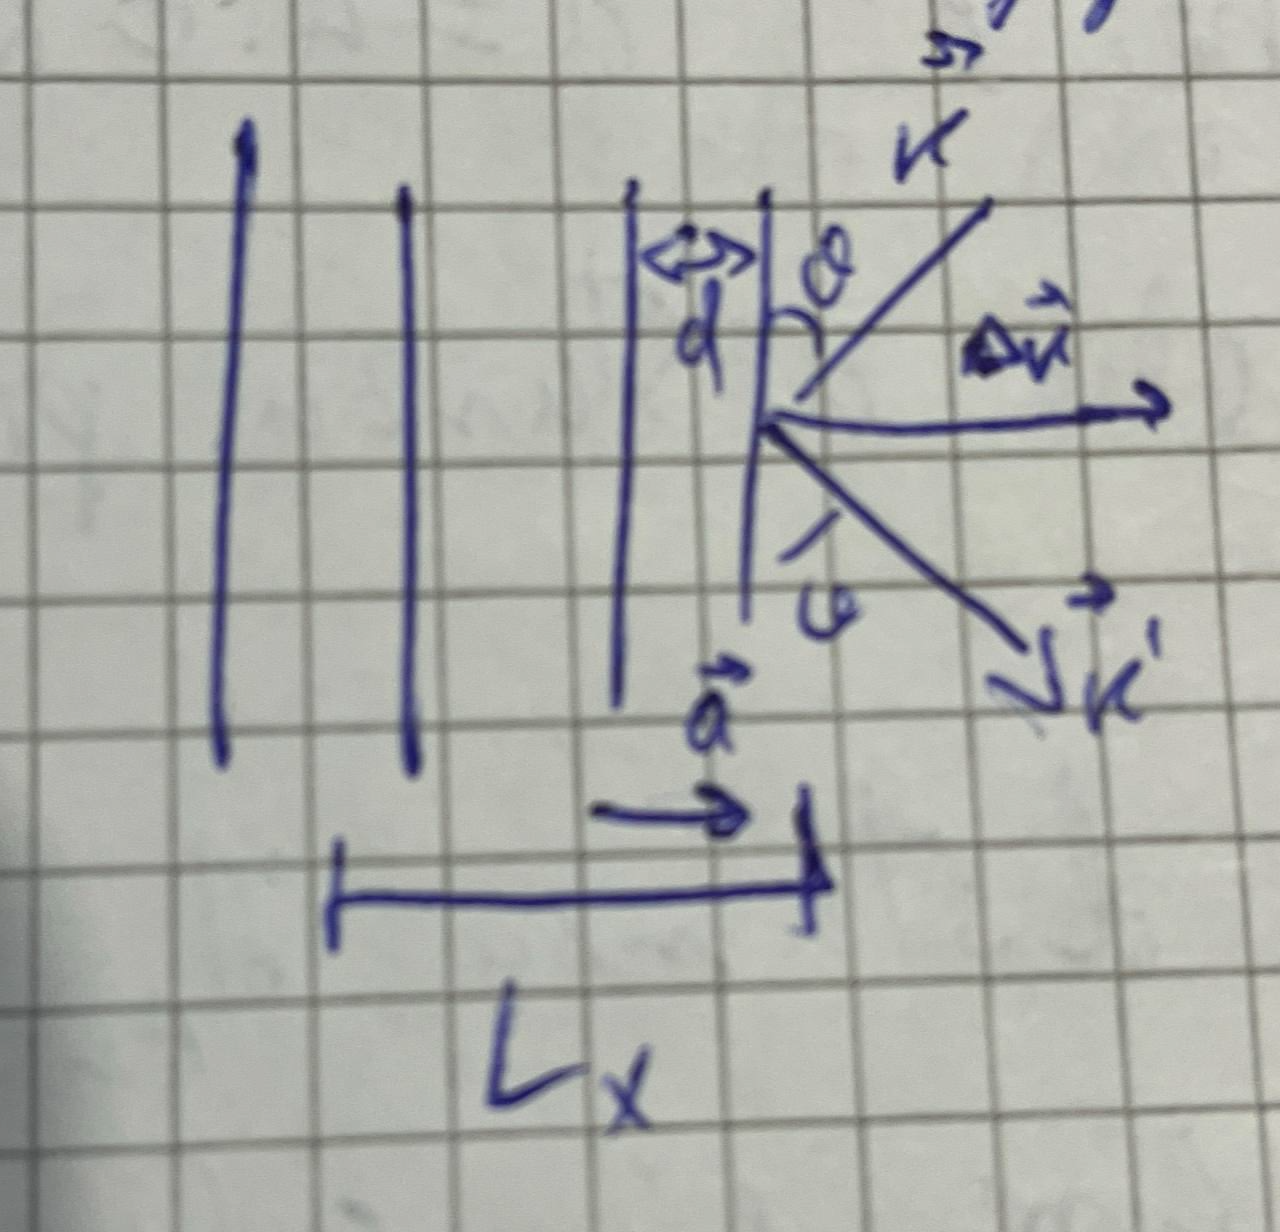
\includegraphics[width=0.5\linewidth]{img/cristalloOscillazioniLez9.png}
            \end{figure}
            \paragraph{}
                Risulta $I(x) = I_{0}(\frac{\sin ^{2} x}{x^{2}})$ con il grafico che fa così:
                \begin{figure}[h!]
                    \centering
                    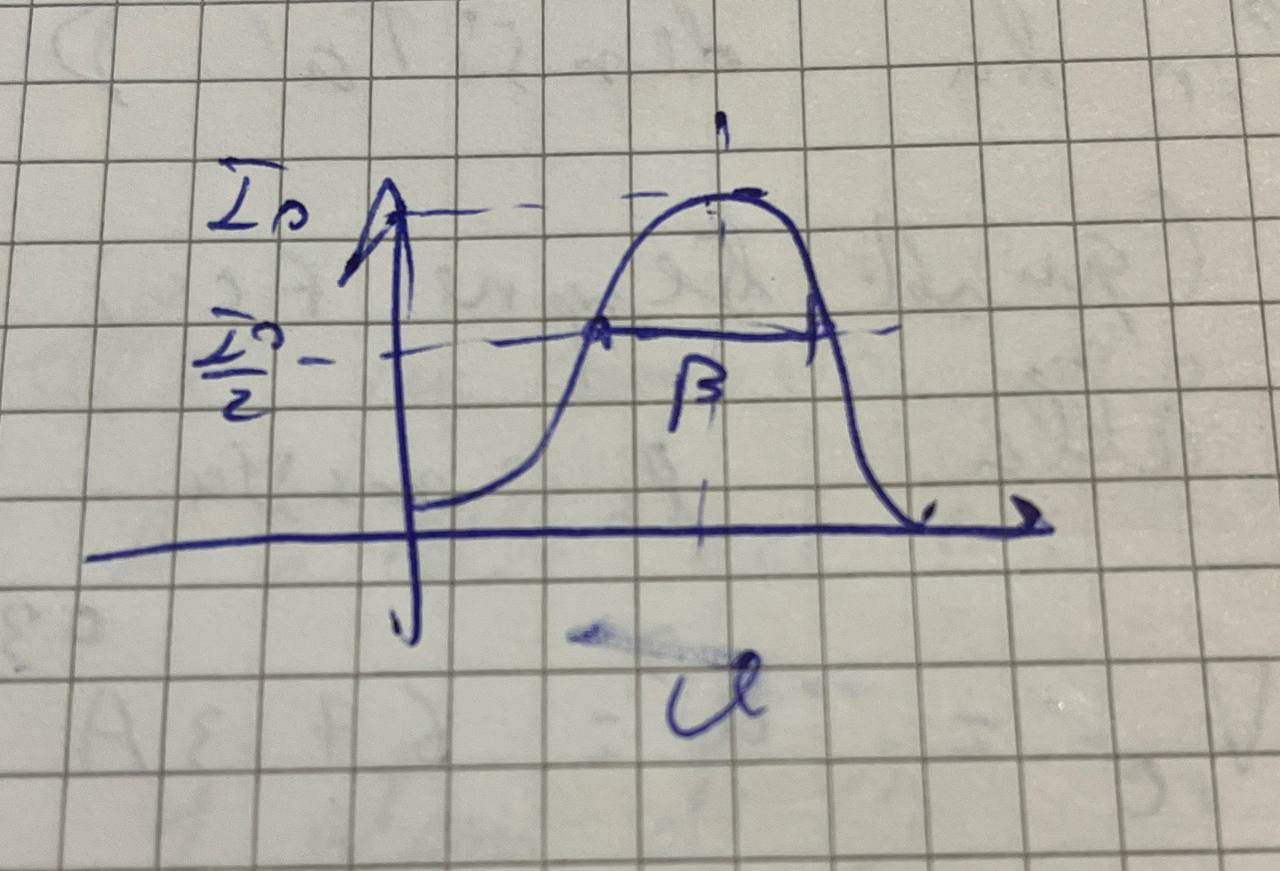
\includegraphics[width=0.5\linewidth]{img/scherrerFormulaLez9.png}
                \end{figure}
            La larghezza a metà altezza ($I(x) = \frac{I_{0}}{2}$) è pari al valore della costante elastica $\beta$ e si può ricavare tramite la \textbf{formula di Scherrer}:
            $$\beta = \frac{0.89 \lambda}{L_{x} \cos{(\vartheta)}}$$

            da cui si evince che l'unico caso nel quale i picchi sono nulli corrisponde a quello di un cristallo infinito. 
    \section{La sfera di Ewald}
            Il metodo della sfera di Ewald viene utilizzato per determinare le condizioni di 
            diffrazione all'interno del reticolo reciproco. Si parte con il mettersi nello spazio dei $\vec{k}$, che è 
            uno spazio tridimensionale dal momento che $k$ è a tre dimensioni. A questo punto si trasla $\vec{k}$ nell'origine 
            e si traccia la sfera che ha come centro $\vec{k}$ e come raggio il suo modulo: sulla circonferenza verrà identificato 
            un punto tramite l'intersezione con $\vec{k}$, il quale identificherà a sua volta il vettore del reticolo 
            reciproco $\vec{G}$ che soddisfa la condizione $\Delta \vec{k}=\vec{G}$. A questo punto si ricava $\vec{k}'$ conoscendo
            sia $\vec{k}$ che $\vec{G}$.
            \begin{figure}[h!]
                \center  
                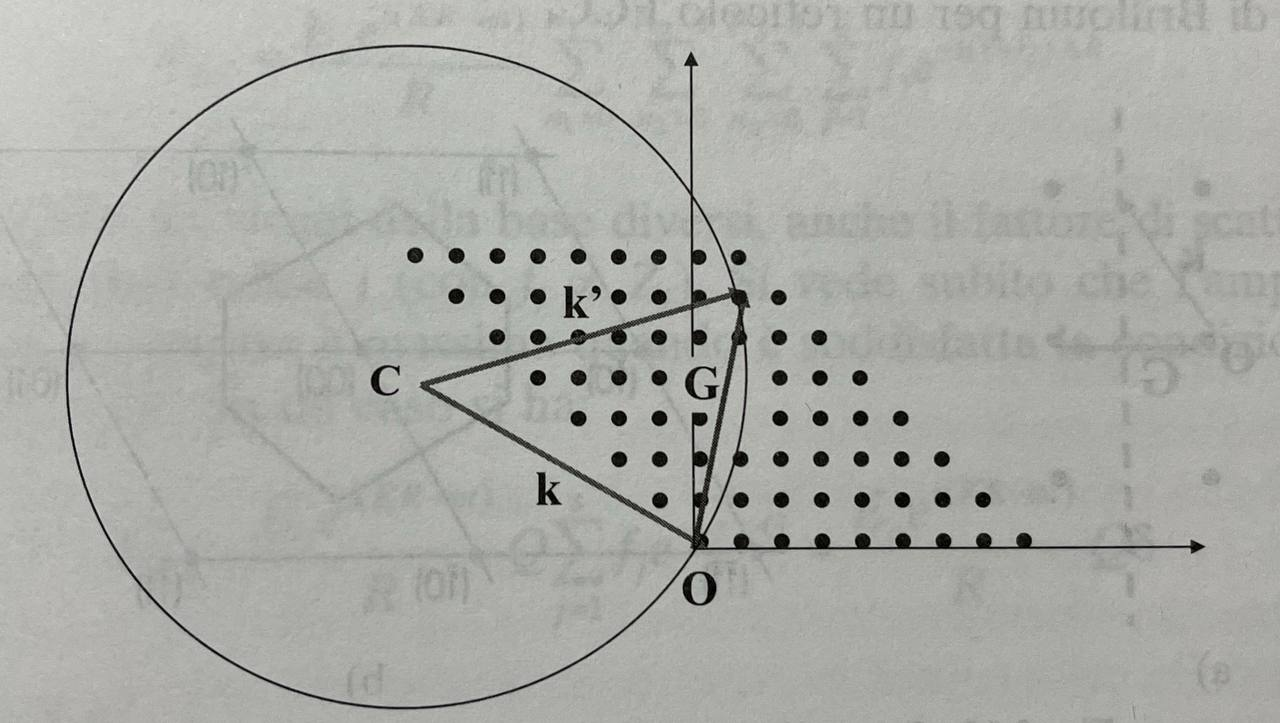
\includegraphics[width=0.6\linewidth]{img/SferaEwald.jpg}
            \end{figure}
\chapter{Modello di Sommerfeld per i metalli}
    \section{Introduzione}
        \paragraph{}
            Nel suo modello Sommerfeld assunse che gli elettroni nei solidi si comportassero come un gas perfetto, dunque si adatta ottimamente ai metalli che hanno alta concentrazione di elettroni liberi.
        \paragraph{}
            Il ruolo del reticolo in tale modello è solo quello di confinare gli elettroni in un certo volume. Partiamo con lo studio del caso monodimensionale di un solido di lunghezza $L$ lungo la direzione $x$.
            \begin{figure}[h!]
                \centering
                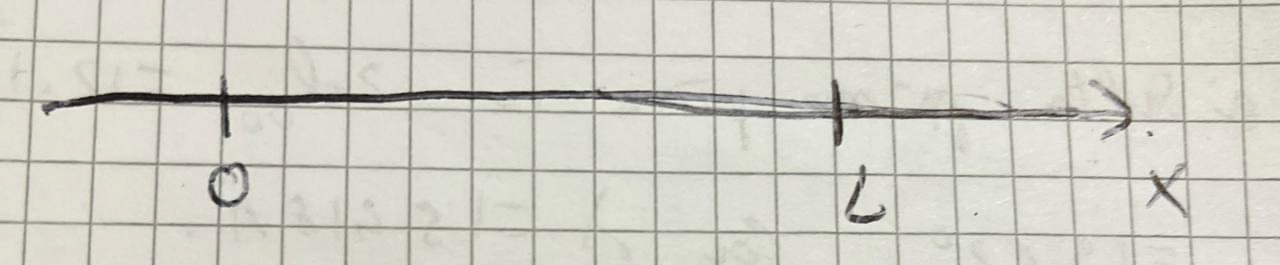
\includegraphics[width=0.5\linewidth]{img/direzioneLungoExLez12.png}
            \end{figure}
            Gli elettroni sono liberi di muoversi all'interno del solido per $x \in [0,L]$, che nel caso tridimensionale si generalizza banalmente in $(x,y,z) \in (0,0,0),(L_{x}, L_{y}, L_{z})$. Ricaviamo l'espressione dell'hamiltoniana  per questo sistema, risolvendone la relativa equazione di Schroedinger stazionaria.
        \paragraph{}
            Se gli elettroni sono liberi non c'è energia potenziale che li influenzi e dunque:
            $$\hat{H} = \frac{p^{2}}{2m_{e}}$$

            ma per giustificare il fatto che gli elettroni non balzino fuori dal solido bisogna assumere che:
            $$U(x) =\begin{cases}
                0 \quad x \in [0, L] \\
                \infty \quad \textrm{elsewhere}
            \end{cases}$$
            cioè la grande assunzione che Sommerfeld fa è che il sistema si comporti come una buca di potenziale infinita, grazie alla quale si può scrivere $\hat{H} = \frac{p^{2}}{2m_{e}}+ U(x)$ potendo comunque trascurare la funzione potenziale all'interno del solido.
            \paragraph{} Ricordando che:
            $$\frac{p^{2}}{2m_{e}} \iff - \frac{\partial ^{2}}{\partial x^{2}} \frac{\hbar}{2m_{e}}$$
            ed assumendo ragionevolmente che in $x=0$ ed $x=L$ non ci siano elettroni:
            $$\begin{cases}
                \displaystyle -\frac{\hbar}{2m_{e}}\frac{\partial ^{2} \Psi(x)}{\partial x^{2}} = E\Psi(x)  \quad x \in [0,L]\\
                \Psi(0) = \Psi(L) = 0 \quad \textrm{elsewhere}
            \end{cases}$$

            \paragraph{}
                Riscrivendo:
                $$\frac{\partial ^{2}\Psi(x)}{\partial x^{2}} = - \frac{2m_{e}E}{\hbar ^{2}} \Psi(x)$$

                ci sono due candidati a soluzione: un esponenziale oppure un seno/coseno. La prima è inadatta, perché non soddisfa le condizioni al contorno (banalmente per $x=0$ vale uno e non zero). Dunque la soluzione è del secondo tipo. \newline
               
                Posto:
                $$k = \sqrt{\frac{2m_{e}E}{\hbar ^{2}}}$$
                scrivendo la soluzione come combinazione lineare di seno e coseno:
                $$\Psi(x) = A \sin(kx) + B\cos(kx)$$
                Poiché deve annullarsi in $x=0$ ed $L=0$ risulta:
                $$\begin{cases}
                    B\cos{0} = 0 \implies B = 0 \\
                    A\sin(kL) = L \implies k_{n} = \displaystyle \frac{n\pi}{L} 
                \end{cases}$$

                da cui si ottiene:
                $$\Psi_{n}(x) = A_{n} \sin(\frac{n \pi}{L} x)$$

                Sostituendo nell'equazione di Schroedinger:
                $$-\frac{h^{2}}{2m_{e}}(-A_{n}(\frac{n\pi}{L})^{2})\sin(\frac{n \pi}{L}x) = EA_{n}\sin(\frac{n \pi}{L} x)$$
                Il fattore di normalizzazione $A_{n} = (\frac{\pi}{L})^{1/2}$ facendo i conti, cioè integrando il modulo quadro di $\Psi_{n}(x)$ e imponendo che la probabilità sia pari ad uno.

            \paragraph{}
                In definitiva:
                $$\Psi(x) = (\frac{\pi}{L})^{1/2} \sin(n \frac{\pi}{L} x)$$
                con autovalori:
                $$E_{n} = \frac{h^{2}}{2m_{e}}( n\frac{\pi}{L})^{2}$$

            \newpage
            \paragraph{}
                Graficando la $\Psi(x)$ ci si accorge che all'aumentare di $n$ aumenta il numero di semiperiodi della sinusoide nell'intervallo $x \in [0, L]$:
                \begin{figure}[h!]
                    \centering
                    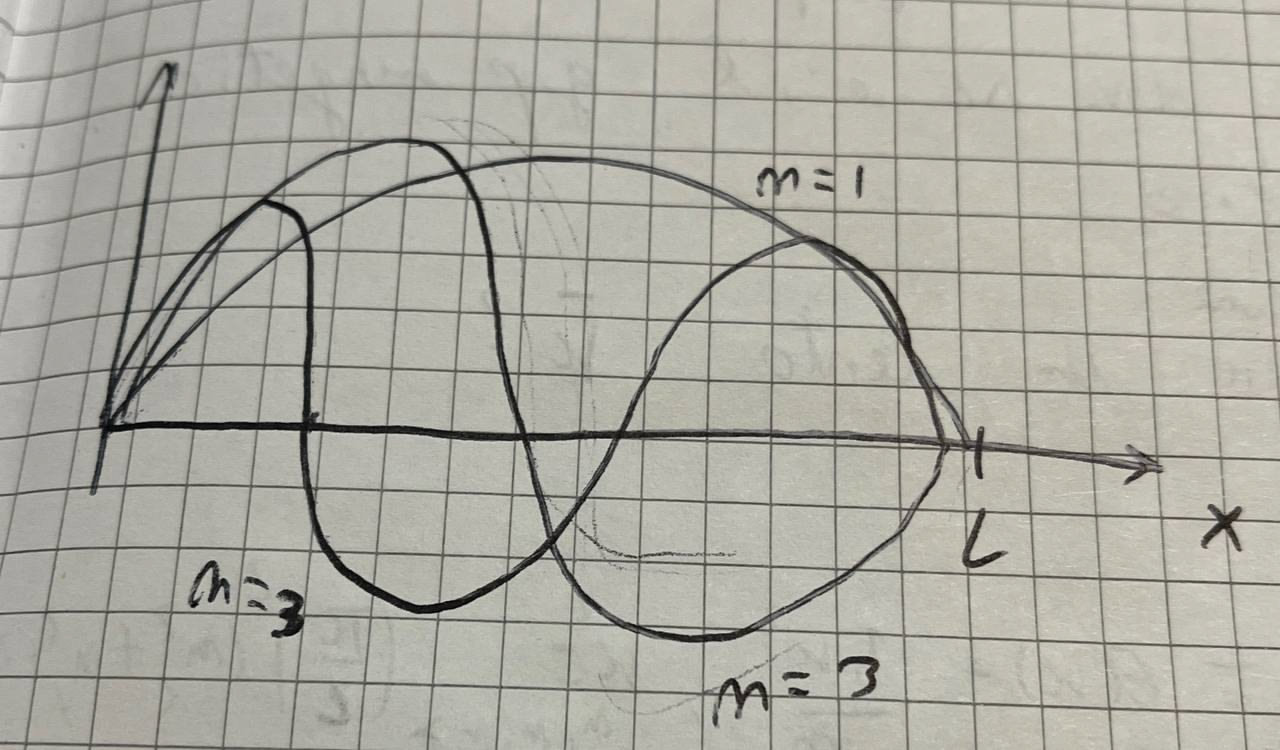
\includegraphics[width=0.5\linewidth]{img/intervalliSinLez12.png}           
                \end{figure}
                \newline
                Per quanto riguarda invece le energie, lo stato $n$ e $-n$ hanno lo stesso autovalore perché compare il quadrato. \newline
                Di nuovo, nel caso tridimensionale si generalizza con:
                $$\Psi_{n_{x}, n_{y}, n_{z}} (x,y,z) = A\sin(n_{x} \frac{\pi}{L_{x}} x)\sin(n_{y} \frac{\pi}{L_{y}} y)\sin(n_{z} \frac{\pi}{L_{z}} z)$$
                con $A= (\frac{\pi}{L})^{3/2}$
                e relativi autovalori:
                $$E_{n_{x},n_{y},n_{z}} = \frac{\hbar ^{2} \pi ^{2}}{2m_{e}} (\frac{n_{x} ^{2}}{L_{x} ^{2}}+\frac{n_{y} ^{2}}{L_{y} ^{2}}+\frac{n_{z} ^{2}}{L_{z} ^{2}})$$

                L'energia minima si ha per $(n_{x}, n_{y}, n_{z}) = (1,1,1,)$, in quanto se uno di questi tre indici è nullo la funzione d'onda è nulla ovunque e non ha senso fisico. Guardando all'espressione degli autovalori è facile desumere che gli stati per i quali la somma degli indici è uguale hanno energia uguale, per esempio $(1,1,,2)$ e $(2,1,1)$.

        \section{Sfera di Fermi e DOS}
            \paragraph{}
                Ci si chiede: quanti stati ci sono per $k \leq \bar{k}$, con $\bar{k}$ un certo valore fissato di $k$? Facendo un disegno in 2D si ottiene una circonferenza all'interno del quale ci sono gli stati che soddisfano tale relazione, mentre in 3D si avrà una sfera. Ricordiamo che lo spazio che stiamo considerando è discretizzato, cioè i punti sono terne di numeri interi $k_{x}, k_{y}, k_{z}$ (in figura rappresentato solo in due dimensioni).
               \newpage
                \begin{figure}[h!]
                    \centering
                    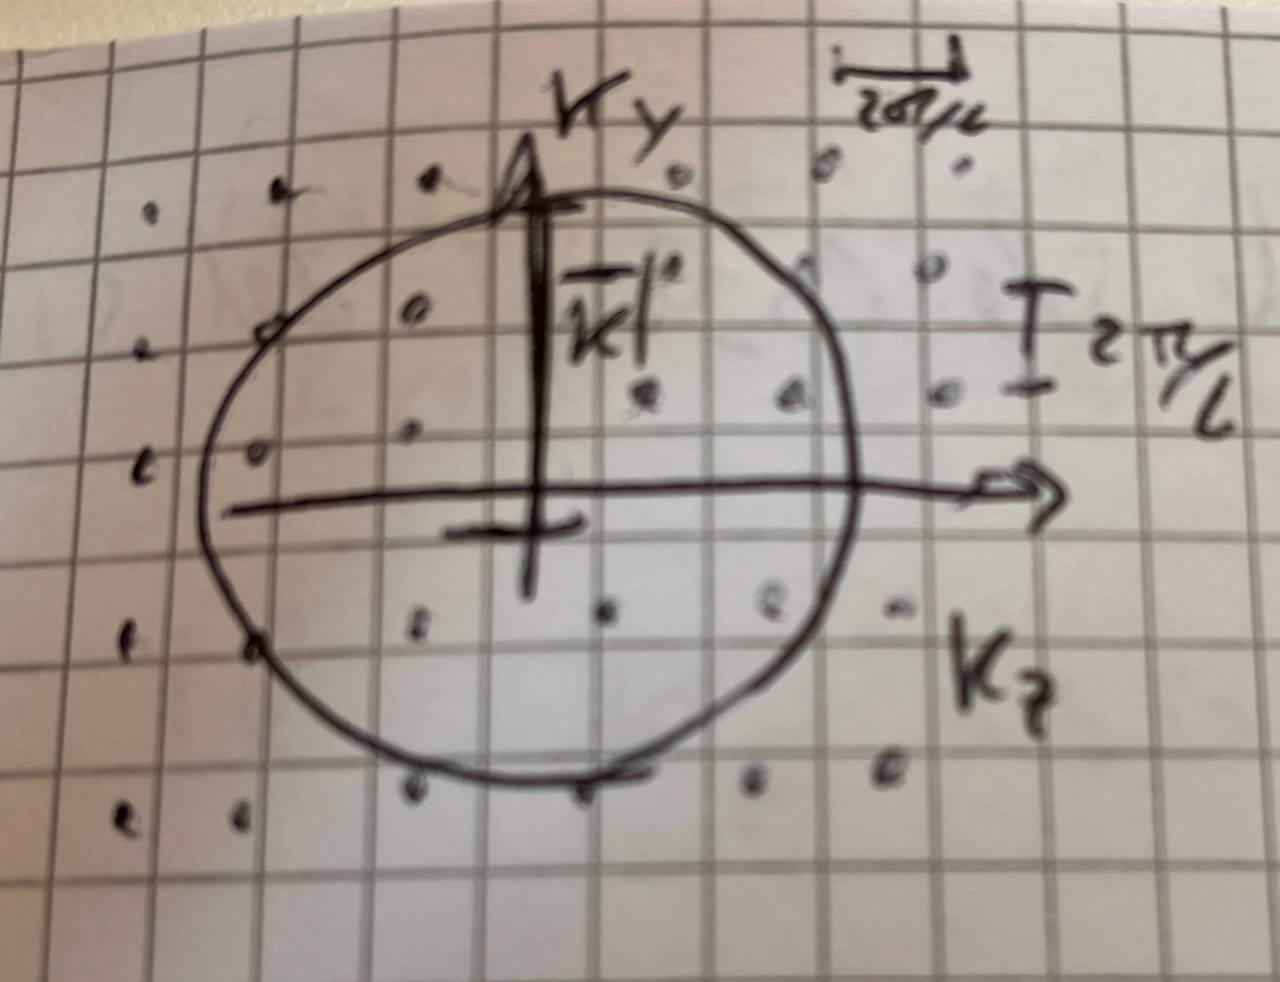
\includegraphics[width=0.5\linewidth]{img/spazioDiFermiLez12.png}
                \end{figure}
                \paragraph{}
                In tre dimensioni è possibile associare ad ogni stato un volumetto $\displaystyle \Delta k = (\frac{\pi}{L})^{3}$ e quindi, alla buona, si può affermare che il numero di stati sia dato dal rapporto fra il volume della sfera e quello del volumetto.

                \paragraph{}
                    Sia allora $G'(\bar{k})$ il numero di stati per $k \leq \bar{k}$. La sfera ha volume $\displaystyle 4 \frac{\pi}{3}\bar{k}^{3}$ e dunque:
                    $$G'(\bar{k}) = \frac{4}{3}\pi\bar{k}^{3} \cdot \frac{1}{(\frac{\pi}{L})^{3}}$$

                    Ogni stato va considerato due volte per via dello spin, dunque si moltiplica per due. Tuttavia un solo ottante dello spazio 3D è indipendente, perché abbiamo ricavato prima che quelli dalla somma uguale sono uguali e dunque va diviso per otto, ottenendo in definitiva un fattore moltiplicativo $1/4$. Sviluppando l'espressione:
                    $$G'(k) = \frac{\bar{k}^{3}}{3 \pi^{3}}L^{3}$$
            \paragraph{}
                In modo analogo, per ricavare il numero di stati ad energie minori (aka livelli energetici) di $\bar{E}$, basta ricordare la relazione:
                $$\bar{E} = \frac{\hbar ^{2}}{2m_{e}}\bar{k}^{2} \implies \bar{k} =\sqrt{ \frac{2m_{e}\bar{E}}{\hbar ^{2}}}$$

                e sostituire nella relazione precedente, ricavando:
                $$G'(\bar{E}) = \frac{L^{3}}{2 \pi ^{2}} (\frac{2m_{e}\bar{E}}{\hbar ^{2}}) ^{3/2}$$

            \paragraph{}
                Calcolare il numero di stati totale però è da sfigati e dunque definiamo la stessa grandezza \textbf{per unità di volume}, tenendo conto che $V=L^{3}$:
                $$G(E) = \frac{G'(E)}{V} = \frac{(2m_{e}) ^{3/2}}{3 \pi^{2}\hbar^{3}} E^{3/2}$$

                Stesso discorso va fatto per $G(k)$. Scrivendo in modo più compatto tutte quelle costanti sotto un unico termine:
                $$\gamma = \frac{(2m_{e})^{3/2}}{2 \pi^{2} \hbar ^{3}} = 1.06 \cdot 10^{56} m^{-3} \cdot J^{-3/2}$$
                risulta:
                $$G(E) = \frac{2}{3} \gamma E^{3/2}$$

            \paragraph{}
                Le cose che stiamo per trattare valgono in via generale e non solo per il modello di Sommerfeld. Definiamo \textbf{l'energia di Fermi} a temperatura nulla, cioè il livello di energia per il quale:
                $$\begin{cases}
                    E \leq E_{F} \quad \quad \textrm{Stati occupati} \\
                    E> E_{F} \quad \quad \textrm{Stati vuoti}
                \end{cases}$$
                

            Sia $n$ il numero di eletttoni per unità di volume. Per $T=0K$ risulta:
            $$n = G(E_{F}) = \frac{2}{3} \gamma E_{F} ^{3/2} \implies E_{F} = (\frac{3}{2\gamma}n)^{2/3}$$
            Per un metallo $n \simeq 10^{28} \div 10^{29} m^{-3}$ e dunque:
            $$E_{F} \simeq (\frac{10^{29}}{10^{56}})^{2/3} \simeq 10^{-18}J \simeq 1 \div 10 eV$$
            che per la scala elettronica sono energie enormi.
            \begin{figure}[h!]
                \centering
                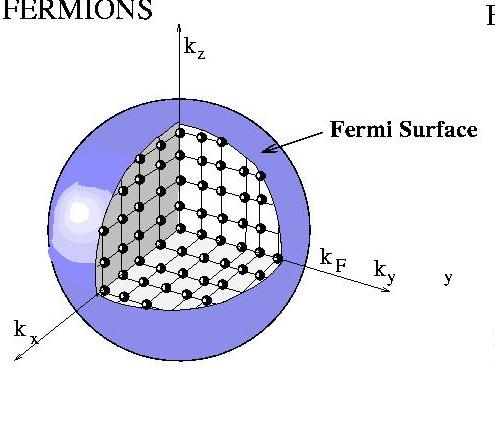
\includegraphics[width=0.5\linewidth]{img/FermiSurfaceLez12.png}
                \caption{Superficie di Fermi nello spazio dei $k$}
            \end{figure}

            \paragraph{}
                Nello spazio degli stati, la sfera di raggio $\bar{k}$ identificata da $G(k)$ è detta \textbf{superficie di fermi}. A temperatura ambiente $k_{b}T \simeq 25meV$, dunque gli elettroni agli stati inferiori, che necessitano di energie prossime a quelle di Fermi per fare il salto di livello energetico, rimarranno dove stanno. Quelli che possono muoversi più liberamente sono agli stati più in alto con livelli di energia alti.

            \paragraph{}
                Il $k_{F}$ associato ad $E_{F}$ è chiamato, con abuso perché dimensionalmente non omogeneo ad un momento, \textbf{momento di Fermi} e vale:
                $$k_{F} = \frac{\sqrt{2m_{e}E_{F}}}{\hbar} \simeq 1 \textrm{\si{\angstrom}} ^{-1}$$
                Allo stesso modo si può definire la \textbf{temperatura di Fermi}:
                $$T_{F} = k_{b}E_{F} \simeq 10^{4} \div 10^{5}  K$$
                che è stupidamente alta e dunque di solito si utilizza come riferimento il rapporto:
                $$\frac{k_{b}T}{E_{F}} = \frac{T}{T_{F}}$$
                Infine si può definire la velocità di Fermi:
                $$v_{F} = \sqrt{\frac{2E_{F}}{m_{e}}} \simeq 10^{5} \div 10^{6} m/s$$
                Possiamo esprimere il numero di livelli energetici minori di $E$ per unità di volume $G(E)$ come l'integrale di una certa funzione $N(E)$, che chiameremo \textbf{densità di stati} (Density of States, DOS):
                $$G(E)  = \int_{0} ^{E} N(E')dE'$$
                La quantità $N(E)dE$ è il numero di stati per unità di volume nella porzione di energie di centro $E$ e raggio $dE$.\newline
                Si può scrivere allora:
                $$N(E) = \frac{\partial G(E)}{\partial E}$$
                che nel modello di Sommerfeld equivale a dire:
                $$N(E) = \frac{\partial}{\partial E} (\frac{2}{3}\gamma E^{3/2}) = \gamma E^{1/2}$$
            \newpage
    \section{Effetto della temperatura}
        \paragraph{}
            Le considerazioni che abbiamo fatto finora valgono per lo zero termico, dunque bisogna capire in che modo la temperatura influenza l'espressione della DOS. Introduciamo, a tal proposito, la funzione di Fermi-Dirac:
            $$f(E, T) = \frac{1}{1+\exp{(\frac{E-E_{F}(T)}{k_{b}T})}}$$

            Tale funzione rappresenta la \textbf{probabilità} che alla temperatura $T$ lo stato al livello di energia $E$ risulti occupato.
            
            Per $E=E_{F}$ risulta $f(E,T) = \frac{1}{2}$, dunque l'energia di Fermi è il livello di energia tale per cui c'è il 50\% di probabilità di trovare lo stato occupato.
            \begin{figure}[h!]
                \centering
                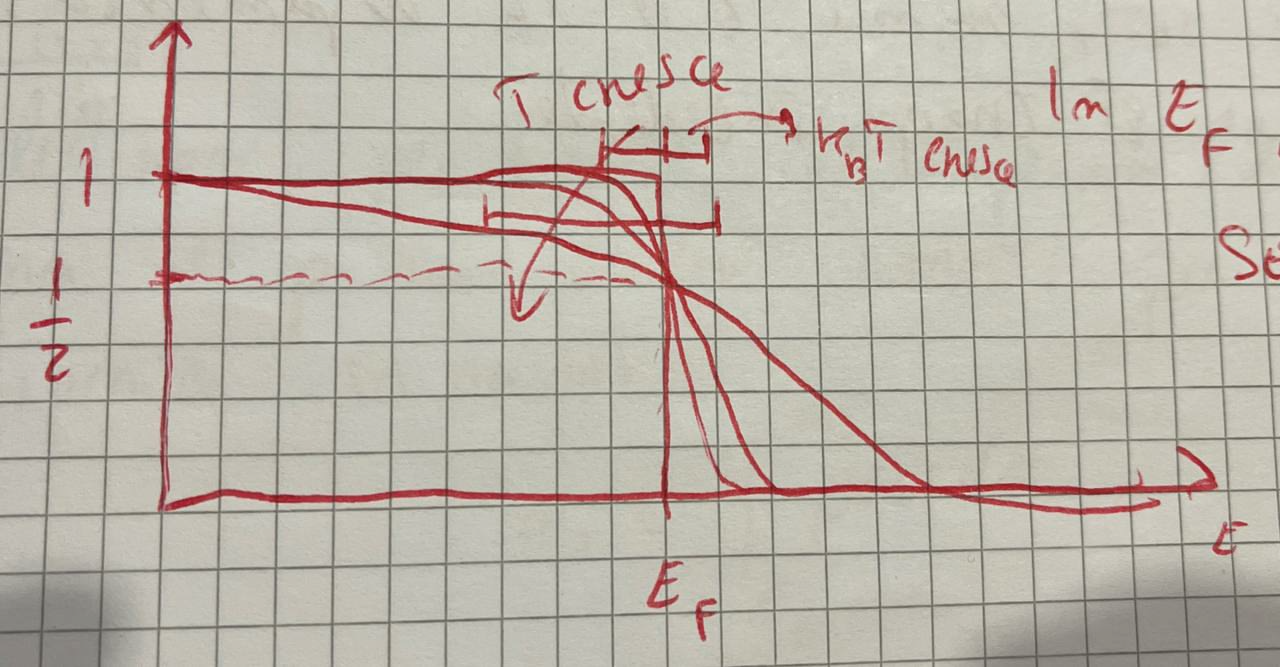
\includegraphics[width=0.5\linewidth]{img/RobettaFermiLez12.png}
                \caption{Funzione di Fermi-Dirac variando la temperatura}
            \end{figure}

            A temperatura nulla vale:
            $$n = \int_{0} ^{E_{F}} N(E)dE$$

            Per $T>0K$ alcuni stati sotto $E_{F}$ sono vuoti ed alcuni pieni sopra. Introduciamo allora:
            $$\rho_{T}(E) = N(E)f_{T}(E)$$
            avendo fissato $T$. Dimensionalmente si trova di un peso ad ogni item dello spazio degli stati.
            $$n_{T>0K} = \int_{0} ^{\infty} \rho_{T} (E) dE = \int_{0} ^{\infty} \frac{N(E)}{1+\exp{(\frac{E-E_{F}}{k_{b}T})}}$$

            dove integriamo fino all'infinito perché a rigore $f(E,T)$ non si annulla mai.

        \paragraph{}
            L'energia di Fermi dipende dalla temperatura, ma più propriamente $E_{F}(T)$ si chiama \textbf{potenziale chimico}, indicato di solito con $\mu (T)$. Noi però continuiamo a chiamarlo $E_{F}(T)$.

            Se sviluppiamo in serie (?):
            $$E_{F}(T) = E_{F}(0)[1 - \frac{\pi ^{2}}{12}(\frac{k_{b}T}{E_{F}(0)})^{2}+ \cdots ]$$
            gli altri termini li trascuriamo e teniamo conto solo del primo termine correttivo: c'è una dipendenza da $T$ ma non è troppo incidente.


      \section{Effetto Termoionico}
        \paragraph{}
            Riscaldando un metallo questo emette elettroni. Gli elettroni ad energia più alta non saltano fuori dal metallo in quanto l'energia di barriera è sempre maggiore di $E_{F}(T)$.
            \begin{figure}[h!]
                \centering
                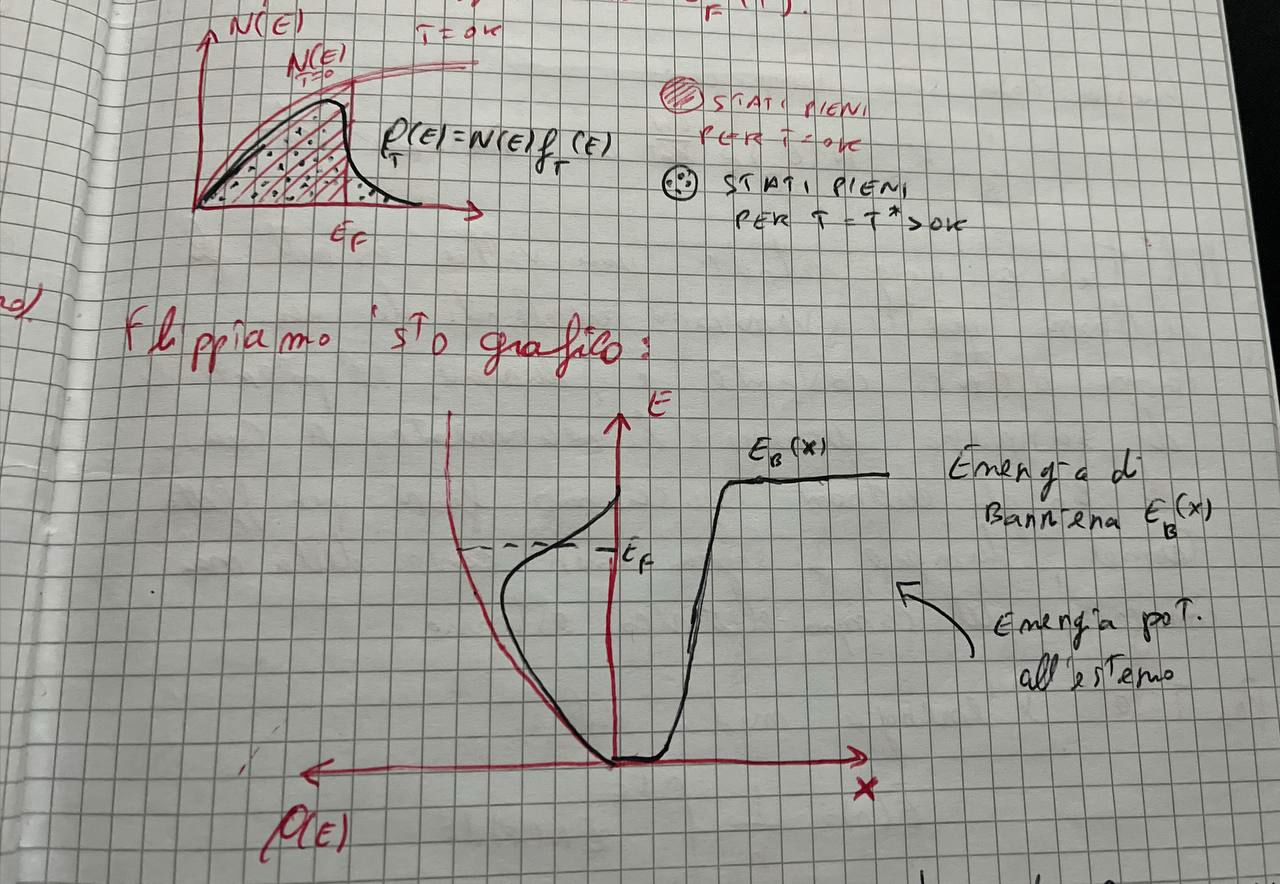
\includegraphics[width=0.85\linewidth]{img/EffettoTermoionicoBarrieraLez12.png}
            \end{figure}
            La differenza $E_{B}(x)-E_{F}(x)$ è chiamata \textbf{potenziale di lavoro} (o di estrazione) $E_{W} = E_{B} - E_{F}$.
            Gli elettroni, per $T>0K$, che superano l'energia di barriera e possono allora essere emessi per effetto termoionico saranno in numero:
            $$n_{T}  =\int_{E_{B}} ^{\infty} \rho(E)dE$$

            da cui:
            $$n_{T} = \int_{E_{B}} ^{\infty} \frac{N(E)}{1 + \exp{(\frac{E-E_{F}}{K_{B}T})}}dE \simeq K_{B}TN(E_{B})\exp{(-\frac{E_{W}}{K_{B}T})}$$

            avendo approssimato $N(E) \simeq N(E_{B}$, $1 + \exp{(\frac{E-E_{F}}{K_{B}T})} \simeq \exp{(\frac{E-E_{F}}{K_{B}T})}$ ed ipotizzando che l'emissione di elettroni sia isotropa. Questa cosa sarà proporzionale a:
            $$K_{B}TN(E_{B})\exp{(-\frac{E_{W}}{K_{B}T})} \propto TN(E_{F})\exp{(-\frac{E_{W}}{K_{B}T})}$$

            \paragraph{Che cazzo ho scritto non mi ricordo manco io}
                Nel tubo a raggi catodici, una volta estratti gli elettroni questi venivano accelerati da un campo elettrico costante. Allora il potenziale di barriera decresceva linearmente. A causa di ciò gli elettroni sgusciano fuori per effetto tunnel e dunque bisogna tener conto della \textbf{innocenza del campo elettrico esterno}.

            \paragraph{}
                Per $T = 0K$ l'energia media vale:
                $$E(0) = \frac{1}{n} \int_{0} ^{E_{F}} EN(E)dE$$
                dove $n$ è il numero di elettroni per unità di volume ed $N(E)dE$ il numero di stati per unità di volume ad energie vicine ad $E$ di $dE$.
                Quest'integrale non è altro che la somma pesata degli stati con pesi la loro energia, dunque una media pesata a coefficiente $N(E)dE$ delle energie $dE$.\\
                Dunque nel modello di Sommerfeld:
                $$\bar{E}(0) = \frac{1}{n} \int_{0} ^{E_{F}} \gamma E^{3/2} d E = \frac{2}{5} \frac{\gamma}{n}E^{5/2}$$
        
                poiché $n= \displaystyle \frac{2}{3} \gamma E_{F} ^{3/2} \implies \bar{E}(0) = \frac{3}{5} E_{F}$, dove $\bar{E}(0)$ è l'energia media per $T=0K$.

        \section{Il calore specifico e la capacità termica}
            \paragraph{}
                La capacità termica, ricordiamo, è la derivata del calore rispetto alla temperatura:
                $$C_{Termica} = \frac{\delta Q}{\partial T}$$
                mentre il calore specifico è il rapporto fra la capacità termica e la massa $m$ dell'oggetto considerato. Il $\delta Q$ sottolinea il fatto che il calore \textbf{non} è una differeziale esatto. 
                Definiamo la capacità termica elettronica come:
                $$C_{el} = \frac{\delta Q}{\partial T} \cdot\frac{1}{V}$$
                Se non c'è lavoro di volume, $\delta Q = dU$, che è la variazione di energia termodinamica totale. Risulta allora:
                $$C_{el} = \frac{1}{V} \cdot \frac{dU}{dT}$$
                L'energia media, che abbiamo visto prima, si può scrivere con buona approssimazione come:
                $$\bar{E}(T) = \frac{1}{n} \frac{U}{V} \implies \frac{U}{V} = n\bar{E}(T)$$
                dunque:
                $$C_{el} = n \frac{d\bar{E}(T)}{dT}$$
                Ora che la temperatura non è nulla, bisogna tener conto degli stati occupti anche altre $E_{F}$, cioè portare $\rho(E) = N(E)f(E,T)$ nell'integrale:
                $$\bar{E}(T) = \frac{1}{n} \int_{0} ^{\infty} E \rho(E)dE = \frac{1}{n} \int_{0} ^{\infty} E\frac{N(E)}{1+\exp{(\frac{E-E_{F}}{k_{B}T})}}dE$$
                Con tutte le approssimazioni del caso otteniamo un'espressione lineare in $T$:
                $$C_{el}(T) = \frac{\pi ^{2}}{3} N(E_{F}) k_{B} ^{2} T = \gamma_{S} T$$
                dove $\gamma_{S}$ è detta \textit{costante di Sommerfeld}.
                Classicamente si utilizza la statistica di Boltzmann al posto di quella di Fermi-Dirac e risulta, sempre classicamente:
                $$C_{el}(T) = n \frac{\partial}{\partial T} \bar{E}(T) = n \frac{\partial}{\partial T} (\frac{3}{2}k_{B}T) = \frac{3}{2}nk_{B}$$
                che è una quantità costante rispetto alla temperatura.
                Esplicando invece $N(E_{F})$ per la $C_{el}(T)$ "quantistica", moltiplicando e dividendo per $2E_{F}$:
                $$C_{el} = \frac{\pi ^{2}}{3} \gamma E_{F} ^{1/2}2E_{F} \frac{k_{B} ^{2}T}{2E_{F}} = \frac{\pi ^{2}}{2}k_{B} n(\frac{k_{B}T}{E_{F}})$$
                avendo scritto $nk_{B} =\displaystyle \frac{\pi^{2}}{3} \gamma E^{1/2} E_{F}$.
                Il termine $\frac{k_{B}T}{E_{F}}$ è stupidamente piccolo, motivo per il quale a livello quantistico la capacità elettronica è piccola. A differenza, infatti, della statica di Boltzmann, che tratta gli elettroni tutti in modo uguale, il principio di Pauli preclude il fornire energia agli stati più interni alla sfera di Fermi nello spazio dei momenti, perché sopra di loro non ci sono stati vuori da occupare e dunque gli unici che fanno il salto sono vicino o poco fuori la sfera.

\chapter{Modello di Drude per la conduzione nei metalli}
    \section{Introduzione e considerazioni per campi elettrici costanti}
        \paragraph{}
        Quello di Drude è un modello semiclassico. Consideriamo il solito spazio dei momenti $\vec{k}$. In assenza di stimoli esterni e per temperature nulle, tutti gli stati nella sfera di Fermi sono occupati. Ricordimo le relazioni fra energia e momento di Fermi per $T=0K$:
        $$E_{F} = \frac{\hbar ^{2}k^{2} _{F}}{2m_{e}} \implies k_{F} = \sqrt{\frac{2m_{e}E_{F}}{\hbar ^{2}}}$$
        Cosa succede se applichiamo un campo elettrico?
        A temperatura nulla, tra gli stati pieni $\forall k$ c'è, nella sfera di Fermi (SF), anche il volume associato a $-k$ e dunque:
        $$\sum_{i} ^{n_{stati} \in \textrm{SF}} \vec{k}_{i0} = 0$$
        dove $k_{i0}$ è il momento $i-$esimo per $T=0K$.
        Questo può essere visto in termini di velocità:
         $$\sum_{i} ^{n_{stati} \in \textrm{SF}} \vec{v}_{i0} = 0$$
         e dunque anche la velocità media sarà nulla:
         $$ \vec{v}_{m0} = \sum_{i} ^{n_{stati} \in \textrm{SF}} \vec{v}_{i0} = 0$$
         Esaminiamo  il caso nel quale $\vec{E} = \textrm{costante}$. La forza esercitata su un generico elettrone nel metallo è:
         $$\vec{F}_{e} = -e\vec{E} = m_{e} \frac{d\vec{v}}{dt}$$
         con $\displaystyle \frac{d \vec{v}}{dt}$ l'accelerazione dell'elettrone. Equazione differenziale risolta:
         $$\vec{v}_{i} (t) = \vec{v}_{i0} - \frac{e \vec{E}}{m_{e}} t$$
         con $\vec{v}_{i0}$ velocità dell'elettrone per $t=0$.
         Segue, facendo la media all'istante $t$:
         $$\vec{v}_{m} = \frac{1}{N} \sum_{i} ^{N} \vec{v}_{i} (t) = \frac{1}{N} \sum_{i} ^{N}\vec{v}_{i0} - \frac{1}{N} \sum_{i} ^{N} \frac{e}{m_{e}}\vec{E}t = - \frac{e \vec{E}}{m_{e}} \tau$$

         Chiariamo i passaggi: la somma delle velocità iniziali statisticamente si annulla per ogni tempeatura, perché gli stati saranno ugualmente dentro e fuori la sfera. Il secondo termine è una costante, omogenea ad una accelerazione, moltiplicata per un tempo medio $\tau = \frac{t}{N}$. Nota: onestamente non so che senso abbia quest'ultimo passaggio, non vedo perché fissando l'istante si possa definire il tempo medio, che andrebbe valutato perlomeno su un intervello infinitesimo di $t$, ma vabbè. 
         \paragraph{}
            Ci si dovrebbe aspettare che la velocità media cresca indisturbata man mano che passa il tempo, ma ovviamente non è così. Nel modello di Drude il meccanismo che impedisce agli elettroni di accelerare in modo definito è trattato alla stregua di una forza viscosa. Allora tutto ciò che è scritto sopra \textbf{è sbagliato}: si introduce un termine correttivo $\displaystyle k\frac{\vec{v}_{m}}{m_{e}}$ nell'espressione dell'accelerazione, con $k$ che ha le dimensioni di un attrito viscoso:
            $$\frac{d\vec{v}_{m}}{dt} = - \frac{e\vec{E}}{m_{e}} - k \frac{\vec{v_{m}}}{m_{e}} = -\frac{e\vec{E}}{m_{e}}-\frac{1}{\tau}\vec{v}_{m}$$
            dove $\displaystyle \tau = \frac{m_{e}}{k}$. Dunque dopo un certo tempo si raggiunge una $\vec{v}_{m}$ a regime dove, con l'annullarsi del termine tempovariante, risulta:
            $$\frac{d}{dt}\vec{v}_{m} + \frac{1}{\tau} \vec{v}_{m} = - \frac{e\vec{E}}{m_{e}} \stackrel{t \to \infty}{\implies} \vec{v}_{m} = - \tau\frac{e\vec{E}}{m_{e}} = - \mu_{e} \vec{E}$$
            dove la quantità $\displaystyle \mu_{e} = \frac{e \tau}{m_{e}}$ è la \textbf{mobilità elettronica}, misurata in $\textrm{cm}^{2}\cdot V \cdot s^{-1}$ (utilizzando come unità di misura della velocità e del campo elettrico rispettivamente $\textrm{cm} \cdot s^{-1}$ e $V \cdot cm^{-1}$).
            Riprendiamo l'equazione differenziale di prima. L'omogenea associata è:
            $$\vec{v}_{m} = \vec{v}_{m0} e^{-t/\tau}$$
            con $\vec{v}_{m0}$ velocità media per $\vec{E} =0$ e $\tau$ tempo caratteristico per il quale la velocità decade, cioè il tempo fra un interazione dell'elettrone con il reticolo ed un altra (dire che gli elettroni sbattono contro il reticolo è una cosa ritardata che il king della conduzione, Peter Debye, spiega con il suo modello fortissimo che vediamo boh penso fra due lezioni).
        \paragraph{}
            La conducibilità elettronica $\sigma$ è localmente definita dall'espressione vettoriale della legge di Ohm:
            $$\vec{J} = \sigma \vec{E} = \frac{1}{\rho} \vec{E}$$
            La densità di corrente è, per definizione:
            $$\vec{J} = ne\vec{v}_{n}$$
            dove sostituendo la $\vec{v}_{n}$ otteniamo:
            $$\vec{J} = \frac{ne^{2}\tau}{m_{e}}\vec{E}$$
            da cui per confronto:
            $$\sigma = \frac{ne^{2}\tau}{m_{e}}$$
            la quale si misura in $\Omega^{-1}\cdot \textrm{cm}^{-1}$
            Nei metalli le resistività viaggiano nell'ordine del $\mu \Omega \cdot \textrm{cm}$, dunque con conducibilità dell'ordine di $10^{6} \Omega^{-1} \textrm{cm }^{-1}$
            Con questi ordini di grandezza, poiché il resto dei termini nell'espressioni di $\sigma$ sono costanti, si ricavano valori di $\tau \simeq 10^{-14} \div 10^{-13} s$
            In termini di superficie di Fermi, vuol dire che a tutti gli elettroni sarà aggiunto un $\vec{k}_{m} = \displaystyle \frac{m}{\hbar} e \vec{v}_{m}$ al relativo $\vec{k}_{i}$.
            L'effetto complessivo nello spazio dei momenti è quello di traslare la sfera di Fermi di $\vec{k}_{m}$. Per un metallo, $n \simeq 10^{28}$ e dunque:
            $$\mu_{n} = \frac{\sigma}{n e} \simeq \frac{10^{8}}{10^{28} \cdot 10^{-19}} \simeq 10^{-1}m^{2}V^{-1}s^{-1} = 10^{2}$$
            In generale il range di valori per le conducibilità elettroniche è:
            $$\mu \simeq 10^{2} \div 10^{0} \frac{\textrm{cm}^{2}}{V \cdot s}$$
            dunque:
            $$E \simeq 1V \implies \vec{v}_{m} \simeq 10^{-1} \div 10^{-3} m/s \leq V_{F}$$
            La distanza percorsa fra un "urto" e l'altro sarà:
            $$l = v_{F} \tau \simeq 10 \div 10^{3} \textrm{\si{\angstrom}}$$
            Un'ulteriore espressione di $\sigma$ allora è:
            $$\sigma = \frac{ne^{2}l}{m_{e}v_{F}}$$
    \section{Considerazioni per campi elettrici sinusoidali}
        Vediamo ora per $\vec{E}$ che varia con legge sinusoidale:
        $$\vec{E} = \vec{E}_{0}e^{-j \omega t}$$
        l'omogenea è la stessa di prima, ovviamente. La particolare sarà del tipo:
        $$\vec{v}_{m} = \vec{v}_{m} e^{-j \omega t} \implies -j \omega \vec{v}_{m0}e^{-j \omega t} + \frac{\vec{v}_{m0}}{\tau} e^{-j \omega t} = - \frac{e \vec{E}_{0}}{m_{e}}e^{-j \omega t}$$
        da cui si ricava $\vec{v}_{m0}$. Risulta:
        $$\vec{v}_{m0}(1-j \omega \tau) = - \frac{e \vec{E}_{0} \tau}{m_{e}} \implies \vec{v}_{m0} = - \frac{e \vec{E}_{0} \tau}{m_{e}(1- j \omega \tau)}$$
        dunque la velocità degli elettroni è, con campo elettrico sinusoidale:
        $$\vec{v}_{m} = -\frac{e \vec{E} \tau}{m_{e}(1- j \omega \tau)}$$
        È importante che $\vec{E}_{0}$ sia il campo che vedono tutti gli elettroni oscillatni di pulsazione $\omega$, così da avere tutti la stessa velocità media $\vec{v}_{m}$. Per confronto, moltiplicando ambo membri per $-ne$, si ricava la conducibilità:
        $$-ne\vec{v}_{m} ) = \frac{e^{2}ne \tau}{m_{e}} \cdot \frac{\vec{E}}{1- j\omega \tau} = \frac{\sigma_{0}}{1 - j \omega \tau}\vec{E} = \sigma \vec{E}$$
        Analizziamo l'espressione della conducibilità:
        $$\sigma = \frac{\sigma_{0}}{1 - j \omega \tau}$$
        Se $\omega \tau << 1 \implies \sigma(\omega) \simeq \sigma_{0}$ e dunque la conducibilità è praticamente indipendente dalla frequenza. Nel caso opposto, per $\omega \tau >>1$ risulta:
        $$\sigma(\omega) \simeq j \frac{\sigma_{0}}{\omega \tau}$$
        e cioè gli elettroni rispetto al campo elettrico sono in opposizione di fase.
        Dall'equazione di continuità della corrente elettrica:
        $$\vec{J} = \frac{\partial \vec{P}}{\partial t}$$
        con $\vec{P}$ vettore di polarizzazione elettrica, si ricava la relazione nel dominio dei fasori:
    $$\vec{J} = - j \omega \vec{P} = - j \omega \varepsilon_{0} ( \varepsilon_{r} - 1) \vec{E}$$
    Poiché $\vec{J} = \sigma \vec{E}$, ri ricava per confronto:
    $$\sigma \vec{E} = - j \omega \varepsilon_{0}(\varepsilon_{r}-1)\vec{E} \implies \varepsilon_{r} = 1 + \frac{j \sigma}{\omega \varepsilon_{0}}$$
    In definitiva, sostituendo l'espressione di $\sigma$:
    $$\varepsilon_{r}(\omega) = 1 + \frac{j}{\varepsilon_{0} \omega} \frac{\sigma_{0}}{(1- j \omega \tau)}$$
    Il termine immaginario nell'espressione della costante dielettrica relativa $\varepsilon_{r}$ tiene conto dell'assorbimento dell'onda EM. Per $\omega \tau >> 1$ si ottiene:
    $$\varepsilon_{r} \simeq 1 - \frac{\sigma_{0}}{\varepsilon_{0}\tau \omega ^{2}} = 1- \frac{\omega_{p} ^{2}}{\omega ^{2}}$$
    dove $\omega_{p} ^{2} = \displaystyle \frac{\sigma_{0}}{\varepsilon_{0}\tau}$ è detta \textbf{frequenza di plasma} e dipende da $n$:
    $$\omega_{p} = \frac{\sigma_{0}}{\varepsilon_{0} \tau} = \frac{ne^{2} \tau}{\tau \varepsilon_{0} m_{e}} = \frac{ne^{2} }{ \varepsilon_{0} m_{e}}$$
    Se $\omega_{p} < \omega \implies \varepsilon_{r} >0$ mentre in caso contrario $\varepsilon_{r}<0$ e dunque l'indice di rifrazione, pari a $\sqrt{\varepsilon_{r}}$ è \textbf{puramente immaginario}.\\
    Ciò significa che se nel metallo si propaga un campo elettrico con frequenza minore di quella di plasma, esso invece di propagarsi viene schermato come accade in una gabbia di Faraday.
    Per un tipico metallo $n \simeq 10^{29}$ si ottengono frequenze di plasma nell'ordine dei $10^{16}Hz$
    Fisicamente, che significa?\\
    Consideriamo una porzione di elettroni all'interno del metallo e spostiamoli di un tratto $x$
    \begin{figure}[h!]
        \centering
        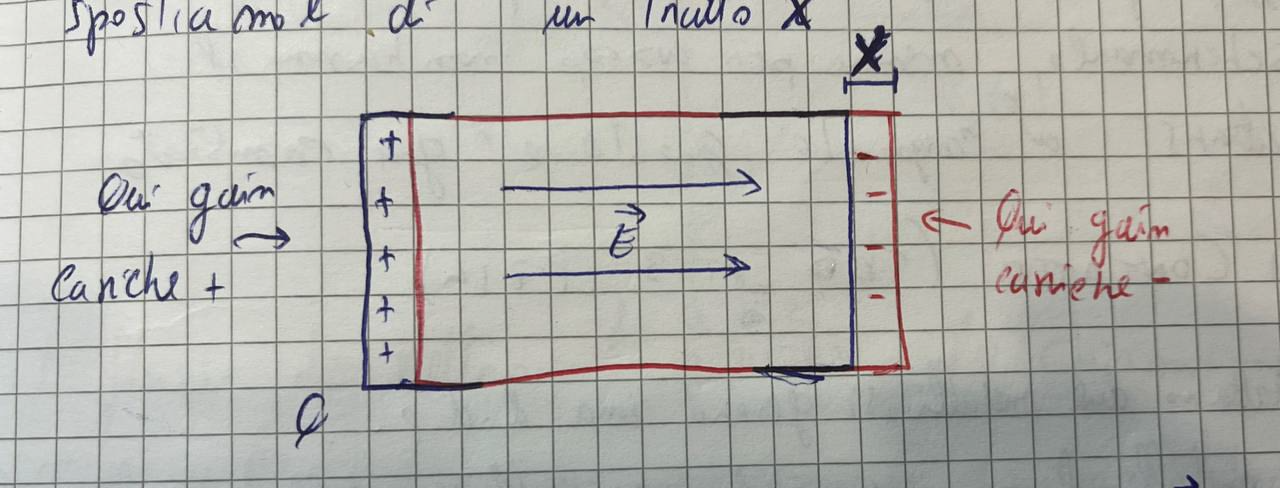
\includegraphics[width=0.75\linewidth]{img/trattoDeltaxboh.png}
    \end{figure}
    Si instaura un campo elettrico $\vec{E}$ nel materiale. La carica $Q$ accumulata ai lati è pari al prodotto fra volume e densità di carica. Se il metallo ha sezione $S$:
    $$Q = xS \cdot ne$$
    Dunque la densità di carica superficiale è:
    $$\sigma_{sup} = \frac{Q}{S} = nex$$
    Da cui, per un consdensatore a facce piane parallele:
    $$|\vec{E}| = \frac{\sigma_{sup}}{\varepsilon_{0}} = \frac{nex}{\varepsilon_{0}}$$
    Gli elettroni, che hanno verso opposto a quello del campo elettrico, vengono allora riattirati verso la zona dalla quale sono stati tolti con forza:
    $$F = m_{e}a = m_{e} \ddot{x} = - \vec{E} = -\frac{ne^{2}}{\varepsilon_{0}}x$$
    Dunque otteniamo l'espressione di un oscillatore armonico con pulsazione pari alla frequenza di plasma:
    $$\ddot{x} = -\frac{ne^{2}}{m_{e}\varepsilon_{0}}x \implies \omega ^{2} = \frac{ne^{2}}{m_{e}\varepsilon_{0}} = \omega_{p}$$
    Capiamo meglio allora perché per $\vec{E}$ a bassa si riesce ancora a schermare gli elettroni, mentre per frequenze superiori gli elettroni non hanno il tempo di adattarsi che il campo elettrico ha già cambiato verso.

    \section{Potenziali di contatto ed effetto Seebeck}
        Quando si contattano dei metalli si genera una differenza di potenziale. Un contatto per noi si ha quando due metalli formano un solo cristallo/metallo.
        Quando due metalli sono lontani (i.e. ancora non contattati) le caratteristiche nel grafico densità di stati/energia $(N(E);E)$ sono quelle solite.
        Considerati infatti due metalli con densità di stati $N_{1}(E)$ ed $N_{2}(E)$, le caratteristiche pre-contatto hanno una forma simile:
        \begin{figure}[h!]
            \centering
            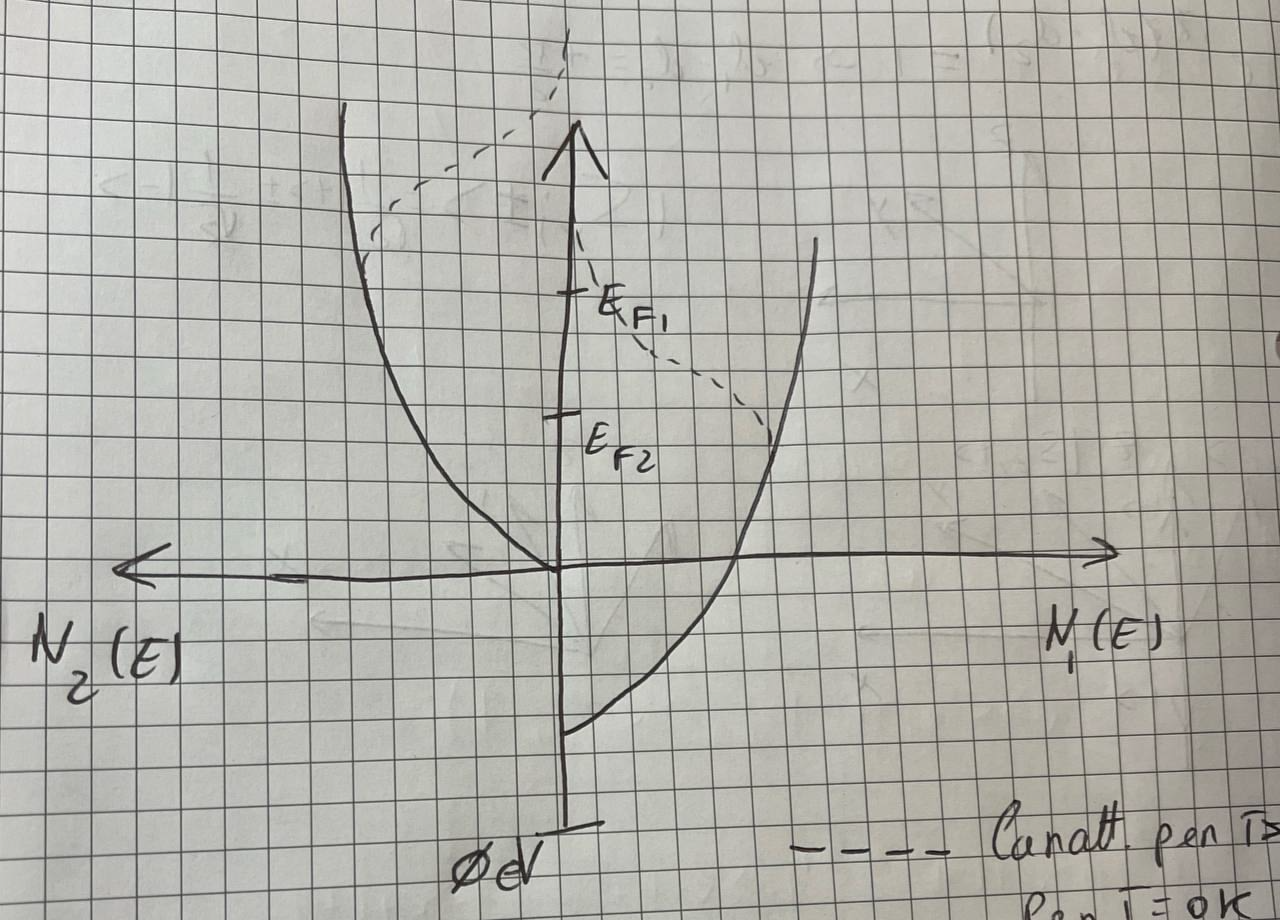
\includegraphics[width=0.5\linewidth]{img/CaratteristicaSeebeckPreContatto.png}
            \caption{Caratteristica pre-contatto: con il tratteggio è indicata la caratteristica per $T>0k$, mentre quella per $T=0K$ con il continuo.}
        \end{figure}

        Nel nostro caso, puramente a titolo d'esempio, $0<E_{F2} <E_{F1}$. Poiché i due metalli sono neutri, il potenziale di barriera è lo stesso per entrambi e vale $E_{B}$ (non mostrato in figura).\\
        A contatto avvenuto si raggiunge \textit{l'equilibrio dinamico}, condizione per la quale il flusso di elettroni netto è nullo sia da un lato della giunzione che dall'altro (i.e. il flusso che va da metallo 1 a metallo 2 è lo stesso di quello fra metallo 2 e metallo 1).
        Il flusso di elettroni per unità di volume lo chiamiamo $n_{12}(E)$.
        Tale flusso sarà proporzionale con una certa costante $A$ a quanti stati sono occupati nel metallo 1, perché se non ce ne fossero non ci sarebbe alcun flusso. Bisogna però tener conto di quanti stati disponibili ci sono nel metallo 2!\\
        Il numero di stati vuoti, se $\rho_{PIENI} = Nf$, è $\rho_{VUOTI} = N(1-f)\rho_{PIENI}$
        Dunque:
        $$n_{12} = A \rho_{1}(E)[N_{2}(E)[1-f_{2}(E)]$$
        dove abbiamo messo $f_{2}$ e non $f$ perché la funzione di Fermi Dirac dipende anche dalla temperatura e generalmente $T_{1} \neq T_{2}$.
        Espandiamo l'espressione di $\rho_{1}(E) =N_{1}(E)f_{1}(E)$ (ricordiamo, numero di stati pieni nel metallo 1) per ottenere:
        $$n_{12} = AN_{1}(E)f_{1}(E)N_{2}(E)[1-f_{2}(E)]$$
        Il flusso opposto sarà $n_{21}$ che sarà esattamente speculare ad $n_{12}$:
        $$n_{21} = AN_{2}(E)f_{2}(E)N_{1}(E)[1-f_{1}(E)]$$
        Allora eguagliando i due flussi, la condizione di equilibrio dinamico la si ha per:
        $$f_{1} = f_{2}$$
        cioè quando le funzioni di Fermi-Dirac sono uguali, condizione soddisfatta per:
        $$\begin{cases}
            E_{F1} = E_{F2} \\
            T_{1} = T_{2}
        \end{cases}$$
        Il salto di energia $\Delta E$ per traslare il grafico del metallo 2 sarà:
        $$\Delta E = (E_{B2} - E_{F2})-(E_{B1} - E_{F1}) = E_{W2} - E_{W1}$$
        cioè il potenziale di estrazione netto fra i due metalli. Ora che ci siamo spostai, è cambiata la barriera di energia $E_{B1}$, che viene traslata di $\Delta E$.\\
        La quantità $\Delta E$ si chiama \textbf{potenziale di contatto}.\\
        \newpage
        Se questi sono i due metalli in 4K UHD:
        \begin{figure}[h!]
            \centering
            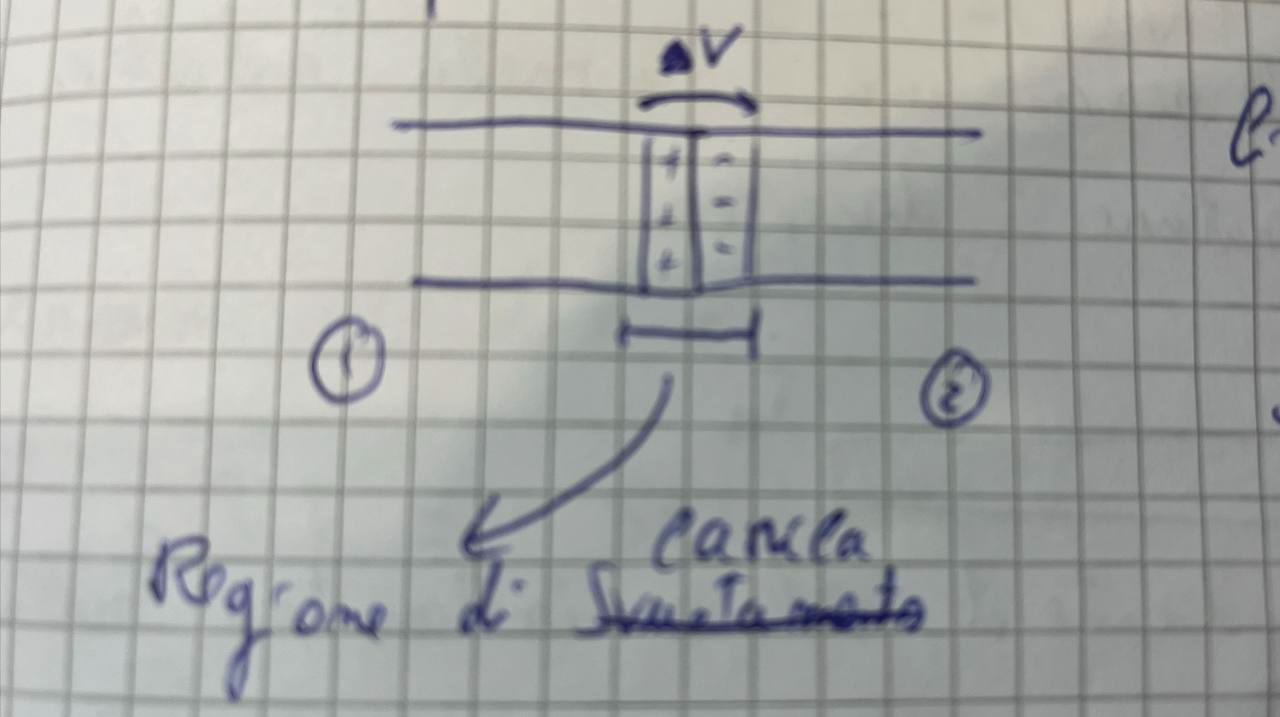
\includegraphics[width=0.75\linewidth]{img/metal1.png}
        \end{figure}
        Quanto valgono i fluessi di elettroni che lo attraversano? Quanto è larga la regione di carica? Descriviamolo come se fosse un condensatore ed assumiamo, per semplicità, che lo spesso delle zona di carica positiva e negativa valgano entrambe $d$. Se $S$ è la sezione dei due metalli, risulta:
        $$\begin{cases} 
            Q = ned \cdot S \\
            C = \displaystyle \frac{Q}{\Delta V} = \frac{\varepsilon_{0}S}{d}
        \end{cases}$$
        da cui si ricava $d$:
        $$d = \sqrt{\frac{\varepsilon_{0}\Delta V}{ne}}$$
        Se $n \simeq 10^{28}, \quad \Delta V \sim 1V$ risulta $d \simeq$\si{\angstrom}. Tale regione è molto molto ristretta e tale sarà anche la carica.
        \paragraph{}
            Parliamo allora di effetto Seebeck. Consideriamo una sbarretta metalicca con ai suoi capi due temperature diverse, $T_{A}$ e $T_{B}$. Per effetto del gradiente di calore instauratosi nella sbarretta, si genera una differenza di potenziale ai suoi capi.\\
            Quello che accade fisicamente è che gli elettroni nel punto A si muovono casualmente, così come in B, a velocità maggiori di quelli nel punto B, in quanto $T_{A}>T_{B}$.\\
            Statisticamente, guardando la figura, ci saranno tanti elettroni che vanno da A a B quanto sono quelli che vanno da B ad A. I primi hanno velocità maggiore dei secondi e dunque c'è uno spostamento netto di elettroni con velocità netta pari alla differenza delle velocità dei due gruppi di elettroni. Allora si instaura un campo elettrico $\vec{E}$ in virtù dell'accumulo di carica negativa in B, che porta dopo un po' alla stazionarietà.
            \begin{figure}[h!]
                \centering
                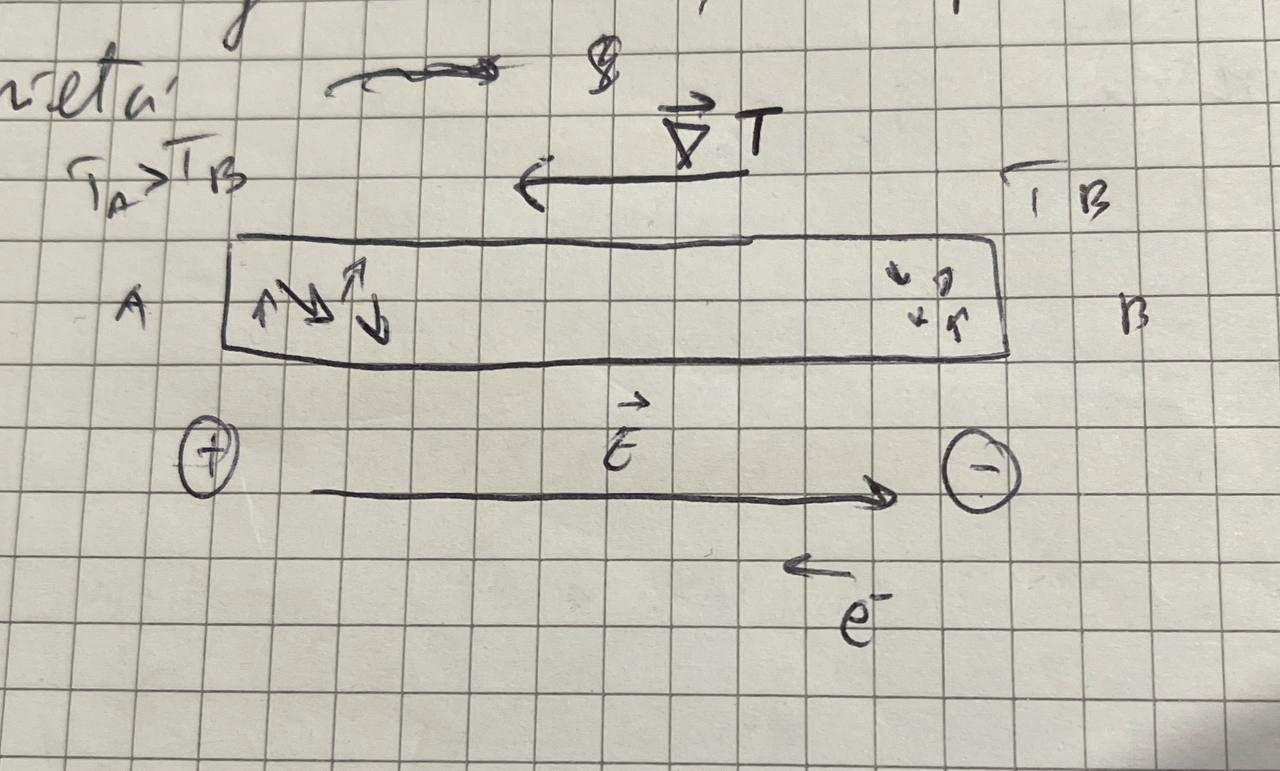
\includegraphics[width=0.5\linewidth]{img/asset1.png}
            \end{figure}
            Quello che si osserva è che $\vec{E} \propto \vec{\nabla} T$ con un certo coefficiente $S(T)$:
            $$\vec{E} = - S(T)\vec{\nabla}T$$
            detto \textbf{coefficiente di Seebeck}, il quale dipende dalla temperatura e ha le dimensioni di un campo elettrico su una temperatura, dunque $V \cdot m \cdot K^{-1}$.
            In termini di differenza di potenziale:
            $$\vec{E} =- \vec{\nabla}V = -S(T) \vec{\nabla}T$$
            che in una dimensione diventa:
            $$- \frac{\partial V}{\partial x} = - S(T) \frac{\partial T}{\partial x} \implies dV = S(T)dT$$
            dunque per ricavare la differenza di potenziale ai capi della sbarretta basta integrare in $[T_{2},T_{1}]$:
            $$\Delta V = \int_{T_{1}} ^{T_{2}} S(T)dT$$
            Consideriamo di nuovo una sbarretta di metallo con libero cammino medio e consideriamo un punto $x$ qualsiasi della sbarretta:
            \begin{figure}[h!]
                \centering
                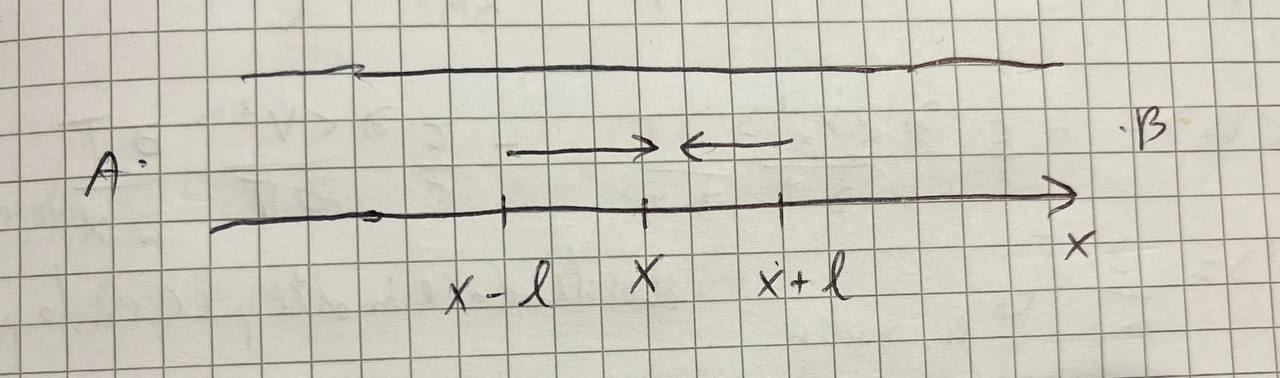
\includegraphics[width=0.5\linewidth]{img/sbarrettapt2.png}
            \end{figure}
            Detta $v_{x}$ la velocità lungo $x_{1}$, questa è funzione di $T$ che a sua volta è funzione di $x$:
            $$v_{x} = v_{x}(T(x))$$
            Vogliamo valutare la velocità netta $v_{T}$ come media della velocità degli elettroni che provengono da A e quella di quelli che provengono da B:
            $$v_{T} = \frac{1}{2} [v_{x}(T(x-l))-v_{x}(T(x+l))]$$
            Sviluppiamo con taylor in $l=0$ per $x$:
            $$v_{T} \simeq \frac{1}{2} [(v_{x}(T(x))+(-l)\frac{\partial v_{x}}{\partial T} \cdot \frac{\partial T}{\partial x})-(v_{x}(T(x))+l \frac{\partial v_{x}}{\partial T} \frac{\partial T}{\partial x})] = -l \frac{\partial v_{x}}{\partial T} \frac{\partial T}{\partial x}$$
            Ricordando che $l=v_{x}\tau$:
            $$\displaystyle v_{x}\tau \frac{\partial v_{x}}{\partial T} = \frac{\partial}{\partial T} (\frac{\tau}{2}\frac{\partial v_{x} ^{2}}{\partial T}) = -v_{x}\tau \frac{\partial v_{x}}{\partial T} \frac{\partial T}{\partial x} = -\frac{\tau}{2} \frac{\partial ^{2}v_{x}}{\partial T} \frac{\partial T}{\partial x}$$
            Valutiamo la media $\braket{v_{T}}$ e teniamo presente che:
            $$\braket{v_{x} ^{2}} = \frac{\braket{v_{x}}}{3}$$ perché $\braket{v^{2}} = \braket{v_{x}^{2}}+\braket{v_{y}^{2}}+\braket{v_{z} ^{2}}$ ed ipotizziamo ragionevolmente che sulle tre direzioni spaziali le componenti della velocità quadratica media siano ugual.
            Dunque:
            $$\braket{v_{T}} = -\frac{\tau}{2} \frac{\partial \braket{v_{x} ^{2}}}{\partial T} \frac{\partial T}{\partial x} = - \frac{\tau}{6} \frac{\partial \braket{v ^{2}}}{\partial T}$$
            Poiché $\braket{v^{2}} = \displaystyle  \frac{2}{m_{e}} \bar{E}$, con $\bar{E}$ energia media, dividendo e moltiplicando per $m_{e}/2$ si ottiene:
            $$-\frac{\tau}{3m_{e}} \cdot \frac{m_{e}}{2} \frac{\partial \braket{v^{2}}}{\partial T} \frac{\partial T}{\partial x} = - \frac{\tau}{2m_{e}} \frac{\partial \bar{E}}{\partial t} \frac{\partial T}{\partial x}$$
            Moltiplicando e dividendo per $n$, la densità di elettroni, poiché la capacità termica per unità di volume è $\displaystyle n \frac{\partial E}{\partial T}$:
            $$= - \frac{\tau C_{el}}{3n m_{e}} \frac{\partial T}{\partial x} = \braket{v_{T}}$$
            Per passare all'espressione del campo elettrico, teniamo presente che la stazionarietà è raggiunta quando la velocità di deriva $\vec{v}_{m}$ eguaglia $\braket{v_{T}}$. Ragionando sempre in una dimensione:
            $$v_{m} = - \mu_{n}E_{x} = -\braket{v_{T}} = \frac{\tau C_{el}}{3nm_{e}}\frac{\partial T}{\partial x} \implies E_{x} = - \frac{\tau  C_{el}}{3\mu n m_{e}} \frac{\partial T}{\partial x}$$
            poiché $\displaystyle \mu_{n} = \frac{e \tau}{m_{e}}$, allora:
            $$E_{x} = - \frac{C_{el}}{3ne} \frac{\partial T}{\partial x}$$
            In definita ricaviamo per confronto l'espressione del cofficiente di Seebeck:
            $$S(T) = \frac{C_{el}}{3ne} = \frac{\pi^{2}}{6} \frac{k_{B}}{e} (\frac{k_{B}T}{E_{F}})$$
            avendo sostituito l'espressione della capacità termica elettronica ricavata nel precedente capitolo. In termini di potenziale:
            $$\Delta V = \int_{T_{1}} ^{T_{2}} \frac{C_{el}}{3ne} dT$$
    \section{Conducibilità termica elettronica}
        Consideriamo la stessa sbarretta di prima, con temperature $T_{A}$ e $T_{B}$ ai suoi capi. Al flusso degli elettroni è associato un flusso di energia, in quanto ognuno trasporta la propria energia cintetica. Il contributo ionico al trasporto di calore è \textbf{nullo}, nel modello di Sommerfeld non prevede ioni. In questo caso il contributo $k_{T}$ è puramente elettronico. Il flusso di energia associato al moto degli elettroni è:
        $$\vec{J}_{a} = n\bar{E} \braket{\vec{v}}$$
        In una dimensione:
        $$J_{Q} = nev_{x}$$
        Consideriamo sempre la situazione dove ci sono due flussi elettronici, uno da destra e l'altro da sinistra, per i quali prima abbiamo calcolato $\braket{v_{T}}$. Calcoliamo ora l'energia media $\bar{E}$ sulla falsariga del procedimento di prima:
        $$\bar{E}_{T} = \frac{1}{2} [\bar{E}(T(x-l))-E(T(x+l))]$$
        da cui si ricava facendo lo sviluppo e compagnia:
        $$k_{T} = \frac{n \braket{v^{2}} \tau}{3}C_{el}$$
        La conducibilità termica è definita come:
        $$\vec{J}_{a} = -k_{T} \vec{\nabla}T$$
        dunque sostituendo si ottiene, in una dimensione:
        $$\vec{J}_{a} = - \frac{\braket{v^{2}}\tau}{3}C_{el} \frac{\partial T}{\partial x} \simeq - \frac{v_{F} \tau}{3} C_{el} \frac{\partial T}{\partial x} $$
        perché in un metallo $\braket{v^{2}} \simeq v_{F} ^{2}$.\\
        Come prima, sostituendo l'espressione di $C_{el}$ si ricava la \textbf{legge di Wiedman-Franz}:
        $$k_{T} = \frac{\pi ^{2}}{3} \frac{k_{b} ^{2}}{e^{2}} \sigma T = L \sigma T$$
        dove $L = \displaystyle \frac{\pi}{3} \frac{k_{b} ^{2}}{e^{2}}$ è detto \textit{numero di Lorentz}.
    \section{Tecniche LEED e RHEED}
        \paragraph{}
            Quando un elettrone si comporta come un onda, valgono le relazioni di De Broglie:
            $$\begin{cases}
                \nu = E/h \\
                \lambda = h/p
            \end{cases}$$
        Facendo le funny sostituzioni si ricava l'energia e la funzione d'onda in nanometri:
        $$\begin{cases}
            E = \displaystyle \frac{p^{2}}{2m_{e}} = \frac{h^{2}}{\lambda ^{2}2m_{e}} \\
            \lambda = \displaystyle \frac{h}{\sqrt{2m_{e}E}} = \frac{1.22 \textrm{nm}}{(E[eV])^{1/2}}
        \end{cases}$$
        Gli acronimi LEED e RHEED stanno rispettivamente per \textit{Low Energy Electron Diffraction} ed \textit{Reflection High Eergy Electron Diffraction} le lunghezze d'onda devono essere comparabili con i passi reticolari.\\
        Per la tecnica LEED le energie sono nell'ordine delle decine alle centinaia di elettronVolt, indi per cui c'è minima prenotazione degli elettroni nella materia, nell'ordine degli \si{\angstrom}ngstrom, e ragion per la quale la tecnica LEED è una \textbf{tecnica di indagine superficiale}.\\
        A queste energie il fenomeno di \textit{back-scattering}, per il quale gli elettroni si diffondono all'indietro, è comune. Si piazza allora il cannone elettronico in modo da misurare la differenza di cammino fra le backscatterate (Treccani '25):
        \begin{figure}
            \centering
            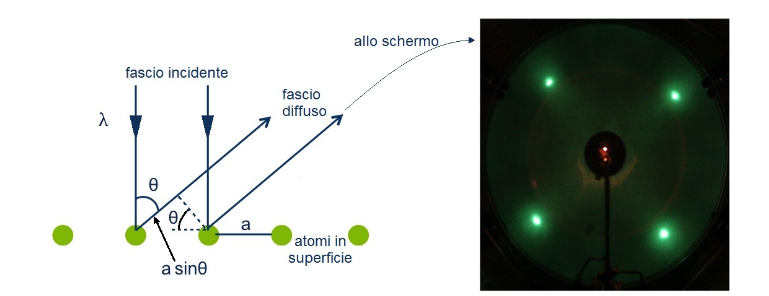
\includegraphics[width=0.5\linewidth]{img/LEED2.png}
            \caption{I fasci elettronici incidono la superficie del cristallo}
            \label{fig:enter-label}
        \end{figure}
        \begin{figure}[h!]
            \centering
            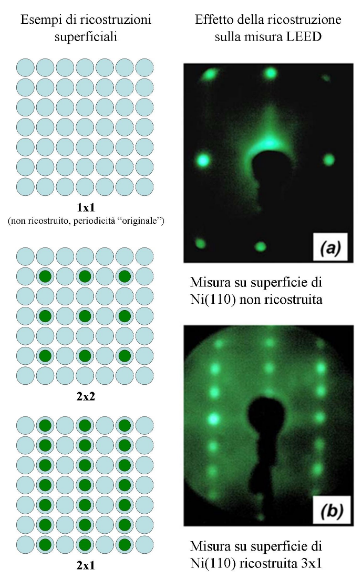
\includegraphics[width=0.35\linewidth]{img/LEED.png}
            \caption{Notare il cannone quasi perpendicolare alla superficie del cristallo per via del backscattering}
        \end{figure}\newpage
        Deve valore Bragg e dunque $a \sin{(\vartheta)} = n \lambda$ affinché ci sia un massimo. Per la LEED occorre la camera a vuoto ove i raggi vengono assorbiti in aria normale, a differenza dei raggi X.\\
        Lo schermo individua dei massimi di diffusione per quei valori di $\vartheta$ che verificano le condizioni di Bragg. Dunque ciò che si vede sullo schermo è il reticolo reciproco, tipicamente per $n=1$ perché è comicamente stretto. Nella figura, anche se si vede poco, ci sono dei pattern che si ripetono con spaziature più strette rispetto a quelle del reticolo in esame, dette "sovrastrutture superficiali" ed ascrivibili ad una differente organizzazione della superficie più esterna del cristallo, assieme all'eventuale assorbimento di specie chimiche varie. Il libero cammino medio è sensibile all'energia degli elettroni nel cristallo, ragion per la quale vengono scelti per il LEED energie sui $100eV$, cosicchè gli atomi vengono fermati quanto più in superficie possibile. \textbf{DA FINIRE CON RHEED}

\chapter{Vibrazioni reticolare in un solido cristallino e Modello di Debye}
    \section{Vibrazioni in una dimensione}
        \paragraph{}
        Gli atomi vibrano attorno alla loro posizioni di equilibrio. Molte lezioni fa approssimammo con Taylor, troncando al II ordine, l'energia di interazione:
        $$U(x) = U(0)+\frac{1}{2}\beta x^{2}$$
        che assume comportamento elastico valido per piccole oscillazioni.\\
        Vogliamo descrivere il comportamento degli atomi come se fosse quello di un oscillatore aromnico. Ragioneremo prima in una dimensione per poi generalizzare al caso tridimensionale. Partiamo da una catena di $N$ atomi uguali ed equispaziati:
        \begin{figure}[h!]
            \centering
            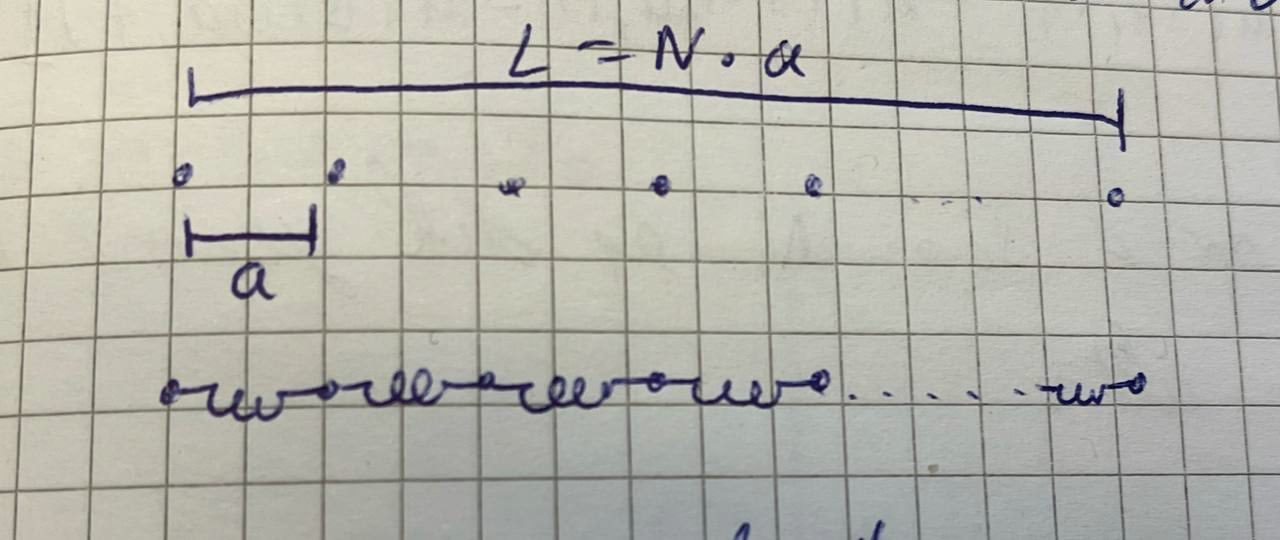
\includegraphics[width=0.5\linewidth]{img/imnothere.png}
        \end{figure}
        Ipotizziamo che ogni atomo interagisca con i suoi primi vicini in modo elastico. Quando gli atomi sono nelle loro posizioni di equilibrio, cioè per $x=R-R_{0} = 0$, non c'è alcuna interazione elastica in quanto le molle sono rilassate. Indichiamo gli atomi con l'indice $s$ che varia da $0$ ad $N-1$, mentre la loro posizione sull'asse $x$ sarà $x=sa$.
        \begin{figure}[h!]
            \centering
            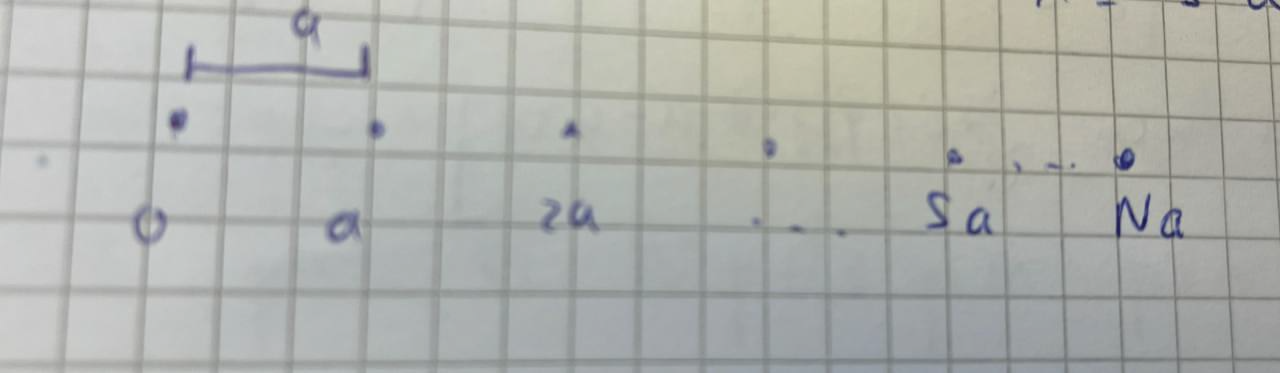
\includegraphics[width=0.5\linewidth]{img/imnothere2.png}
        \end{figure}
        Indichiamo con $u$ lo spostamento dell'atomo rispetto alla propria posizione di equilibrio:
        $$u = u(sa, t)$$
        la quale dipende sia dal tempo che dalla posizione $sa$ dell'atomo.\\
        La forza esercitata sull'atomo (verso destra) sarà somma dei contributi da destra e sinistra, presi con il verso negativo per comodità (basta verificare la forza presa con il verso positivo vada dall'atomo prima a quello dopo):
        $$M \ddot{u} (sa, t) = -\beta [u(sa,t)-u((s-1)a,t)]-\beta [u(sa,t)-u(s+1)a,t)]$$
        I termini con $x=(s+1)a$ ed $x=(s-1)a$ tengono contro del fatto che gli estremi della molla a destra e asinistra non sono fissi e dipendono dagli spostamenti dei primi vicini rispetto all'equilibrio.\\
        Segue:
        $$M\ddot{u}(sa,t) = - \beta [2u(sa,t) -u((s-1)a,t)-u((s+a)a,t)]$$
        Per $N$ atomi ci sono $N$ equazioni del genere e sono l'una dipendenti dalle altre.\\
        Proviamo a cercare una soluzione del tipo onda piana:
        $$u(sa,t) = u_{0}\exp{(-i(qsa-\omega t))}$$
        Sostituiamo e vediamo per quali $q$ ed $\omega$ vale:
        $$-\omega ^{2} M u_{0} \exp{(-i(qsa-\omega t))}=$$
        $$ =\beta u_{0}[2\exp{(-i(qsa-\omega t))}-\exp{(-i(q(s+1)sa-\omega t))}-\exp{(-i(q(s+1)a-\omega t))}]$$
        Il secondo membro lo riscriviamo come:
        $$- \beta u_{0}\exp[{-i(qsa-\omega t)}] (2-\exp{[iqa]}-\exp{[-iqa]})$$
        e dunque:
        $$\omega^{2}M = -2\beta [1-\cos{8qa)} \implies \frac{4\beta}{M}\sin^{2}(\frac{qa}{2})= \omega ^{2}$$
        L'ultimo passaggio è giustificato dalle formule di bisezione.\\
        Dunque un'onda piana è soluzione solo se vale:
        $$\omega(q) = 2 \sqrt{\frac{\beta}{M}}|\sin{(\frac{qa}{2})}|$$
        Per noi è significativo, piuttosto che la $v_{fase} = \omega/q$, la velocità di gruppo:
        $$v(q) = \frac{d \omega(q)}{dq} \implies |v(q)|=a \frac{\beta}{M}|\cos{(\frac{qa}{2})}|$$
        \begin{figure}[h!]
            \centering
            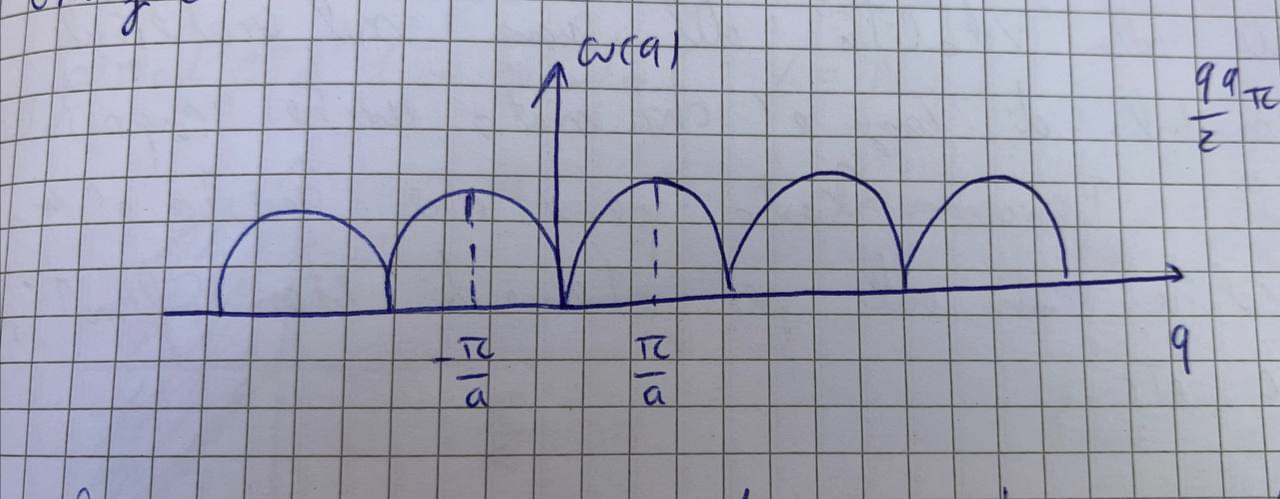
\includegraphics[width=0.5\linewidth]{img/imnothere3.png}
        \end{figure}
        Graficando la $\omega(q)$ ci si rende conto che essa è periodica di $\displaystyle\frac{2\pi}{a}$, in quanto $qa/2 = \pi$. In una dimensione la zona $[-\pi/2, \pi/2]$ è la \textit{prima zona di Brillouin}. Dalla periodicità della funzione è allora possibile studiarla nella zona di Brillouin, estendendone poi i risultati ovunque.\\
        Anche la $u(sa,t)$ è periodica di $2\pi/a$ quindi stesso discorso. Se ci si mette ben dentro la zona di Brillouin, cioè per $q << \pi/a$, la $\omega(q)$ è circa lineare e può essere approssimata ad:
        $$\omega(q) \simeq a \sqrt{\frac{\beta}{M}} \implies v(q) = \simeq a \sqrt{\frac{\beta}{M}}$$
        C'è una relazione anche con $E$ ,il modulo di Young, che abbiamo citato in precedenza. Esso dipende solo dal materiale:
        $$E = \frac{N'}{S}a\beta = \frac{1}{a}\beta$$
        perché $\beta = aE$ per un reticolo cubico.
        L'ultimo membro si ottiene per un reticolo cubico, la cui superficie è $S=a^{2}$ e ad ogni cella è associato un solo atomo $(N'=1)$. \\
        La velocità $v(q)$ che abbiamo trovato prima allora vale (sempre per un reticolo cubico):
        $$v(q) = a \sqrt{\frac{\beta}{M}} = \sqrt{\frac{a^{3}E}{M}} = \sqrt{\frac{E}{\rho}}$$
        dove $\rho$ è la densità del materiale ed $M$ la massa atomica.\\
        La $v(q)$ corrisponde alla velocità del suono nel materiale. Il modulo di Young è chiamato andche \textit{compressibilità del materiale}. Teniamo conto che però questo è un caso particolare, che vale per catene di atomi infiniti all'interno di un reticolo cubico.

        \paragraph{}
            Come ordine di grandezza:
            $$\omega_{m} = 2 \sqrt{\frac{\beta}{M}} \simeq 10^{13} \div 10^{14}$$
            che in energia corrisponde ad $\hbar \omega_{m} \simeq 10^{-2} \div 10^{-3} eV$.
            Cosa cambia per una catena di atomi \textit{finita?}\\
            Precisiamo prima che la funzione $u(x,t)$ descrive il profilo dell'onda e non la posizione dell'atomo, quindi quantifica quanto gli atomi si spostano dalla loro posizione d'equilibrio.\\
            Ipotizziamo che primo e ultimo atomo siano fermi, cioè:
            $$u(0,t) = u(Na,t) = 0$$
            Poiché $Na = L$ (lunghezza del materiale) ed
            $$u(sa,t) = u_{0}\exp{[-i(qsa-\omega t)]} = u_{0}\sin{(q_{n}sa)}\exp{[i\omega t]}$$
            la condizione affinché il seno si annulli agli estremi è che sia periodico di: 
            $$q_{n}sa = n \pi \implies q_{n} = \frac{n \pi}{L}$$
            Ciò equivale, al contorno, ad ammettere soltanto alcuni modi di oscillazione, cioé solo alcuni valori di $q_{n}$. Ci sono $N$ modi di oscillazione indipendenti, mentre gli altri si ripetono per periodicità, in quanto $L=Na$.\\
            Dunque possiamo ricavare i valori massimi e minimi di lunghezze d'onda, assunte rispettivamente per $x=0$ ed $x=L$:
            $$q_{min} = \frac{\pi}{L} \implies\lambda_{max} = \frac{2\pi}{q_{min}}$$
            $$q_{max} = \frac{N \pi}{L} \implies \lambda_{min} = 2a$$
            Ipotizziamo  ora che nela catena ci siano più atomi diversi. Bisogna scrivere un set di equazioni per ogni gruppo di atomi di un certo tipo (sempre ragionando in una dimensione).\\
            Questi ovviamente possono comportarsi come vogliono. Potrebbero, ad esempio, essere in fase tra di loro e disporsi su diversi valori della funzione $u(x,t)$:
            \begin{figure}[h!]
                \centering
                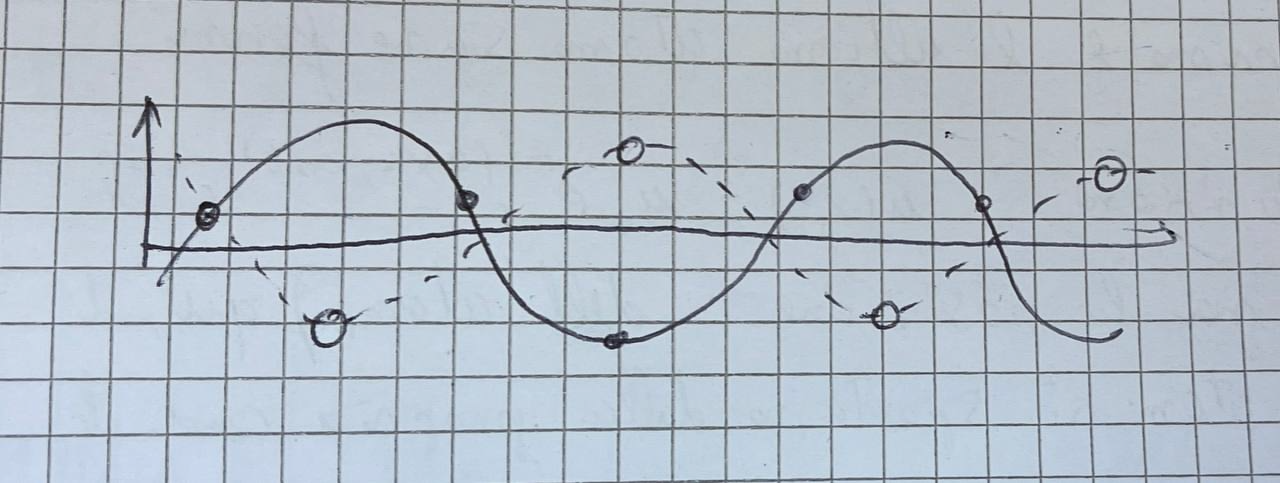
\includegraphics[width=0.5\linewidth]{img/imnothere5.png}
                \caption{Atomi neri e atomi bianchi sono due specie atomiche diverse}
            \end{figure}
            Dalla figura si intuisce che ci sono diversi modi di oscillazione: per esempio gli atomi nei pressi dei minimi della funzioni oscilleranno molto più di quelli in prossimità dell'asse delle ordinate.\\
            Quando gli atomi di specie diversa oscillano \textit{in fase} allora il moto di oscillazione viene detto \textbf{acustico}, mentre in controfase viene detto \textbf{ottico}.\\
            Graficando la situazione:
            \begin{figure}[h!]
                \centering
                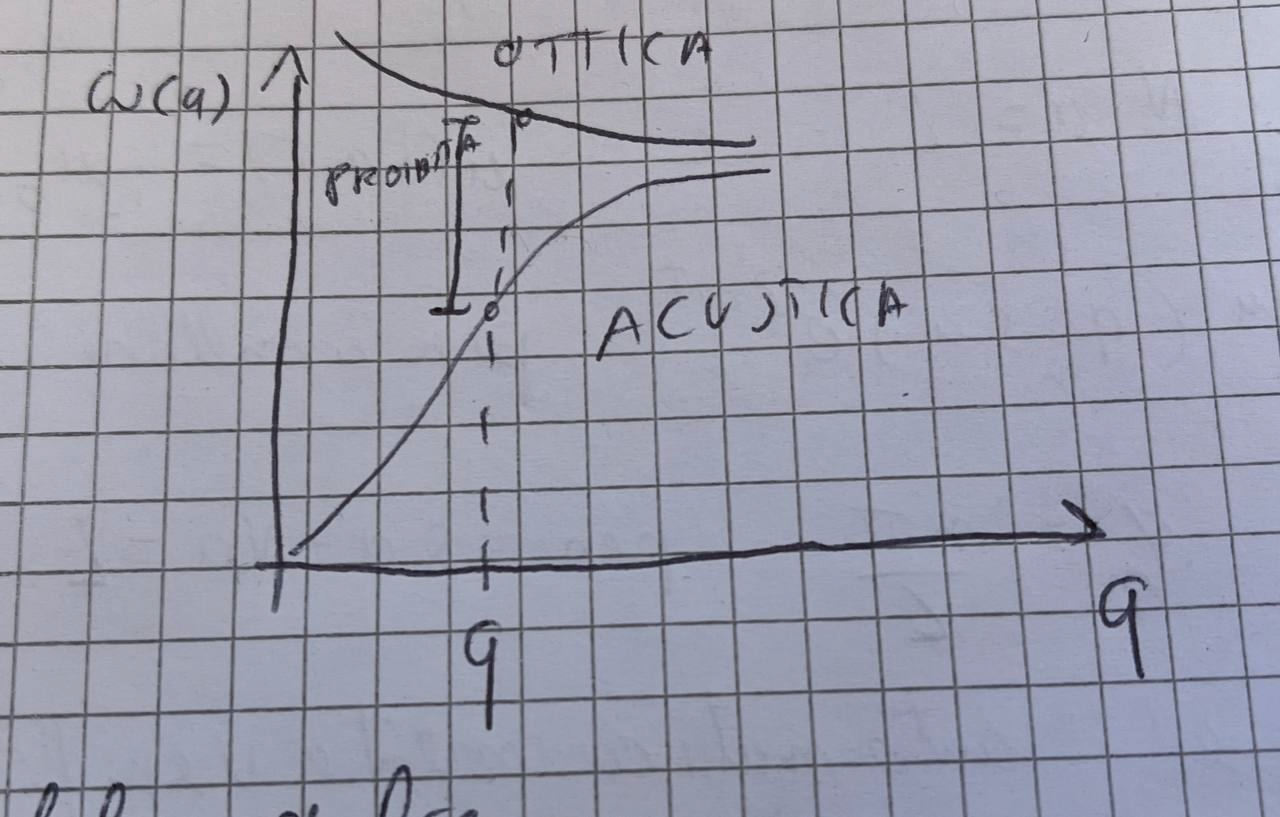
\includegraphics[width=0.5\linewidth]{img/imnothere6.png}
            \end{figure}
            Per ogni $q$, si vede dal grafico, esiste un valore di $\omega(q)$ presente o in banda ottica o in acustica, oppure in entrambe. I valori in mezzo costituiscono la \textbf{banda proibita}.
            \paragraph{}
            Possiamo ora generalizzare al caso tridimensionale. Definendo:
            $$q_{nj} = n_{j}\frac{\pi}{L_{j}}$$
            con $j \in \{x, y, z\}$ ed $n_{j} \in [0, N_{j}]$, dove $N_{j}$ è il numero di atomi lungo l'asse $\hat{j}$.
            Ci sono allora $N_{z}N_{x}N_{y}$ valori possibili di $\vec{q}$, che ora è un vettore (giustamente) tridimensionale:
            $$\vec{q} = (q_{x}, \ q_{y}, \ q_{z})$$
            I modi di oscillazione stavolta sono $3N_{j}$ e non $N_{j}$, perché possono essere anche trasversali o longirudinali per ogni valore di $\vec{q}$. La $\omega(\vec{q})$ risulta comunque periodica nel reticolo reicproco, cioè tale per cui:
            $$\omega (\vec{q}) = \omega(\vec{q} + \vec{G})$$

    \section{Densità di modi}
            Vogliamo trovare un'espressione per ricavare il numero di modi relativo ad un valore di $\vec{q}$ fissato, un po' come abbiamo fatto per gli stati nel modello di Sommerfeld.Identifichiamo il modo in tre dimensioni come:
            $$q_{n_{x},n_{y},n_{z}} = n_{x,y,z}\frac{\pi}{L_{x,y,z}}$$
            Sia $\Delta ' (q)$ la funzione che ci dice quanti modi cadono nella sfera di raggio $q$. Nello spazio $q$ tali modi sono equispaziati e ad ognuno "affidano" un volumetto $ \displaystyle (\frac{\pi}{L})^{3}$, assumendo per semplicità $L_{x}=L_{z}=L_{y} = L$.
            Allora il numero di volumetti sarà:
            $$D '(q) = \frac{4}{3} \pi q^{3} (\frac{1}{(\frac{\pi}{L})^{3}}) \frac{1}{8} \cdot 3$$
            dove $1/8$ e $3$ tengono conto del fatto che in 3D solo il primo ottante è indipendente e ci sono 3 modi di oscillazione per ogni valore di $\vec{q}$.
            Si ricava, infine:
            $$D ' (q) = \frac{q^{3}L^{3}}{2 \pi^{2}} = \frac{q^{3}V}{2 \pi^{2}}$$
            La generalizzazione di questa quantità (senza apice) valutata per unità di volume è:
            $$D(q) = \frac{q^{3}}{2 \pi}$$

            Operiamo quella che viene detta \textit{approssimazione di Debye}: assumiamo che la relazione tra $\omega$ e $q$ sia lineare:
            $$\omega  = v_{0}q$$
            dove $v_{0}$ è la velocità del suono nel materiale e viene assunta costante per tutti i modi. Risulta allora, dall'espressione della quantità di modi per unità di volume, sostituendo $q = \omega/v_{0}$:
            $$D (\omega) = \frac{\omega ^{3}}{2 \pi ^{2}v_{0}^{3}}$$
            Questa relazione vale fino ad un certo valore massimo di frequenza $\omega_{D}$, detta \textbf{frequenza di Debye}, che per la $D(\omega)$ ha un significato simile a quello che aveva $E_{F}$ per la $N(E)$ nel modello di Sommerfeld.\\
            In questo caso la $D(\omega_{D})$ corrisponde al numero totale di modi per unità di volume. La densità di atomi per unità di volume la chiamiamo $n_{a}$, mentre la $n_{e}$ è la quella di elettroni.\\
            Sopra la $\omega_{D}$ \textbf{non} ci sono modi di oscillazione e questa è una differenza sostanziale per la $E_{F}$ rispetto alla $N(E)$, che a temperature non nulle può avere stati al di sopra di essa.\\
            Dunque:
            $$D(\omega_{D}) = \frac{\omega_{D} ^{3}}{2 \pi^{2}v_{0} ^{3}} = \frac{3N}{V} = 2n_{a}$$
            da cui:
            $$\omega_{D} = (6 \pi^{2}n_{a})^{1/3}v_{0}$$
            Notiamo che la $\omega_{D}$ dipende dalla densità di stati e dalla velocità del suono nel materiale. Analogamente a quando trattammo il modello di Sommerfeld, definendo il momento di Fermi, si può definire il \textbf{momento di Debye} $q_{d}$ per il quale si ottiene $\omega_{D}$:
            $$q_{D} = \omega_{D}/v_{0} = (6 \pi^{2}n_{a})^{1/3}$$
            Per gli ordini di grandezza, se $n_{a} \simeq 10^{28}m^{-3}, \ v_{0} \simeq 10^{3}m/s$ si ottiene $q \simeq 1$\si{\angstrom}$^{-1}$
            Analogamente, si definisce una temperatura di Debye $\vartheta_{D} = \hbar \omega_{D}/k_{B}$.
            Definiamo la \textit{densità di modi} $F(\omega)$ tale per cui:
            $$D(\omega= = \int_{0} ^{\omega} F(\omega ')d \omega '$$
            da cui si ricava:
            $$F(\omega) = \frac{d D(\omega)}{d \omega} = \frac{d}{d\omega} (\frac{\omega ^{3}}{2 \pi^{2}v_{0}^{3}}) = \frac{3 \omega ^{2}}{2 \pi^{2}v_{0} ^{3}}$$
            la quale vale per $\omega \leq \omega_{D}$.
            L'energia (quantizzata) associata alla vibrazione del reticolo è:
            $$E(\omega ) = n(\omega) \hbar \omega$$
            in questo caso trattiamo questi quanti di energia come associati al suono, detti \textbf{fononi}.\\
            Il numero di fononi non è fissato ma varia in funzione di quanto vibra il reticolo. La funzione $n(\omega, T)$ che fornisce il numero di fononi a frequenza $\omega$ e temperatura $T$ è:
            $$n(\omega, T) = \frac{1}{\exp{[\frac{\hbar \omega}{k_{B}T}]}-1}$$
            che è la funzione di \textbf{Bose-Einsten}. I fononi infatti, contrariamente agli elettroni che sono fermioni (particelle a spin semintero), sono bosoni (particelle a spin intero) per i quale non vale il principio di Pauli.\\
            Per $T \to \infty \implies k_{B}T \geq \hbar \omega_{D} \implies T \geq \vartheta_{D}$, dunque si può approssimare:
            $$n(\omega, T) \simeq \frac{1}{1 - \frac{\hbar \omega}{k_{B}T} -1} = \frac{k_{B}T}{\hbar \omega}$$
            che in termini di energia equivale ad:
            $$E(\omega) = n \hbar \omega = n \hbar \frac{k_{B}T}{\hbar \omega} = k_{B}T$$
            Moltiplicando $F(\omega)$ per $n)\omega, T)$ ed integrando:
            $$\int_{0} ^{\omega} n(\omega, T) F(\omega) d \omega = n_{ph}(T)$$
            che è il numero totale di fononi a temperatura $T$.\\
            Sostituendo la definizione di $n(\omega, T)$:
            $$n_{ph} = \frac{3}{2 \pi^{2} v_{0} ^{3}} \int_{0} ^{\omega_[D} \frac{\omega}{\exp{[\frac{\hbar \omega}{k_{B}T}]}-1}d\omega$$
            $$\frac{\hbar \omega}{K_{B}T} = x \implies \omega^{2} = (\frac{k_{B}T}{\hbar})^{2}x^{2} \implies d \omega = \frac{k_{B}T}{\hbar} dx$$
            Allora si ottiene, tenendo conto che $\omega = \omega_{D} \implies x = \hbar \omega_{D}/k_{B}T = \vartheta_{D}/T$:
            $$n_{ph} = \frac{3}{2 \pi^{2}v_{0} ^{3}} \frac{k_{B} ^{3}T^{3}}{\hbar ^{3}} \int_{0} ^{\vartheta_{D}/T} \frac{x^{2}}{e^{x}-1}dx = 9n_{a}(\frac{T^{3}}{\vartheta_{D} ^{3}}) \int_{0} ^{\vartheta_{D}/T}  \frac{x^{2}}{e^{x}-1}dx$$
            Per $T >> \vartheta_{D} \implies e^{x} \sim 1+x$
            Allora:
            $$n_{ph}(T) = 9n_{a} (\frac{T}{\vartheta_{D}})^{3} \int_{0} ^{\vartheta_{D}/T} xdx = \frac{9}{2}n_{a} (\frac{T}{\vartheta_{D}})^{3}(\frac{\vartheta_{D}}{T})^{2} = \frac{9}{2} n_{a}\frac{T}{\vartheta_{D}}$$
            dunque l'espressione del numero totale di fononi è lineare in $T$.
            Nel caso in cui $T << \vartheta_{D}$ si ottiene un risultato che riportiamo già fatto, pari a circa:
            $$n_{ph}(T) \simeq 21.2n_{a}\frac{T^{3}}{\vartheta_{D} ^{3}}$$
            Ricaviamo allo stesso modo l'energia associata alle vibrazioni reticolari:
            $$E_{ph}(T) = \int_{0} ^{\omega_{D}} n(\omega, T) \hbar \omega F(\omega)dw = \frac{3 \hbar}{2 \pi^{2}v_{0}}\int_{0} ^{\omega_{D}} \frac{\omega ^{3}}{\exp{[\frac{\hbar \omega}{k_{B}T}]}-1}$$
            fatta la sostituzione di variabile di prima risulta:
            $$E_{ph} = \frac{3 (k_{B}T) ^{4}}{2 \pi^{2}v_{0}^{3}\hbar ^{3}} \int_{0} ^{\vartheta_{D}/T} \frac{x^{3}}{e^{x}-1} dx$$
            Per $T >> \vartheta$:
            $$E_{ph} \simeq 9n_{a} k_{B}T (\frac{T^{3}}{\vartheta_{D} ^{3}}) \cdot \frac{1}{3}(\frac{\vartheta_{D}}{T})^{3}= 3n_{a}k_{B}T$$
            mentre per $T<<\vartheta_{D}$:
            $$E_{ph} \simeq \frac{\pi^{4}}{15} \cdot 9n_{a}k_{B}T(\frac{T}{{\vartheta_{D}}})^{3} = \frac{3}{5}\pi^{4} k_{B}(\frac{T^{4}}{\vartheta_{D} ^{3}})$$
    \section{Capacità termica fononica}
        La capacità termica fononica (associata ai fononi) per unità di volume è come nel caso elettrostatico:
        $$C_{ph} = \frac{\partial E_{ph}}{\partial T} = \frac{12}{5}\pi ^{4}k_{B}(\frac{T}{\vartheta_{D}})^{3}$$
        La $C_{ph}$ va sommata alla $C_{el}$ per capacità termica totale. Il contributo fononico prevale alle alte temperature mentre alle basse vince quello elettronico.\\
        Sulla falsariga di ciò che abbiamo scritto per la conducibilità elettrica, definiamo quella termica fononica:
        $$k_{T, ph} = \tau_{ph} \frac{v_{0} ^{2}}{3}C_{ph}$$
        La relazione di Bose-Einstein vale all'equilibrio termico. Noi non abbiamo considerato le perturbazioni che fanno si che il sistema cambi il suo modo di oscillazione. Il tempo $\tau_{ph}$ è quello che intercorre tra un'interazione fononica ed un'altra.\\
        Il libero cammino medio fononico è:
        $$l_{ph} = v_{0} \tau_{ph} \implies k_{T,ph} = \frac{v_{0}}{3}l_{ph}C_{ph}$$
        Possiamo allora affermare che:
        $$l_{ph} \propto \tau_{ph} \propto \frac{1}{W_{ph}} \propto \frac{1}{\gamma n_{ph}}$$
        dove $W_{ph}$ è il rateo con cui c'è interazione con i fononi, mentre $\gamma$ il termine anarmonico di quello sviluppo di Taylor che facemmo per la buca di potenziale.\\
        Allora:
        $$k_{T, ph} (T) \propto \frac{C_{ph}(T)}{n_{ph}(T)}$$
        che ha dipendenza $\displaystyle \frac{1}{T}$ per $T<< \vartheta_{D}$ e dipendenza del tipo "stronzo" per $T>> \vartheta_{D}$.\\
        È vero infatti che per $T>> \vartheta_{D}$ la $W_{ph}$ diminuisce, al diminuire della temperatura, come $\frac{1}{T}$. Nei pressi della $\vartheta_{D}$ la relazione diventa esponenziale e $k_{T, ph}$ decresce più velocemente. Il massimo valore di quest'ultima non si trova in $T=\vartheta_{D}$, ma per $T> \vartheta_{D}$
        \begin{figure}[h!]
            \centering
            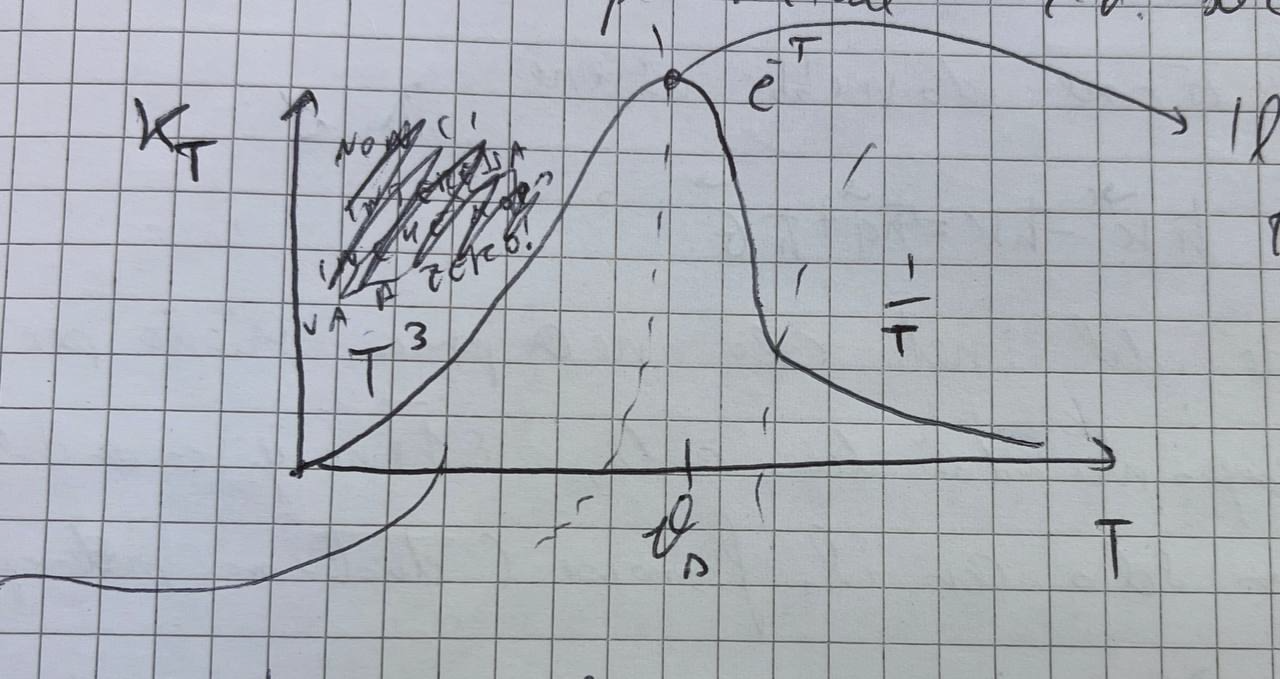
\includegraphics[width=0.5\linewidth]{img/asset2.png}
            \caption{Andamento di $k_{T, ph}$}
        \end{figure}
        Nella zona di sinistra rispetto al massimo le interazioni fononi-impurezze vincono rispetto a quelle fononi-fononi.\\
        Vediamo ora come i fononi influenzano la dipendenza dalla temperatura della conducibilità elettrica.\\
        Nel modello di Sommerfeld $\sigma = \displaystyle \frac{n e^{2}}{m_{e}}\tau $, la dipendenza da $T$ sta in $\tau$. Il $\tau$ è inversamente proporzionale alla frequenza di interazione elettrone-fonone:
        $$\tau \propto \frac{1}{W_{el-ph}}$$
        Se $\hbar \vec{k}', \ \hbar \vec{k}$ ed $h \vec{q}$ sono i momenti rispettivamente dell'elettrone post-urto, elettrone pre-urto e del fonone, allora vale:
        $$\hbar \vec{k} ' = \hbar \vec{k} +\hbar \vec{q}$$
        in pratica il fonone viene "assorbito" dall'elettrone. In realtà la relazione dovrebbe essere:
        $$\hbar \vec{k} ' - \hbar \vec{k} = \hbar \vec{q} + \hbar \vec{G}$$
        dove $\vec{G}$ è un vettore del reticolo reciproco. Questo vale perché l'elettrone comportandosi da onda interagisce anche con il reticolo e non solo con il fonone.\\
        Se $\vec{G} = 0$, vale $\hbar \vec{k} ' = \hbar \vec{k}+\hbar \vec{q}$ e si parla di \textbf{urti normali}, che sono i più rilevanti.
        Elidiamo $\hbar$:
        $$\vec{k}-\vec{k} = \vec{q} \implies E(k') - E(k) = E(q)$$
        Dunque:
        $$E(k') -E(k) =  \hbar \omega_{q}$$
        dove $\omega_{q}$ è la pulsazione associata al momento $\vec{q}$.
        L'energia fononica $\hbar \omega_{q}$ è trascurabile rispetto ad $E(k)$, che è nell'ordine della $E_{F} >> \hbar \omega_{q}$ anche nel caso in cui $\omega_{q} \sim \omega_{D}$.\\
        Allora:
        $$E(k') = \frac{\hbar ^{2} k'^{2}}{2m_{e}} = E(k) = \frac{\hbar ^{2}k^{2}}{2m_{e}} \implies |k'| = |k|$$
        Per i momenti questa cosa \textbf{non vale} perché a frequenze ragionevole abbiamo già detto che $|\vec{q}| \sim 1 \textrm{\si{\angstrom}} ^{-1}$.
        Riassumendo:
        $$\begin{cases}
            \vec{k'}-\vec{k} = \vec{q} \\
            k \simeq k' \simeq k_{F}
        \end{cases}$$
        Allora $\vec{k'}$ è un vettore di modulo praticamente par a $\vec{k}$, ma orientato in tutt'altro modo:
        \begin{figure}[h!]
            \centering
            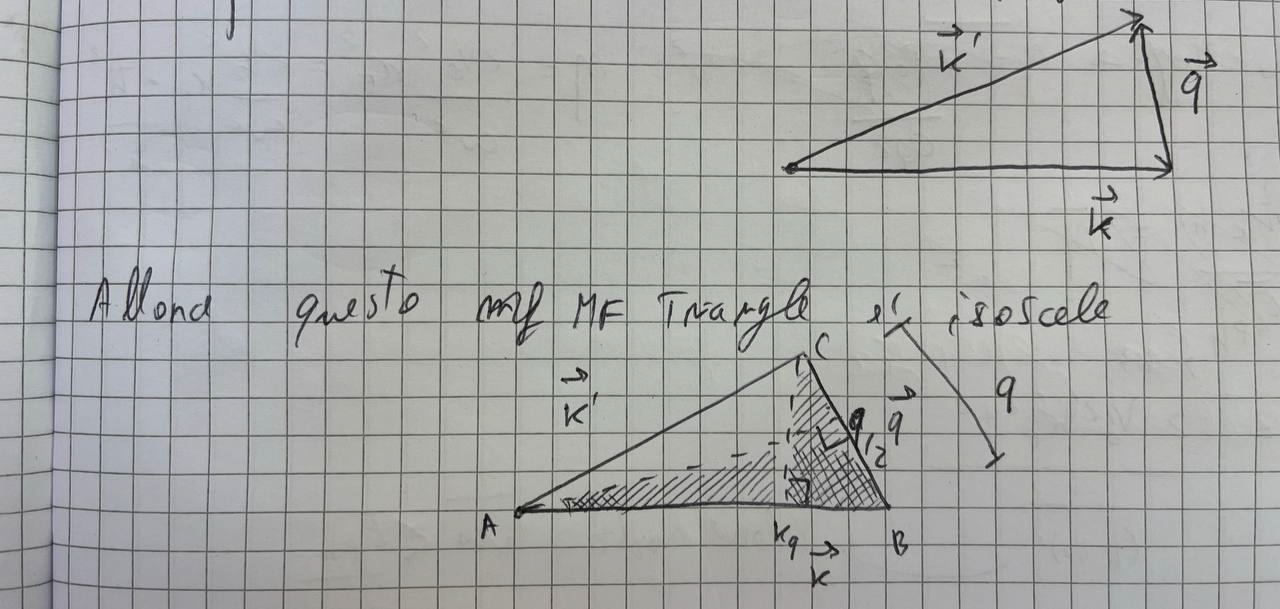
\includegraphics[width=0.85\linewidth]{img/pippo.png}
            \caption{Il triangolo di vettori è isoscele}
        \end{figure}
        La bisettrice che va da $A$ a $q/2$ è sia altezza che mediana del triangolo. I due triangoli ombreggiati (che si sovrappongono) sono \textbf\textbf{simili}, ergo si può scrivere:
        $$\frac{k_{q}}{q} = \frac{q/2}{k_{F}} \implies k_{q} = \frac{q^{2}}{k_{F}} \implies \frac{k_{q}}{k_{F}} = \frac{q^{2}}{2k_{F} ^{2}}$$
        e questo $\displaystyle \frac{k_{q}}{k_{F}}$ è, in un certo senso, l'entità con il quale l'interazione con i fononi disturba il moto degli elettroni, che può essere vista come "l'efficienza dell'urto", cioè quanti urti ci vogliono mediamente per annullare $\vec{k}$ nella direzione del suo moto.\\
        Definiamo anche il suo inverso:
        $$\eta = \frac{k_{F}}{k_{q}} = \frac{2k_{F} ^{2}}{q^{2}}$$
        Poiché $\omega = v_{0}q$ il valore medio di $\eta$ è:
        $$\eta = \frac{2v_{0} ^{2}}{\omega ^{2}}k_{F} ^{2} = \frac{\hbar ^{2}}{\hbar ^{2}} \cdot \frac{2v_{0} ^{2}}{\omega ^{2}}k_{F} ^{2} =  \frac{2v_{0} ^{2}k_{F} \hbar ^{2}}{\bar{(\hbar \omega)^{2}}}$$
        La quantità $\bar{(\hbar \omega)}^{2} = E_{ph}/n_{ph}$ e dunque:
        $$\tau \propto l_{el} \propto \frac{\bar{\eta}}{W_{el-ph}} \propto (\frac{n_{ph} ^{2}}{E_{ph}}) \cdot \frac{1}{n_{ph}}$$
        perché $\bar{n}_{ph}$ quantifica quanti urti servono per arrestare l'elettrone. In definitiva risulta:
        $$\sigma \propto \tau \propto (\frac{n_{ph}}{E_{ph}})^{2} \frac{1}{n_{ph}}$$
        Per $T>> \vartheta_{D}$ la dipendenza è del tipo $\displaystyle \frac{1}{T}$, mentre per $T<< \vartheta_{D}$ si ha una dipendenza del tipo $$\displaystyle \frac{1}{T^{5}}$$, perché $E_{ph}$ va come $\displaystyle \frac{1}{T^{4}}$ e $n_{ph}$ come $\displaystyle \frac{1}{T^{3}}$.\\
        La resistività da imputare ai fononi è ricavabile dalla formula di Bloch-Gru{\"u}neisen:
        $$\rho_{ph} (T) = \rho_{0} (\frac{T}{\vartheta_{D}}) ^{5} \int_{0} ^{\vartheta_{D}/T} \frac{t^{5}}{(e^{t}-1)(1-e^{-t})}$$
\chapter{Bande di Energia ed elettroni in un potenziale periodico}
    \section{Bande di energia}
        \paragraph{} In un atomo isolato ci sono vari livelli energetici:
            \begin{figure}[h!]
                \centering
                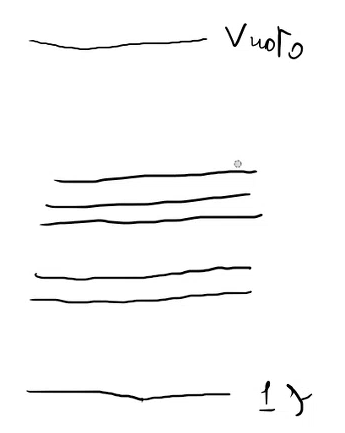
\includegraphics[width=0.35\linewidth]{img/chapSeiLivelliElettrone.png}
                \label{livelliEnergiaAtomoSingolo}
            \end{figure}
        \newpage
        \paragraph{} Ci si chiede allora cosa succede quando si considerando più atomi identici. Partiamo dal caso di due atomi identici, beneficiando del fatto che lo stesso concetto può essere esteso ad un insieme potenzialmente enorme di N atomi.

        Come sappiamo, tali livelli sono discreti e sono gli unici (potenzialmente infiniti) valori di energia che possono assumere gli elettroni dell'atomo. Graficando la relazione fra i livelli di energia $E$ e le distanze fra i nuclei dei due atomi $r$, è ragionevole dire che quando questi sono lontani i livelli di energia sono gli stessi dell'atomo isolato. Quando i due atomi iniziano ad avvicinarsi, cioè al diminuire di $r$, le funzioni d'onda associate al comportamento degli elettroni dei due atomi iniziano a sovrapporsi.
        \newline
        Consideriamo per esempio il valore dell'energia associato al livello $1s$. Quando $r$ diminuisce, l'autovalore di energia associato alla funzione d'onda che descrive quel livello energetico si splitta in due sottolivelli energetici, $1s'$ ed $1s''$, dunque ci sono quattro stati (ricordiamo che l'$1s$ ha due slot possibili per gli elettroni).\\
        \begin{figure}[h!]
            \centering
            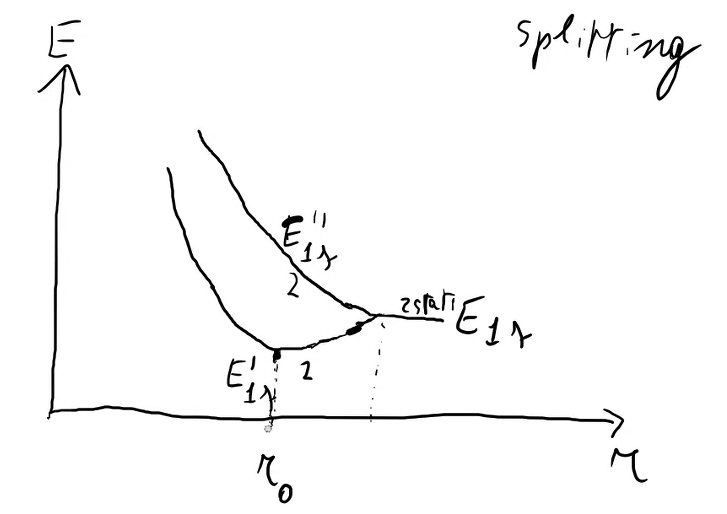
\includegraphics[width=0.5\linewidth]{img/Splitting2.png}
            \label{fig:splitting}
        \end{figure}

        \paragraph{}
            Come sappiamo ogni livello può ospitare al massimo $2(2l+1)$ elettroni, dunque nel caso generico con $N$ atomi ci saranno $2N(2l+1)$ possibili stati diversi, che nel caso dell'orbitale $1s$ ($l=0)$ corrisponde a $2N$. Graficamente, questo corrisponde all'infittirsi delle curve "originate" dallo split dello stato preso in considerazione, che possiamo considerare praticamente continua:
            \begin{figure}[h!]
                \centering
                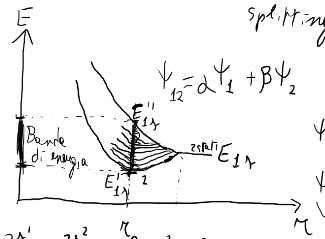
\includegraphics[width=0.5\linewidth]{img/Splitting3.png}
                \label{fig:Splitting3}
            \end{figure}
            \paragraph{} Con la rappresentazione a bande è facile distinguere conduttori ed isolanti: i primi avranno una delle bande semipiene, mentre i secondi avranno solo bande piene o vuote. Le bande sono formalmente infinite, perché sono infiniti il numero di livelli di energia, ma ovviamente ci si ferma a quelle bande associati a valori di energia che si possono ragionevolmente raggiungere.
    \section{Teorema di Bloch}
        \paragraph{} Nel modello ad elettroni liberi la funzione potenziale $U(r)$ che tiene conto dell'interazione degli elettroni con altri oggetti (il nucleo) è assunta nulla. Qui non possiamo fare tale assunzione e dunque l'equazione di Schroedinger che descrive più correttamente il comportamento degli elettroni contiene un contributo $U(r)$ che è un potenziale periodico di passo reticolare $\vec{R}=n_{1}\vec{a}_{1}+n_{2}\vec{a}_{2}+n_{3}\vec{a}_{3}$.
        $$\hat{H}\Psi = E \Psi \iff - \frac{h^{2}}{2m_{e}} \nabla \Psi + U(\vec{r}) = E \Psi$$

        \paragraph{Il teorema di Bloch} afferma, nel caso in cui il termine $U(\vec{r})$ che compare nell'espressione della funzione d'onda sia periodico di $\vec{R}$, allora l'autofunzione corrispondente all'autovalore $n$ si può scrivere come:
        $$\Psi_{\vec{k}}(\vec{r}) = e^{i\vec{k}\cdot \vec{r}} u(\vec{r})$$
        dove $u(\vec{r})$ è una funzione periodica di $\vec{R}$. Per un autovalore $n$ ci potrebbero essere varie $\Psi_{k}$ che sono soluzione. \newline
        Una proprietà interessante che discende dal teorema di Bloch è la periodicità delle soluzioni nello spazio dei momenti, cioè:
        $$\Psi_{\vec{k}+\vec{G}} = e^{i\vec{G} \cdot \vec{r})}e^{i\vec{k} \cdot \vec{r})}u(r) = e^{i\vec{G} \cdot \vec{r})}\Psi_{\vec{k}}$$. Ora poiché il prodotto $\vec{G} \cdot \vec{R} = 2 \pi n$, con $n \in \mathbb{N}$ (vedi lezioni sui reticoli reciproci), la quantità $e^{i\vec{2 \pi n}} = 1$ e allora:
        $$\Psi_{\vec{k}+\vec{G}}(\vec{r}+\vec{R}) = e^{i\vec{G} \cdot \vec{r}}e^{i\vec{G} \cdot \vec{R}} \Psi_{\vec{k}} = e^{i\vec{G} \cdot \vec{r}}\Psi_{k} = \Psi_{\vec{k}+\vec{G}}(\vec{r})$$.
        Questo significa che anche gli autovalori delle energie sono periodici nello spazio dei momenti:
        $E(\vec{k}) = E(\vec{k}+\vec{G})$
        e dunque grazie al teorema di Bloch si possono ricavare gli autovalori in una cella elementare per conoscere tutti gli altri autovalori associati ad autofunzioni relative ad un generico vettore $\vec{k}+\vec{G}$ dello spazio dei momenti. \newline
        La cella elementare che viene scelta è quella di \textbf{Brillouin} (vedi lezione sui reticoli reciproci).


        \section{Elettroni con debole potenziale periodico}
            \paragraph{}
                Consideriamo un "debole" potenziale di interazione con gli ioni. Partiamo da Schroedinger in una dimensione:
                $$\frac{-\hbar}{2m_{e}} \frac{\partial  ^{2} \Psi (x)}{\partial x^{2}} + U(x)\Psi(x) = E\Psi (x)$$

                con $U(x) = U(x+na)$

            \paragraph{}
                Se $U(x)$ è periodica, si può sviluppare in serie di Fourier:
                $$U(x) = \sum_{n} U_{n}e^{-i\frac{2\pi}{a}nx}$$
                Anche la funzione di Bloch è periodica e può essere sviluppata:
                $$Y(x) = e^{ikx}u(x) = e^{ikx} \sum_{n} c_{n}e^{-i \frac{2\pi}{a}nx}$$

                Facciamo la derivata seconda di $\Psi(x)$:
                $$\frac{\partial ^{2} \Psi (x)}{\partial x^{2}} = -e^{ikx} \sum_{n} c_{n}e^{-i\frac{2\pi}{a}nx} (k- \frac{2\pi}{a}n)^{2}$$

                Dunque:
                $$e^{ikx} [\sum_{n} \frac{\hbar ^{2}}{2m_{e}}(k-\frac{2\pi}{a}n)^{2}c_{n}\exp{(-i\frac{2\pi}{a}nx)} + \sum_{n'} \sum_{n''} U_{n''}c_{n'} \exp{(-i\frac{2\pi}{a}(n''+n')x)}]$$
                che deve essere uguale a:
                $$e^{ikx}\sum_{n} Ec_{n} \exp{(-i\frac{2\pi}{a}nx)}$$

                Semplificando $e^{ikx}$ ambo i lati e ponendo $n=n''+n' \implies n''=n-n'$, perché tanto gli indici variano in $[-\infty, +\infty]$, risulta, riorganizzando l'espressione:
                $$\sum_{n} [E - \frac{\hbar ^{2}}{2m_{e}}(k - \frac{2\pi }{a}n)^{2}]c_{n}\exp{(-i\frac{2\pi}{a}nx)} = \sum_{n'}U_{n-n'}c_{n'}\exp{(-i\frac{2\pi}{a}nx)} $$

                Uguagliando i coefficienti delle sommaotorie (le autofunzioni in $n$ so le stesse ambo lati):
                $$[E - \frac{\hbar ^{2}}{2m_{e}}(k - \frac{2\pi }{a}n)^{2}]c_{n}= \sum_{n'}U_{n-n'}c_{n'} $$

                Poniamoci nel caso limite dove: 
                $$U(x) = 0\quad \forall x \implies U_{n} \quad \forall n$$
                dunque:
                $$[E - \frac{h^{2}}{2m_{e}} (k-\frac{2\pi}{a} n )^{2}]c_{n} = 0$$
                Le alternative sono due: o $c_{n} = 0 \quad \forall n$, ed è impossibile perché sennò  la $\Psi(x)$ sarebbe identicamente nulla, oppure (soluzione):
                $$E_{k,n} \frac{\hbar^{2}}{2m_{e}} (k- \frac{2\pi}{a}n)^{2} = 0$$

                Per $n=0 \implies E_{0}(k) = \displaystyle \frac{\hbar ^{2}k^{2}}{2m_{e}}$, energia dell'elettrone libero. Per $n>0$ la parabole in funzione di $k$ trasla di centro $\frac{2\pi}{a}$.
                \begin{figure}[h!]
                    \centering
                    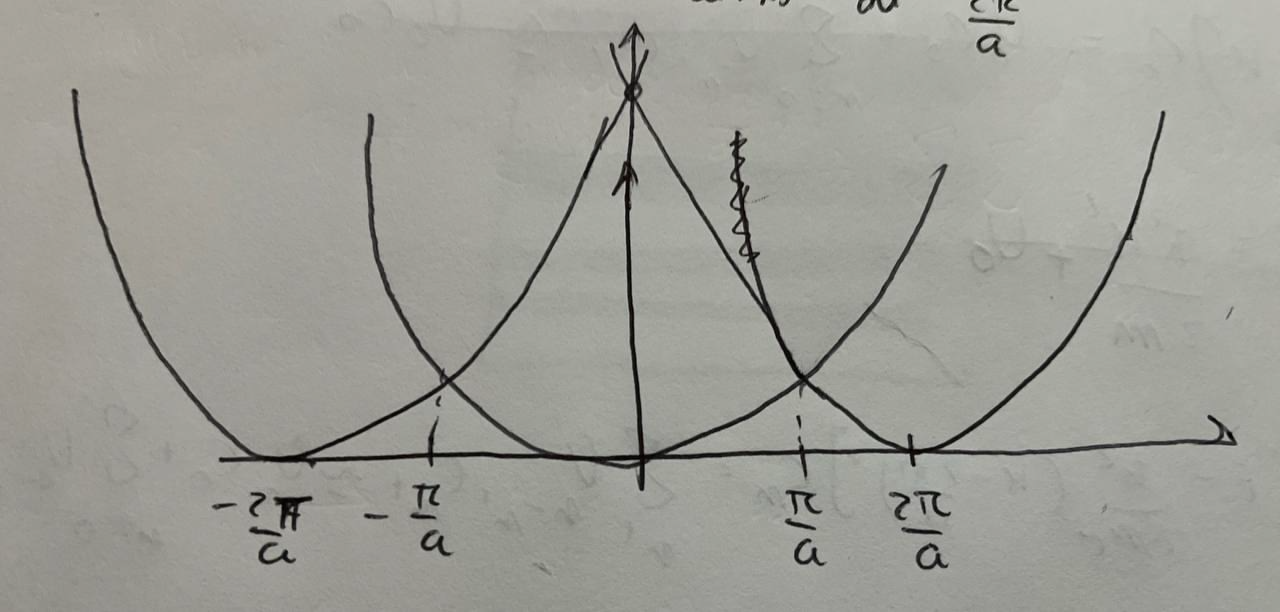
\includegraphics[width=0.5\linewidth]{img/paraboloneLez20.png}
                    \caption{Plot di E(k) variando n}
                \end{figure}
                L'intersezione di ste parabola si ripetono per $\displaystyle \frac{2 \pi}{a}$, dunque possiamo prendere come riferimento la prima zona di Brillouin $[-\frac{\pi}{a}; \frac{\pi}{a}]$, poi il comportamento si ripeterà in modo periodico.

                \paragraph{}
                    Ipotizziamo ora che $U(x)>0$ ma "debole", cioè abbastanza piccolo per il quale la situazione mostrata in figura 4.1 non cambi troppo. In questo caso $c_{n} \neq 0$ e dunque risulta:
                    $$[E - \frac{\hbar ^{2}}{2m_{e}}(k - \frac{2\pi }{a}n)^{2}]c_{n}= \sum_{n'}U_{n-n'}c_{n'} $$

                    da cui possiamo scrivere:
                    $$[E - \frac{\hbar ^{2}}{2m_{e}}(k - \frac{2\pi }{a}n)^{2}]c_{n}= U_{n}c_{0}\sum_{n' \neq 0}U_{n-n'}c_{n'} $$
                    allora per $n=0$ $E = \displaystyle \frac{\hbar ^{2}}{2m_{e}}k^{2} + \frac{1}{c_{0}} \sum_{n'} U_{-n'}c_{n'}$
                    con:
                    $$c_{n} \frac{\sum_{n'}U_{n-n'}c_{n'}}{E - \frac{\hbar ^{2}}{2m_{e}}(k - \frac{2\pi }{a}n)^{2}} \simeq \frac{U_{n}c_{0}}{E - \frac{\hbar ^{2}}{2m_{e}}(k - \frac{2\pi }{a}n)^{2}}$$
                    L'ultimo passaggio è giustificato se il potenziale è piccolo. Allora:
                    $$E = \frac{\hbar ^{2}}{2m_{e}}k^{2} + \sum_{n'} \frac{|U_{n'}|^{2}}{E - \frac{\hbar ^{2}}{2m_{e}}(k - \frac{2\pi }{a}n)^{2}}$$
                    che è un equazione implicita in $E$.
                    Rispetto alla funzione per $U(x)$ nullo (tratteggiata in figura), per potenziali deboli varia leggermente e ha una discontinuità ogni $\pi/a$, perché il denominatore del secondo pezzo del secondo membro si annulla. Allora si identificano le \textbf{bande di energia} come gli spazi fra un gap e un altro, mente le \textbf{bande proibite} sono i gap stessi. Notiamo che all'aumentare di $n$ aumentano le larghezze delle bande, che ai primi valori di $n$ sono praticamente gruppi di valori discreti.
                    \begin{figure}[h!]
                        \centering
                        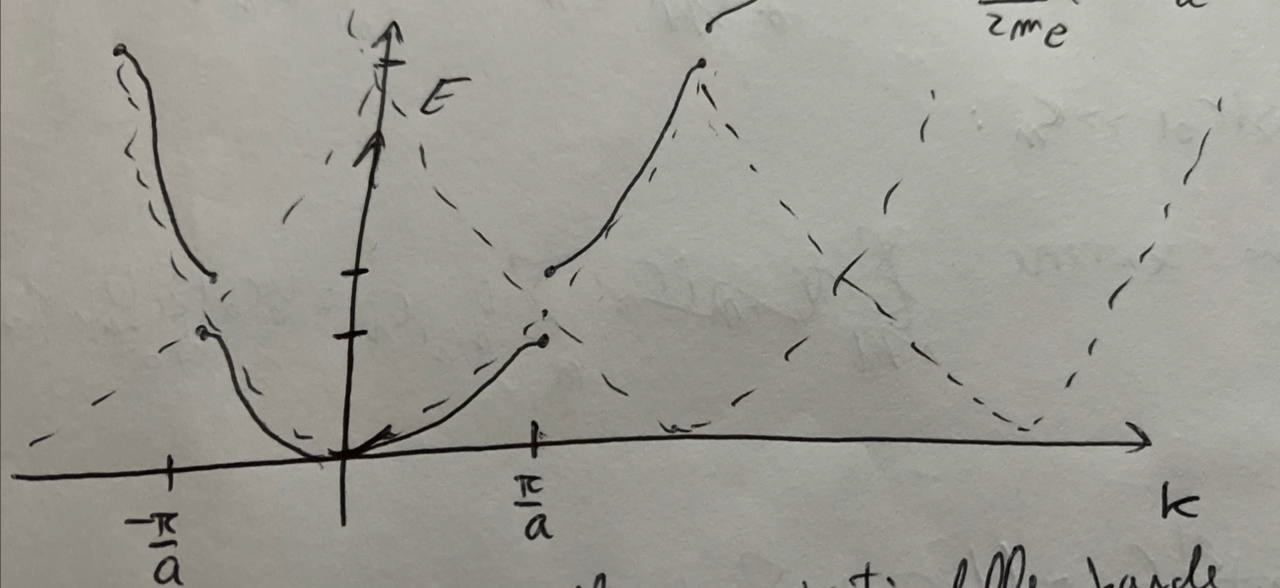
\includegraphics[width=0.5\linewidth]{img/crostiniLez20.png}
                        \caption{Plot di E(k) per weak potential}
                    \end{figure}
                    
            \section{Lacune}
                Nota: qui mi sono confuso e per una dimensione ho messo il segno di vettore per $k, v$ e tutto il resto, pensando alle tre dimensioni. Ignorate se leggete e pensate semplicemente al modulo della singola componente monodimensionale, in tre dimensioni si generalizza considerando i gradienti e le derivate miste.
                \paragraph{}
                    Gli ingegneri elettronici sono abituati a rappresentare le bande di energia nel grafico monodimensionale di valori di $E$, dove le bande rappresentano i valori ammessi, mentre in questo caso viene evidenziata la dipendenza da $k$. Quello che lega i due grafici essenzialmente è che se esiste qualche valore di $k$ per il quale qualche elettrone può assumere un determinato livello di energia, allora esiste un livello energetico corrispondente. Infittendo questa cosa si generano le bande:
                    \begin{figure}[h!]
                        \centering
                        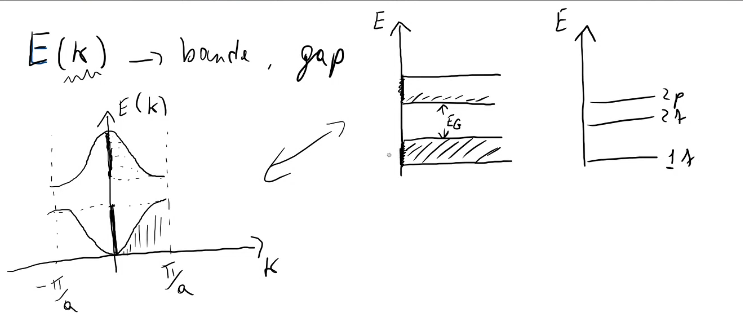
\includegraphics[width=0.75\linewidth]{img/Lez21pt1.png}
                        \caption{A sx grafico delle energie in funzione di $k$, a dx classica rappresentazione a bande}
                        \label{fig:rappresentazioneABande}
                    \end{figure}\\
                    La funzione rappresentata nel grafico $E = E(k)$ è detta \textbf{funzione di dispersione della banda} e tipicamente ogni solido ne ha una differente.
                    Scriviamo la velocità di gruppo dell'onda associata al generico elettrone del cristallo in funzione di $dE(k)/dk$, sfruttando le relazioni di De Broglie:
                    $$\vec{v} = \frac{d \omega}{dt} = \frac{1}{\hbar} \frac{d \hbar \omega}{dt} = \frac{dE(k)}{dt}$$
                    La funzione di dispersione della banda è simmetrica rispetto all'asse delle ordinate, dunque la derivata calcolata in $k$ è opposta a quella calcolata in $-k$, ragion per la quale sommando tutte le velocità di gruppo degli elettroni, quella netta è nulla, perché i termini si annullano a coppie (statisticamente per ogni $k$ c'è uno stato $-k$ occupato). Macroscopicamente questa cosa corrisponde all'assenza di corrente elettrica.\\ \\
                    Derivando rispetto a $t$:
                    $$\frac{d\vec{v}}{dt} = \frac{1}{\hbar} \frac{d ^{2} E}{dk^{2}} \frac{dk}{dt} = \frac{1}{\hbar} \frac{d^{2}E(k)}{dk^{2}} \frac{d\hbar k}{dt}$$
                    da cui:
                    $$\frac{d(\hbar k)}{dt} = (\frac{1}{\hbar ^{2}} \frac{d^{2}E(k)}{dk^{2}}) ^{-1} \frac{d\vec{v}}{dt}$$
                    Questa relazione ci da conferma che $\hbar k$ in questo caso non è la quantità di moto dell'elettrone. Infatti la derivata rispetto al tempo di $\vec{p} = m_{e}\vec{v}$ dovrebbe essere proporzionale alla massa dell'elettrone, cosa che non accade nella relazione scritta sopra. Chiamiamo la quantità che moltiplica $d\vec{v}/dt$ \textbf{massa efficace}, indicata con $m^{*}$:
                    $$\frac{d (\hbar k)}{dt} = m^{*} \frac{d\vec{v}}{dt}$$
                    In generale $m^{*} \neq m_{e}$ e non è detto che sia costante, dipende dalla funzione di dispersione della banda.

                    \paragraph{}
                        Sviluppiamo con Taylor la funzione $E(K)$ in corrispondenza di $k_{0}$, punto per il quale assume minimo (ricordiamo che la funzione è periodica quindi analoghe considerazioni per ogni zona di Brillouin):
                        $$E(k) = E(k_{0}) + \frac{1}{2} \frac{d^{2}E(k}{dk^{2}}|_{k=0} (k-k_{0}) $$
                        dove il termine di ordine uno è nullo perché si tratta di un minimo.
                        Riscriviamola per tirare fuori l'espressione della massa efficace:
                        $$E(k) \simeq E(k_{0}) + \frac{1}{2}  \frac{\hbar}{\hbar}\frac{d^{2}E(k}{dk^{2}}|_{k=0} (k-k_{0})^{2} = E(k_{0}) + \frac{\hbar ^{2}}{2m^{*}}(k-k_{0})^{2} $$
                        dove $m^{*}$ è valutata in $k=k_{0}$. In pratica, nei pressi del minimo di banda si può "riciclare" il modello di Sommerfeld per elettroni liberi, a patto di considerare la massa efficace al posto di quella elettronica per tener conto del potenziale cristallo (il quale, ovviamente, rende l'elettrone "non libero").Per come abbiamo disegnato il grafico noi, la derivata seconda è positiva e dunque anche la massa efficace (torneremo dopo sulle considerazioni per il punto di massimo, dove la concavità è negativa).
                        Considerazione estendibile anche se non si è al limite di banda: se si considera una forza esterna agente sugli elettroni, questa vale:
                        $$\vec{F}_{ext} = m^{*} \frac{d \vec{v}}{dt} = \frac{d (\hbar \vec{k})}{dt}$$
                        Apparentemente c'è contraddizione in ciò che abbiamo appena scritto, perché abbiamo ribadito che la quantità di moto dell'elettrone \textit{non} è $\hbar k$. La forza $F_{ext}$ però non è l'unica forza che agisce sull'elettrone, perché bisogna considerare gli effetti cristallini e tutto il resto, quindi ciò che abbiamo scritto rimane lecito.\\
                        Dunque dalla forza esterna da ascrivere al campo elettrico applicato all'esterno si ricava l'espressione di $\vec{k}(t)$:
                        $$\vec{F}_{ext} = \hbar \frac{d\vec{k}}{dt} \implies -\frac{e\vec{E}_{0}}{\hbar} = \frac{d \vec{k}}{dt} \implies \vec{k}(t) = \vec{k}_{0}- \frac{e \vec{E_{0}}}{\hbar} t$$
                        Prima dell'accensione del campo elettrico (\textbf{costante}), plottando gli stati (cerchi pieni quelli occupati, vuoti quelli liberi) sulla alla funzione di dispersione:
                        \begin{figure}[h!]
                            \centering
                            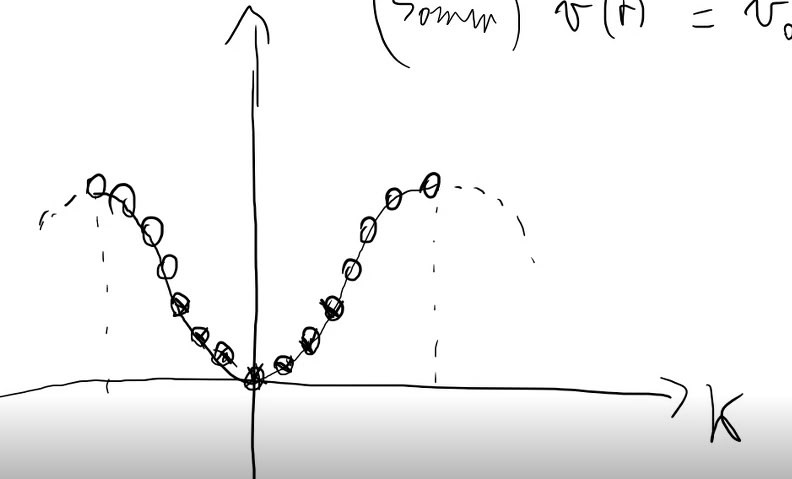
\includegraphics[width=0.5\linewidth]{img/plotLez21.png}
                        \end{figure}
                        All'accensione $k$ deve aumentare linearmente di $-e \frac{\vec{E_{0}}}{\hbar}$, di fatto shiftando a destra nel grafico (cerchi verdi nuovi stati pieni, il resto vuoti):
                        \begin{figure}[h!]
                            \centering
                            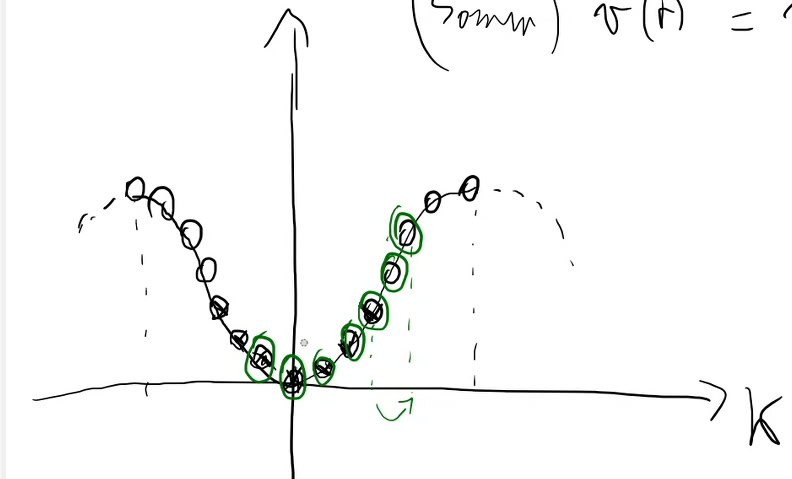
\includegraphics[width=0.5\linewidth]{img/plot2lez21.png}
                        \end{figure}
                        In quest'ultima situazione non c'è più velocità media nulla, perché non c'è simmetria di "occupazione degli stati" rispetto alle ordinate. Insorge allora una corrente elettrica. Andando avanti nel tempo c'è ancora shift a destra, ma per periodicità se un elettrone occupa uno stato al di fuori della prima zona di Brillouin $[-\pi/2, \pi/2]$, un altro arriva dalla zona di sinistra:
                        \begin{figure}[h!]
                            \centering
                            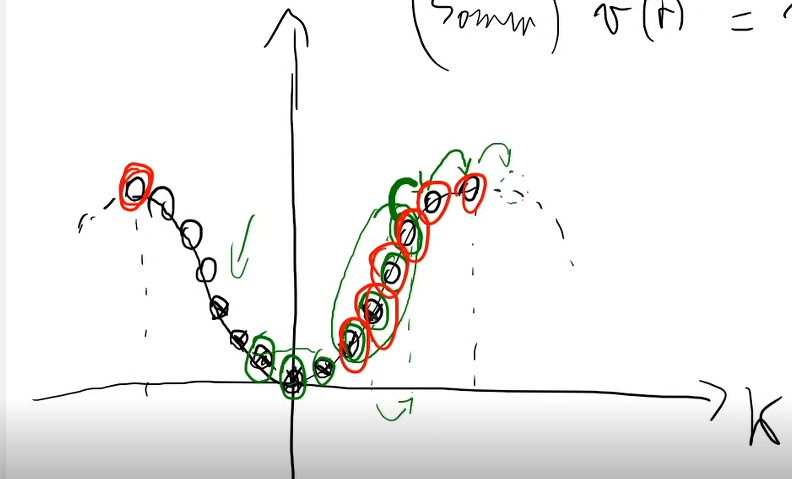
\includegraphics[width=0.5\linewidth]{img/plot3lez21.png}
                        \end{figure}
                        Non abbiamo allora il problema della velocità media divergente. 
                        Ad una certa si arriva a questa situazione qua:
                        \begin{figure}[h!]
                            \centering
                            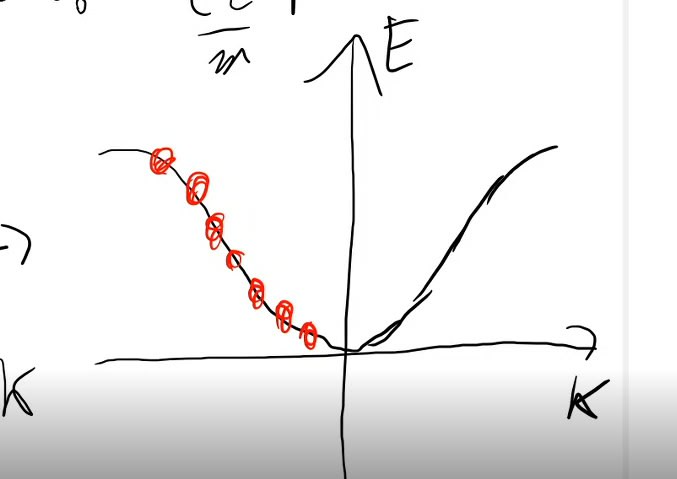
\includegraphics[width=0.5\linewidth]{img/plot4lez21.png}
                        \end{figure}
                        dove la velocità media ha valori negativi. Da qui l'assurdo: con un campo elettrico costante (dovrebbe venir) generata una corrente alternata. Deve allora esistere un meccanismo di saturazione di $\vec{k}$. Posto $\Delta \vec{k} = \vec{k} - \vec{k}_{0}$ e considerando un termine corretto di tipo viscoso:
                        $$\frac{d (\hbar \Delta \vec{k}(t))}{dt} = -e \vec{E}_{0} - \frac{\hbar \Delta \vec{k}(t)}{\tau}$$
                        che satura al valore:
                        $$\Delta \vec{k}(t)_{sat} = -e\frac{\vec{E}_{0}\tau}{\hbar} $$
                        Da queste considerazioni si capisce perché gli ioni non sono da ascrivere al comportamento di saturazione di $\vec{k}(t)$, come uno potrebbe naturalmente pensare che accada. Avevamo già anticipato che gli elettroni non sbattono veramente contro gli ioni del reticolo, il cui contributo è inglobato nella massa efficace $m^{*}$. In altre parole, la perfetta periodicità della funzione di dispersione a bande \textbf{non c'entra} con il meccanismo di saturazione, che è da attribuire ad altra causa.
                        Ciò che rompe la periodicità e da vita al fenomeno della resistività elettrica sono le impurezze del cristallo e il fatto che gli atomi non stanno fermi nelle loro posizioni d'equilibrio per $T \geq 0$.

                    \paragraph{}
                        Consideriamo ora l'espressione della densità di corrente. Tenendo conto che, approssimativamente, possiamo scrivere il numero di portatori per unità di volume $n$ come $\frac{N}{V}$, con $N$ numero di portatori, esprimendo la velocità media (velocità di drift) come sommatoria uniformemente pesata:
                        $$\vec{J} = -ne\vec{v}_{d} = -e \frac{N}{V} \frac{1}{N} \sum_{i_{occ}} ^{N_{occ}} \vec{v_{i}} = -e \sum_{i_{occ}} ^{N_{occ}} \vec{v}_{i}$$
                        dove si è tenuto conto che la velocità media va valutata solo su gli indici e sul numero degli stati occupati. Ora tenendo conto che la velocità media totale valutata su \textit{tutti} gli stati è nulla per simmetria della funzione di dispersione, ricaviamo:
                        $$\sum_{i} ^{N} \vec{v}_{i} = \sum_{i_{occ}} ^{N_{occ}} \vec{v}_{i_{occ}}+\sum_{i_{vuoti}} ^{N_{vuoti}} \vec{v}_{i_{vuoti}} = 0$$
                        Alché:
                        $$\vec{J} = e \sum_{i_{vuoti}} ^{N_{vuoti}} \vec{v}_{i}$$
                        Che significa? Che la densità di corrente si può vedere come prodotto fra la velocità media degli stati occupati per la carica dell'elettrone \textit{oppure} come il prodotto fra \textbf{cariche positive} (lacune) per la velocità media degli stati vuoti.
                        Per capire meglio questa cosa, mettendosi nel grafico $E(k)$ (non c'è disegnata l'asse delle ascisse), l'elettrone (in nero) per fare il salto di stato e sostituirsi quindi ad uno stato vuoto (una lacuna) spende un certo tipo di energia.
                        \begin{figure}[h!]
                            \centering
                            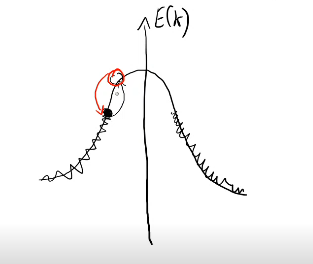
\includegraphics[width=0.5\linewidth]{img/radio1.png}
                        \end{figure}
                        \newpage
                        Conversely, we should consider gaps' energy along the opposite direction of $E(k)$, as shown in figure, for they are gaining energy:
                        \begin{figure}[h!]
                            \centering
                            \includegraphics[width=0.5\linewidth]{img/radio2.png}
                        \end{figure}
                        The maximum energy level an electron can reach is $E_{M}$. Thus, we can define $E'_{p}(k)$, the energy of the gap occupying the slot $k$, as:
                        $$E'_{p}(k) = E_{M} - E_{n}(k)$$
                        where $E'_{n}(k)$ is the energy of the electron occupying the slot $k$.
                        Therefore the minimum energy value for gaps is the maximum value for electrons and vice-versa.
                        From effective mass definition, we obtain:
                        $$m_{p} ^{* \ -1} = \frac{1}{\hbar ^{2}} \frac{d^{2}E'_{p}(k)}{d ^{2}k} = - \frac{1}{\hbar ^{2}} \frac{d^{2}E_{n}(k)}{d ^{2}k} = -m_{n} ^{* \ -1}$$
                        To be clear, $m^{*} _{p}$ is the effective mass that one would obtain calculating the effective mass for electrons referring to the band-dispersion function $E'_{p}(k)$. But as we are considering the opposite axis $E'(x)$  to describe gaps' energy values, it's still positive even if the second derivative is negative.\\
                        In three dimension one can derive:
                        $$\vec{v}_{p} = \vec{\nabla}_{k} \vec{E}_{p}(k) = - \vec{\nabla}_{k} \vec{E}_{n} (k) = -\vec{v}_{n}$$
                        So a gap is a particle whose effective mass and average velocity are opposite to that of the electron. The Fermi-Dirac function tells us the probability for the state at energy level $E$ to be occupied, therefore the probability for that state to be occupied by a gap (namely not occupied) is:
                        $$P(gap(E)) = 1- f(E)$$
                        We shall now translate what we've just said for a tridimensional space. First of all, the effective mass is a tensor $\mathbb{M}$ whose components $m_{ij} ^{*}$ are defined as such:
                        $$m_{ij} ^{*} = \frac{1}{\hbar ^{2}} (\frac{\partial^{2}E_{p}(k)}{\partial k_{j}\partial k_{i}}) ^{-1}$$
                        for one should consider the mixed derivatives. Therefore the outer force $\vec{F}$ can be written as:
                        $$\vec{F} = \mathbb{M} \vec{a}$$
                        namely the tensor product between $\mathbb{M}$ and $\vec{a}$.
                        For the energies, similarly:
                        $$E(\vec{k}) = \frac{\hbar ^{2}}{2m_{e}} = [(k_{x} - \frac{2 \pi}{a}h)^{2}+(k_{y} - \frac{2 \pi}{a}k)^{2}+(k_{z} - \frac{2 \pi}{a}l)^{2}]$$
                        Please notice that $k$ is Miller index and not a component of $\vec{k}$.
                        The concept of DoS can be generalized as well, considering a surface living $S$ in the space of $k$, which depends on a fixed $E =E(\vec{k})$:
                        $$N(E) = \frac{1}{4 \pi^{3}} \int_{S(E)} \frac{dS}{|\vec{\nabla}_{k}E(\vec{k})|}$$
                       

            \section{Microscopi elettronici SEM e TEM}
                SEM sta per "Scanning Electronic Microscope" mentre TEM per "Transmission Electronic Microscope". 
                Per i microscopi SEM le energie che si utilizzano vanno dalle frazioni di keV fino 
                alle decine di keV. I SEM funzionano in riflessione e difficilmente raggiungono risoluzione atomica, mentre 
                i TEM hanno risoluzione molto più alta.
                \subsection*{Il SEM}
                        Il fascio elettronico viene guidato da campi elettrici variabili nel tempo 
                        ad eseguire una scansione superficiale rettangolare, linea per linea. Si tratta
                        con energie che vanno da frazioni a qualche decina di keV. Quando il fascio elettronico
                        incide sulla superficie da scansionare, hanno luogo due fenomeni. La prima è la riflessione 
                        all'indietro degli elettroni, fenomeno di \textit{back scattering}, il quale avviene in modo elastico.
                        La seconda è l'emissione di raggi X dovuti all'eccitazione degli elettroni ai livelli interni, che emettono 
                        tali raggi una volta diseccitati. Quelli che danno l'immagine caratteristica del SEM sono gli \textbf{elettroni secondari},
                        cioè quegli elettroni prelevati dai livelli energetici superiori che sono meno legati all'atomo. Gli \textbf{elettroni primari},
                        che vengono estratti ad energie più alte (corrispondenti al livello di penetrazione del fascio, dal nanometro a qualche micron) sono 
                        ovviamente più difficili da estrarre e vengono ricatturati nella nube elettronica mentre risalgono in superficie.
                        In sintesi, i SEM danno immagini basate sugli elettroni retrodiffusi, più sensibili alle caratteristiche interne del campione. Inoltre,
                        forniscono un contrasto differente nel caso di larghe zona costituite da elementi dfferenti, permettendo quindi
                        \textbf{un'identificazione qualitativa della presenza di specie chimiche differenti sul campione}. Questa cosa è permessa perché
                        lo scattering all'indietro è maggiore per gli atomi più grandi.
                \subsection*{Il TEM}
                        Il TEM differisce dal SEM nel fatto che vengono raccolti gli elettroni trasmessi dal campione 
                        e non quelli riflessi all'indietro. Affinché ciò accade, occorre un campione molto sottile, cosicché gli 
                        elettroni non vengano catturati dalla nube elettronica. A fronte di ciò, è molto più complicato utilizzare un TEM
                        piuttosto che un SEM, con la ricompensa di una risoluzione maggiore. Per il TEM esistono apposite tecniche per il "taglio"
                        dei campioni solidi da misurare, che vengono disposti lungo griglie costituite da metalli o fibra di carbonio con 
                        spessori "sottili" nell'ordine dei 100$\mu$m. A differenza del SEM, nel TEM il fascio non viene inciso linea per linea ma
                        contemporaneamente su tutta la superficie e dunque non è necessario focalizzare il fascio con complicati sistemi di specchi e leve.
                        In conclusione, l'angolo di scattering  sarà mediamente maggiore per le specie atomiche più "grosse", potendo distinguere un materiale
                        da un altro.
\chapter{Semiconduttori}
    \section{Caratteristiche generali}
        Schematizziamo in maniera approssimativa il grafico di due bande nel piano $E(k), k$, dove $k$ è il momento cristallino ed $E(k)$ il livello di energia.
        \begin{figure}[h!]
            \centering
            \includegraphics[width=0.5\linewidth]{img/radio4.png}
        \end{figure}
        In basso c'è la banda di valenza, indicata con $B_{V}$ ed energia massima $E_{V}$, mentre in alto c'è la banda di conduzione, indicata con $B_{C}$ ed energia minima $E_{C}$. Va da sè che l'energia di gap è $E_{G} = E_{C} - E_{V}$.\\
        Per effetto dell'agitazione termica, capita che alcuni elettroni si portino dalla banda di valenza a quella di conduzione, facendo si che delle lacune si portino in banda di valenza. Ricordiamo che la massa efficace per gli elettroni è calcolata sul fondo della banda di conduzione, dove la concavità e positiva (e dunque pure la $m^{*}_{n}$. Per le lacune invece, la massa efficace viene calcolata sulla cima della banda di valenza, ove la pendenza è negativa, ragion per la quale $m^{*}_{p} = - m_{el}^{*}(E_{V})$, dove $m_{el}^{*}(E_{V})$ è la massa efficace calcolata su un elettrone che si trova nel medesimo livello di energia (il pedice "el" si distingue da "n" perché il secondo di solito fa riferimento agli elettroni valutati in banda di conduzione).\\
        Con l'ipotesi fatta nel capitolo precedente di poter sviluppare con Taylor l'espressione dei livelli di energia, associati ad elettroni e lacune di momento cristallino $k$, in prossimità rispettivamente del minimo della banda di conduzione e del massimo della banda di valenza, sono:
        $$E_{n}(k) = \frac{\hbar ^{2}}{2m_{e} ^{*}}(k-k_{0})^{2} \qquad E_{p}(k) = \frac{\hbar ^{2}}{2m_{p} ^{*}}(k-k_{0})^{2}$$
        Possiamo definire per entrambi anche una DoS simile a quella ricavata nel modello di Sommerfeld:
        $$N_{n}(E) = \gamma_{n}(E-E_{V})^{1/2} \qquad N_{p} = \gamma_{p}(E_{C}-E)^{1/2}$$
        Queste espressioni hanno perfettamente senso se si tiene conto che le lacune in $B_{V}$ possono avere al massimo energia $E_{C}$, mentre gli elettroni in $B_{C}$ al minimo energia $E_{C}$.
        Il parametro gamma è lo stesso di Sommerfeld, ma va sostituita la massa elettronica con quelle efficaci $m_{n} ^{*}$ ed $m_{p} ^{*}$.
    \section{Semiconduttori intrinseci}
        I semiconduttori intriseci sono quelli che hanno banda di valenza piena e banda di conduzione vuota. Per ogni elettrone che va in banda di conduzione, c'è una lacuna in banda di valenza, dunque se definiamo $n$ e $p$ come le densità rispettivamente di portatori in banda di conduzione (elettroni) e di valenza (lacune), otteniamo:
        $$n = p$$
        Per ricavare il valore di questi due parametri scriviamo l'espressione del numero di portatori per unità di volume:
        $$\rho_{n}(E) = N_{n}(E)f(E) \qquad \rho_{p}(E) = N_{p}(E)[1-f(E)]$$
        avendo fissato $T$ così che la funzione di Fermi-Dirac dipenda soltanto da $E$. Allora integriamo sui valori possibili delle energie assunte dai portatori nelle rispettive bande. Partiamo dagli elettroni
        $$n = \int_{E_{C}} ^{\infty} \rho_{n}(E)dE = \int_{E_{C}} ^{\infty} \gamma_{n}(E-E_{C})^{1/2}\frac{1}{\exp{(\frac{E-E_{F}}{k_{B}T}})-1}$$
        Sotto la ragionevole ipotesi $E-E_{F} >> k_{B}T$ risulta:
        $$\rho_{n}(E) \simeq    \gamma_{n} \int_{E_{C}} ^{\infty} (E-E_{C})^{1/2}\exp{(\frac{E_{C}-E_{F}}{k_{b}T})} = \frac{\sqrt{\pi}}{2} \gamma_{n}(k_{B}T)^{3/2}\exp{(\frac{-(E_{C}-E_{F})}{k_{B}T})} = 
        $$
        $$N_{C}(T)\exp{(\frac{-(E_{C}-E_{F})}{k_{B}T})}$$
        dove $N_{C}(T)=\frac{\sqrt{\pi}}{2} \gamma_{n}(k_{B}T)^{3/2}$.
        Sostituendo l'espressione di $\gamma_{n}$ in quella di $N_{C}(T)$ si ricava una delle risposte del quiz a crocette:
        $$N(C) = \displaystyle 2(\frac{2 \pi m_{n} ^{*}k_{B}T}{h^{2}})^{3/2}$$
        In modo analogo per $p$
        $$p = N_{V}(T)\exp{(\frac{-(E_{F}-E_{V})}{k_{B}T})}$$.
        dove $N_{V}(T) = \displaystyle 2(\frac{2 \pi m_{p} ^{*}k_{B}T}{h^{2}})^{3/2} $\\
        Queste relazioni ci servono per definire l'energia di Fermi. Infatti, imponendo la condizione $n=p$ , eguagliamo due espressioni che legano $n$ e $p$ ad $E_{F}$.
        $$n = p \implies N_{C}(T)\exp{(\frac{-(E_{C}-E_{F})}{k_{B}T})} = N_{V}(T)\exp{(\frac{-(E_{F}-E_{V})}{k_{B}T})}$$
        $$\implies \frac{N_{C}}{N_{V}} = \exp{(\frac{E_{V}+E_{C}-2E_{F}}{k_{B}T})}$$
        $$\implies -\frac{2E_{F}}{k_{B}T} + \frac{E_{V}+E_{C}}{k_{B}T} = \ln{(\frac{N_{C}}{N_{V}})} $$
        $$\implies E_{Fi} = \frac{E_{V}+E_{C}}{k_{B}T}-\frac{1}{2}\ln{(\frac{N_{C}}{N_{V}})}$$
        dove $\displaystyle \frac{N_{C}}{N_{V}} = \frac{m_{n} ^{*}}{m_{p} ^{*}}$ ed $E_{Fi}$ è l'energia di Fermi per il caso intrinseco. Dandola in paso all'equazione di sopra si ricava:
        $$E_{F} = \frac{E_{V}+E_{C}}{2k_{B}T}-\frac{3}{4}k_{B}T\ln{(\frac{m_{n} ^{*}}{m_{p} ^{*}})}$$
        Quindi l'energia di Fermi è praticamente la media fra $E_{V}$ ed $E_{C}$ meno un offset che dipende dal logaritmo del rapporto delle masse efficaci.
        \begin{figure}[h!]
            \centering
            \includegraphics[width=0.5\linewidth]{img/radio5.png}
        \end{figure}.
        In particolare è vero per ogni temperatura che $E_{F}$ è proprio a metà fra $E_{C}$ ed $E_{V}$ se le masse efficaci sono uguali.\\
        Il prodotto:
        $$np = N_{C}N_{V}\exp{(-\frac{E_{C}-E_{V}}{2k_{B}T})} = N_{C}N_{V}\exp{-(\frac{E_{G}}{2k_{B}T})}$$
        è costante e non dipende dall'energia di Fermi. Ci servirà quest'informazione più tardi quando parleremo della legge di azione di massa. Definiamo il numero di portatori intrinseci (in, appunto, semiconduttori intrinseci) $n_{i}$ pari a:
        $$n=p=n_{i} \implies n_{i} = \sqrt{N_{C}N_{V}\exp{-(\frac{E_{G}}{2k_{B}T}})}$$\\
        Osserviamo la struttura a bande di Germano (sx) e Silicio (dx):\\
        \begin{figure}[h!]
            \centering
            \includegraphics[width=0.5\linewidth]{img/radio6.png}
        \end{figure}
        I valori di $E_{C}(k)$ ed $E_{V}(k)$ sono assunti per il germanio per lo stesso $k$, mentre per $k$ diversi per il silicio. I semiconduttori che hanno lo spettro a bande del primo genere, come il Germanio, si dicono \textbf{diretti}, mentre i secondi, come il Silicio, si dicono \textbf{indiretti}. Anticipiamo che la differenza fra semiconduttori diretti e indiretti non sta nelle proprietà elettriche ma in quelle ottiche.
         \paragraph{}
        In definitiva possiamo scrivere la densità di corrente elettrica come somma del contributo di elettroni e lacune:
        $$\vec{J} = -ne\vec{v}_{n,d} + pe\vec{v}_{p,d} = e(n\mu_{n}+p\mu_{p})\vec{E}$$
        avendo tenuto conto del fatto che la velocità di deriva è il prodotto fra la mobilità elettronica ed il campo elettrico. Teniamo conto poi che:
        $$\mu_{n} = \frac{e \tau_{n}}{m_{n} ^{*}} \quad \quad \mu_{n} = \frac{e \tau_{p}}{m_{p} ^{*}}$$
        che è la stessa espressione ricavata per il modello ad elettroni liberi. Ciò che tiene conto della non libertà è la massa efficace, che si sostituisce a quella elettronica.\\
        Dunque confrontando la relazione:
        $$\vec{J} = \sigma \vec{E} \implies \sigma = e(n\mu_{n} + p \mu_{p}) =e^{2}n_{i}(\frac{\tau_{n}}{m_{n} ^{*}}+\frac{\tau_{p}}{m_{p} ^{*}})  $$ 
        $$=e^{2}(\frac{\tau_{n}}{m_{n} ^{*}}+\frac{\tau_{p}}{m_{p} ^{*}})\sqrt{N_{C}(T)N_{V}(T)}\exp{(-\frac{E_{G}}{2k_{B}T})}$$
        Dunque la densità di corrente elettrica è dipendente dalla temperatura. Il fattore $[N_{C}(T)N_{V}(T)]^{1/2} \sim T^{3/2}$, mentre i $\tau_{n}$ e $\tau_{p}$ dipendono dal rapporto fra il libero cammino medio e la velocità media di elettroni e lacune. Nel modello di Sommerfeld per i metalli la velocità media era data praticamente da quella di Fermi, che aveva uno scarto notevole rispetto a quella termica, mentre in questo caso l'energia associata agli elettroni è quasi totalmente potenziale, ragion per la quale la velocità media è determinata dalla temperatura e non da energia cinetica.
        La dipendenza della velocità media dalla temperatura si ricava da:
        $$\frac{1}{2} m^{*}_{n,p} \bar{v}_{n,p} = \frac{3}{2}k_{B}T$$
        e possiamo dire in modo grossolano (la radice della velocità quadratica media non è la velocità media) che $\bar{v}_{n,p} \sim T^{1/2}$.\\
        Definiamo anche il parametro $\eta$ (indipendente da $T$) legato al numero di interazioni coi fononi affinché il portatori si arresti, con il quale si può esprimere il libero cammino medio:
        $$l = \frac{\eta}{n_{ph}}$$
        dove $n_{ph}$ è la densità fononica. Ad alte temperature $n_{ph} \sim T$, dunque:
        $$\mu \propto \frac{l}{\bar{v}} \propto \frac{\eta}{n_{ph}} \frac{1}{\bar{v}} \propto \frac{1}{T} \frac{1}{T^{1/2}} \propto T^{-3/2}$$
        dunque la conducibilità $\sigma$ ha un andamento esponenziale. Per le basse temperature dominano le impurezze, che sono descritte da una "densità di impurezze" $N_{i}$. Risulta:
        $$\mu \propto \frac{l}{\bar{v}} \qquad l \propto \frac{\eta}{N_{i}} \propto \bar{v}^{4} \propto T^{2} \implies \mu \propto T^{2}$$
        e dunque $\sigma$ ha un andamento esponenziale per un $T^{3}$.
        

    \section{Semiconduttori estrincesi}
        Disegnando in modo approssimato la struttura atomica di un cristallo di silicio, per il materiale puro ogni atomo di Si forma un legame covalente con altri quattro atomi di Si.\\
        Inseriamo ora, per esempio, un atomo di impurità del V gruppo, come l'Arsenico (As): questo formerà un legame covalente con quattro atomi di Si. Il quinto elettrone di As allora risente meno della forza di attrazione elettrostatica verso il nucleo e dunque è più sensibile ai campi elettrici. Possiamo allora definire una energia di ionizzazione $E_{i}$ per la quale l'elettrone se ne va in giro per il cristallo. Per l'atomo di Bohr avevamo scritto, per il livello $E_{1}$ dell'energia:
        $$E_{1} = \frac{m_{e}e^{4}}{32 \pi ^{2}\varepsilon_{0} \hbar ^{2}}$$
        Per l'elettrone "libero" la struttura è la stessa, ma bisogna considerare la massa efficace $m^{*}_{n}$ e la costante dielettrica del materiale $\varepsilon$:
        $$E_{i} = \frac{m_{n} ^{*}e^{4}}{32 \pi ^{2}\varepsilon \hbar^{2}}$$
        Precisiamo che per "drogaggio" si ci riferisce sempre a quantità di atomi di impurità contenute, altrimenti la stechiometria (e dunque la struttura a bande) del materiale cambia drammaticamente.
        Quindi l'energia di ionizzazione si può scrivere come:
        $$E_{i} = (\frac{m_{n} ^{*}}{m_{e}})\frac{1}{\varepsilon_{r} ^{2}}E_{1}$$
        dove $\varepsilon_{r}$ è la costante dielettrica relativa del materiale.
        Se approssimiamo $m_{n} ^{*} \simeq m_{e}$, ci si rende conto che le energie di ionizzazione rispetto a quella di Bohr ($E_{1} \simeq 13,6eV$) sono abbattute di un fattore $\varepsilon_{r} ^{2}$, che è spesso nell'ordine delle centinaia.\\
        Ma che vordì? Ionizzare l'elettrone significa mandare l'elettrone in più in banda di conduzione. In questo caso l'atomo è donore (V gruppo), dunque l'elettrone all'inizio si trova al livello di energia $E_{D}$. Per entrare in banda deve arrivare almeno ad $E_{C}$ (minimo di energia della banda di conduzione) e dunque si può scrivere:
        $$E_{i} = E_{C} - E_{D}$$
        Per gli atomi accettori il processo è simile: dire di voler mandare una lacuna nella banda di valenza significa far saltare un elettrone precedentemente in banda di valenza ad un livello di energia $E_{A}>E_{V}$.\\
        L'espressione generica delle densità di portatori possono essere riscritte in relazioni alle $n_{i}$, che sono le densità di portatori nel caso intrinseco:
        $$n = N_{C}N_{V}\exp{(\frac{E_{C}-E_{F}}{k_{B}T})} = N_{C}N_{V}\exp{(\frac{E_{C}-E_{F} - E_{Fi} +E_{F_{i}}}{k_{B}T})}$$
        $$= N_{C}N_{V}\exp{(\frac{(E_{C}-E_{F_{i}})-(E_{F}-E_{F_{i}})}{k_{B}T})} = n_{i}\exp{(\frac{E_{F}-E_{Fi}}{k_{B}T})}$$
        Specularmente:
        $$p = n_{i}\exp{(-\frac{E_{F}-E_{Fi}}{k_{B}T})}$$
        Per $E_{F} = E_{Fi}$ si ritrovano le espressioni del caso intrinseco. Vale comunque la legge di azione di massa, per il quale $np = n_{i} ^{2}$. La loro differenza vale:
        $$n-p = 2n_{i}\sinh{(\frac{E_{F}-E_{Fi}}{k_{B}T})}$$

        \paragraph{}
            Se droghiamo di tipo n l'equilibrio sarà, con $N_{D} ^{+}$ densità di atomi donori ionizzati:
            $$n+N_{D} ^{+} = p$$
            e specularmente per i drogaggi di tipo p:
            $$p +N_{A} ^{-} = n$$
            Consideriamo il caso degli atomi donori (quello degli accettori sarà speculare). Il parametro $N_{D} ^{+}$ dipenderà da $N_{D}$ densità di atomi donori e dallo stesso fattore esponenziale presente nell'espressione di $n$:
            $$N_{D} ^{+} = N_{D}\exp{(\frac{E_{F}-E_{Fi}}{k_{B}T})}$$
            Sotto la condizione che $N_{D} >> n_{i}$ ed $N_{D} ^{+} \simeq N_{D}$:
            $$n = p + N_{D} ^{+} \simeq p + N_{D} \simeq N_{D}$$
            da cui:
            $$p \simeq \frac{n_{i} ^{2}}{N_{D}}$$
            Nel caso di drogaggio accettorico (i.e. di tipo $p$) la situazione è speculare:
            $$p \simeq N_{A} \implies n \simeq \frac{n_{i} ^{2}}{N_{A}}$$
            Consideriamo i due casi per scrivere $E_{F}$ come somma del valore intrinseco $E_{Fi}$ ed un termine correttivo. Nel caso donorico:
            $$\Delta n \simeq n_{i}\exp{(\frac{E_{F}-E_{Fi}}{k_{B}T})} = N_{D} \implies E_{F} = E_{Fi} + k_{B}T\ln{(\frac{N_{D}}{n_{i}})}$$
            mentre per l'accettorico:
            $$\Delta n \simeq -n_{i}\exp{(-\frac{E_{F}-E_{Fi}}{k_{B}T})} = -N_{A} \implies E_{F} = E_{Fi} - k_{B}T\ln{(\frac{N_{A}}{n_{i}})}$$
            Questi valori sono coerenti con le ipotesi teoriche: nel caso accettorico, aumentando il livello di Fermi stiamo shiftando verso la banda di conduzione la funzione di Fermi-Dirac, cioè aumenta la probabilità di trovare elettroni in banda di conduzione. Viceversa, abbassandone il valore con drogaggio accettorico, la $1-f(E)$ si sposta anch'essa in alto e ci sono meno lacune in banda di conduzione.

    \section{Effetto Hall}
        Consideriamo una striscia di materiale semiconduttore attraversato da una (densità di) corrente $\vec{J}$.
        \begin{figure}[h!]
            \centering
            \includegraphics[width=0.5\linewidth]{img/striscia.png}
        \end{figure}
        Ipotizzimao che il semiconduttore sia drogato di tipo $p$.\\
        Se facciamo agire un campo magnetico $\vec{B}$ lungo la direzione $\hat{y}$ perpendicolarmente alla densità di corrente $\vec{J}$, sulle lacune viene esercitata una forza di Lorentz $\vec{F}_{L}$ pari a:
        $$\vec{F}_{L} = q\vec{v}_{d} \times \vec{B}$$
        creando quindi un accumulo di carica positiva verso la superficie superiore del semiconduttore (la forza di Lorentz risultate è orientata lungo $\hat{z}$) e conseguentemente un accumulo di carica negativa sul fondo.
        Nel caso sia drogato di tipo $n$, con elettroni come majority carriers, e $\vec{J}$ è diretta verso destra, allora $\vec{v}_{d}$ è diretta in verso opposto e dunque la forza di Lorentz va nello stesso verso di prima, perché la carica ora è negativa. Detto meglio:
        $$\vec{F}_{L} = -e (-\vec{v}_{d}) \times \vec{B} = e \vec{v}_{d} \times \vec{B}$$
        e dunque gli elettroni ora si accumulano in alto.\\
        Allora misurando il potenziale lungo $\hat{z}$ ci si può accorgere dal segno se il semiconduttore è drogato di tipo $n$ oppure $p$.
        Visto che $\vec{B}$ è perpendicolare a $\vec{v}$ possiamo scrivere il valore del modulo di $\vec{F}_{L}$ come:
        $$F_{L} = ev_{d}B = \frac{J}{n} B = \frac{I}{wd n} B$$
        mentre il modulo della forza lungo $\hat{z}$ è:
        $$F_{z} = eE_{z} = e \frac{V_{z}}{d}$$
        Poiché $\vec{F}_{z}$ è proprio $\vec{F}_{L}$ si eguagliano le due espressioni e si ricava:
        $$V_{z} = \frac{I B}{wne} = R_{H} \frac{IB}{w}$$
        dove $R_{H}$ è detto \textit{coefficiente di Hall}.
    \section{Proprietà ottiche nei semiconduttori}
        La frequenza di plasma per un metallo abbiamo visto che vale:
        $$\omega_{p} = \sqrt{\frac{ne^{2}}{m_{e}\varepsilon_{0}}}$$
        così come abbiamo visto che per $\omega > \omega_{p}$ c'è propagazione, mentre non c'è in caso contrario e l'onda incidente viene riflessa. Per i semiconduttori si può fare lo stesso discorso a patto di sostituire alla massa elettronica la massa efficace:
        $$\omega_{p} = \sqrt{\frac{n e^{2}}{\varepsilon_{0}m^{*}}}$$
        Per promuovere un elettrone in bada di conduzione bisogna fornire al materiale un fotone con energia superiore al bandgap del materiale stesso. Se $E_{fotone} = \hbar \nu = \hbar \frac{c}{\lambda}>E_{g}$ allora la lunghezza dell'onda incidente deve soddisfare:
        $$\lambda < \frac{\hbar c}{E_{g}}$$
        \begin{figure}
            \centering
            \includegraphics[width=0.5\linewidth]{img/blackholesun.png}
            \caption{Struttura a bande di un diretto vs indiretto}
        \end{figure}
        Qui ci si rende conto della differenza fra un semiconduttore a bandgap diretto e non. Nel secondo caso, infatti, gli elettroni che si trovano al livello $E_{V}$ non possono balzare "direttamente" ad $E_{C}$, perché questi due valori sono assunti per $k$ (i.e. quantità di moto) diversi, ergo il portatore ha bisogno di acquistare quantità di moto per fare il salto.
        Se deve valere, dopo il salto di livello dell'elettrone:
        $$\begin{cases}
            E_{fin} = E_{in}+\hbar \nu \\
            \hbar k_{fin} = \hbar k_{in} + \frac{\hbar}{\lambda}
        \end{cases}$$
        notiamo che $\displaystyle \hbar k_{fin} \simeq \frac{\hbar}k_{in}$ se $\displaystyle \frac{1}{\lambda} << k_{in}$, dunque non c'è aumento significativo della quantità di moto se si prova a promuovere "direttamente" un elettrone. È possibile però, per quanto improbabile, che l'elettrone assorba un fotone proprio mentre il raggio incidente viene assorbito, donandogli la quantità di moto necessaria a fare il salto.\\
        \begin{figure}[h!]
            \centering
            \includegraphics[width=0.75\linewidth]{img/imnothere7.png}
            \caption{Grafico del coefficiente di assorbimento $A(\omega)$ per un semiconduttore diretto ed uno indiretto}
        \end{figure}
        Nel caso indiretto per $\displaystyle \omega  < \frac{E_{G,Ind}}{\hbar}$ l'assorbimento fa pena, mentre nel caso indiretto vale praticamente zero per $\omega < E_{G}/\hbar$
    \paragraph{}
        Quando si promuove un elettrone in banda di conduzione si genera una lacuna di banda di valenza. Chiamiamo la coppia elettrone-lacuna \textbf{eccitone}, la cui struttura è assimilabile a quella di un atomo di idrogeno. L'energia associata all'eccitone è simile a quella dell'atomo di Bohr:
        $$E_{ecc} = \frac{\mu e^{4}}{32 \pi^{2} \hbar^{2} \varepsilon^{2} n^{2}}$$
        dove $\mu$ è la massa ridotta fra protone ed elettrone:
        $$\frac{1}{\mu} = \frac{1}{m_{n} ^{*}}+\frac{1}{m_{p} ^{*}}$$
        Ionizzare un eccitone significa mandare l'elettrone in banda di conduzione: se si promuove $e^{-}$ a livelli energetici maggiori di $E_{V}$ ma minori di $E_{C}$, questo è ancora sotto l'influenza della lacuna. \\
        Allora per avere $A(\omega) > 0$ si possono inviare fotoni ad energie di $E_{G} - E_{cc,n}$, dove $E_{ecc,n}$ è l'energia associata all'$n$-esimo livello eccitonico., cioè funzione del livello energetico raggiunto dall'elettrone.

    \section{Omogiunzioni p-n}
        Una omogiunzione si ha quanto i due materiali di porzione $n$ e $p$ sono dello stesso tipo, mentre se sono diversi si parla di eterogiunzione. La situazione è la seguente:
        \begin{figure}[h!]
            \centering
            \includegraphics[width=0.75\linewidth]{img/paul.png}
        \end{figure}
        Per un omogiunzione c'è lo stesso valore di Fermi intrinseco $E_{Fi}$. La porzione $n$ come ci aspettiamo ha valore di Fermi $E_{fn} > E_{fi}$, mentre la porzione $p$ ha $E_{fp}<E_{Fi}$.
        Quello che succede è che per raggiungere l'uguaglianza dei livelli di Fermi ci sono spostamenti di elettroni da $n$ a $p$ e conseguentemente lacune da $p$ ad $n$.\\
        (DISEGNO 13:34)
        Per la regione $n$ il livello di Fermi sarà più prossima alla banda di conduzione e viceversa per la regione $p$. Allora in mezzo ci sarà una certa zona di raccorto. La differenza fra i bottom della banda di conduzione e i top della banda di valenza:
        $$E_{c} - E_{cn} = E_{0} = E_{vp} - E_{v}$$
        Dunque la tensione ai capi della giunzione è:
        $$\Delta V = \frac{E_{0}}{e}$$
        Dal disegno si vede che l'energia di bandgap è:
        $$E_{G} = (E_{cn} - E_{Fn})+(E_{Fp}-E_{vp}) + E_{0}$$
        da cui:
        $$E_{0} = E_{G} -(E_{cn}-E_{Fn})-(E_{Fp-E_{vp}})$$

\chapter{Proprietà magnetiche degli atomi}
    \section{Introduzione}
    Consideriamo il disegnetto scemo dell'elettrone orbitante attorno al nucleo a distanza $r$. Quest'orbita rappresenta un circuitino dove circola una corrente pari a:
    \begin{equation}
        I = \frac{q}{T}
    \end{equation}
    dove $T$ è il tempo di rivoluzione attorno al nucleo. Ma questa orbita è assimilabile ad una piccola spira, che percorsa da corrente ha momento magnetico:
    \begin{equation}
        \vec{\mu} = I \cdot A \hat{\mu}_{n}
    \end{equation}
    dove $A = \pi r^{2}$ è l'area della spira. Allora:
    \begin{equation}
        \vec{\mu} = -\frac{e}{T} \pi r^{2} \hat{\mu}_{n}
    \end{equation}
    moltiplicando e dividendo per $2m_{e}$ e tenendo conto che $v = 2\pi r^{2}/T$ è la velocità con cui l'elettrone orbita attorno al nucleo, si ottiene:
    \begin{equation}
        \vec{\mu} = -\frac{e v r}{em_{e}} \hat{\mu}_{n}
    \end{equation}
    Notiamo\footnote{Peak del divertimento c'è scritto evr chimicone di bellini mentioned} che il momento angolare $\vec{l}$ è pari a:
    \begin{equation}
        v r \hat{\mu}_{n} = \vec{l}
    \end{equation}
    Allora si può scrivere:
    \begin{equation}
        \vec{\mu}_{l} = -\frac{e}{2m_{e}} \vec{l}
    \end{equation}
    dove il pedice "l" evidenza la dipendenza da $\mu_{l}$ dal moto orbitale. Queste considerazioni ovviamente sono totalmente classiche con concetto di traiettoria, ma lo stesso risultato si ottiene anche nel caso quantistico con considerazioni più rigorose. Ricordiamo poi che:
    \begin{equation}
        l^{2} = \hbar ^{2} l(l+1) \implies |\vec{l}| = \hbar \sqrt{l(l+1)}
    \end{equation}
    mentre il valore del mommento angolare intrinseco di spin $S$ è:
    \begin{equation}
        S^{2} = \hbar s(s+1)
    \end{equation}
    dove $s = \pm 1/2$. Il momento angolare di spin è pari a:
    \begin{equation}
        \mu_{s} \frac{-e}{m_{e}}\vec{S}
    \end{equation}
    mentre la sua componente lungo $z$ è uguale a:
    \begin{equation}
        \mu_{s_{z}} = -\frac{e}{m_{e}}S_{z}
    \end{equation}
    Scriviamo il momento angolare orbitale come:
    \begin{equation}
        |\vec{\mu}_{l}| = \frac{e}{2m_{e}} \hbar \sqrt{l(l+1)} = \mu_{B}\sqrt{l(l+1)}
    \end{equation}
    dove $\mu_{B} = \displaystyle \frac{e}{2m_{e}} \hbar = 9.27 \cdot 10^{-24} J/T$ è una costante del SI ed è chiamato \textbf{magnetone di Bohr}.
    I valori assumibili sono:
    \begin{equation}
        \mu_{l_{z}} = -\mu_{B}m_{l}
    \end{equation}
    Per la componente $z$ similmente:
    \begin{equation}
        \mu_{l_{z}} = -\frac{e}{2m_e}l_{z} = -\frac{\mu_{B}}{\hbar} l_{z}
    \end{equation}
    Per il momento intrinseco di spin:
    \begin{equation}
        \vec{\mu}_{s} = -\frac{e}{2m_{e}} \vec{S} = -\frac{2}{\hbar} \mu_{B}\vec{S}
    \end{equation}
    \begin{equation}
        \mu_{s_{z}} = -\frac{e}{m_{e}}s_{z} = -2\frac{\mu_{B}}{\hbar} s_{z}
    \end{equation}
    con valori:
    \begin{equation}
        \mu_{s_{z}} = -2 \mu_{B}m_{s}
    \end{equation}
    Il momento magnetico totale allora è:
    \begin{equation}
        \vec{\mu} = \vec{u}_{l}+\vec{u}_{s} = -\frac{e}{2m_{e}}(\vec{l}+2\vec{s}) = \frac{\mu_{B}}{\hbar} (\vec{l}+2\vec{s})
    \end{equation}
    Il momento angolare complessivo $\vec{j}$ è:
    \begin{equation}
        \vec{j} = \vec{l}+\vec{s}
    \end{equation}
    È problematico il fatto che il momento magnetico totale non sia proporzionale a $\vec{j}$, in quanto compare un $2\vec{s}$ al posto di $\vec{s}$ nell'espressione.Anche $\vec{j}$ è quantizzato come:
    \begin{equation}
        |\vec{j}| = \hbar \sqrt{j(j+1)}
    \end{equation}
    ma la non proporzionalità non ci permette istantaneamente di legarlo ad $s$ e ad $l$. \\
    Consideriamo ora un atomo con numero atomico $Z$. Il momento angolare totale $\vec{L}$ sarà:
    \begin{equation}
        \vec{L} = \sum_{i=1} ^{Z} \vec{l}_{i}
    \end{equation}
    mentre il momento di spin totale è:
    \begin{equation}
        \vec{S} = \sum_{i=1} ^{Z} \vec{s}_{i}
    \end{equation}
    I valori quantizzati dei moduli sono:
    \begin{equation}
        |\vec{L}| = \hbar \sqrt{L(L+1)}
    \end{equation}
    \begin{equation}
        |\vec{S}| = \hbar \sqrt{S(S+1)}
    \end{equation}
    ma cosa sono $L$ ed $S$? Detto fatto:
    \begin{equation}
        L = |\sum_{i} m_{l_{i}}|
    \end{equation}
    \begin{equation}
        \vec{S} = \sum \vec{s_{i}} \implies S = |\sum m_{s_{i}}|
     \end{equation}
     Gli orbitali pieni non danno contributo perché fissato il valore di $l$ ci sono $l(l+1)$ possibili valori, ma ogni $m_{l}$ si annulla con il proprio $-m_{l}$ opposto, così come per ogni $m_{s}$ con il relativo $-m_{s}$. \\
     Allora come si comporta $\vec{J}$ ora? Tenuto conto che $\vec{J} = \vec{L} + \vec{S}$ e che:
     \begin{equation}
         |\vec{J}| = \hbar \sqrt{J(J+1)}
     \end{equation}
     mentre sull'asse $z$:
     \begin{equation}
         J_{z} = \hbar M_{J} \qquad \qquad [-J \leq M_{J} \leq J]
     \end{equation}
     A seconda dei casi, il valore max di $J$ è L+S mentre il minomo è $|L-S|$:
     \begin{equation}
         |L-S| \leq J \leq L+S
     \end{equation}
     Come risolviamo il fatto che $\vec{J}$ e $\vec{\mu}$ (il momento magnetico totale) non sono proporzionali? La non proporzionalità impica che $\vec{\mu}$ possa essere scomposta nelle due componenti $\vec{\mu}_{\perp}$ ortogonale a $\vec{\mu}$ e $\vec{\mu}_{J}$ lungo lo stesso asse di $\vec{J}$. Possiamo considerare $\vec{\mu}_{\perp}$ zero, ma non perché questo è trascurabile in modulo. Teniamo conto del fatto che il significato fisico di $\vec{\mu}_{\perp}$ è quello di un moto di precessione attorno alla direzione di $\vec{\mu}_{J}$ (cioè di $\vec{J}$). Tale modo di precessione ha frequenza:
     \begin{equation}
         \omega = \frac{E}{\hbar} = \frac{v}{r} \simeq 10^{16} \textrm{rad}/s
     \end{equation}
     avendo utilizzato $v$ ed $r$ pari rispettivamente alla velocità di orbita e al raggio dell'atomo di Bohr. Visto che mediamo su tempi molto più lunghi, il contributo di $\vec{\mu}_{\perp}$ si può trascurare.\\
     Allora se $\displaystyle \frac{\vec{J}}{|\vec{J}|}$ è il versore di $\vec{J}$ si scrive:
     \begin{equation}
         \vec{\mu}_{J} = \vec{\mu} \cdot \frac{\vec{J}}{|\vec{J}|} = -\frac{\mu_{B}}{\hbar} \frac{\vec{L} \cdot \vec{J} + 2\vec{S} \cdot \vec{J}}{|\vec{J}|}
     \end{equation}
     In definitiva troviamo la proporzionalità:
     \begin{equation}
         \vec{u}_{J} = -g \frac{\mu_{B}}{\hbar} J
     \end{equation}
     dove $g$ è il \textit{fattore di Landè} e vale:
     \begin{equation}
         g = 1 + \frac{J(J+1)+S(S+1)-L(L+1)}{2J(J+1)}
     \end{equation}
     con valori quantizzati:
     \begin{equation}
         |\vec{\mu}_{J}| = g \mu_{B} \sqrt{J(J+1)}
     \end{equation}
     per il quale definiamo $p_{eff} = g \sqrt{J(J+1)}$ che è il numero di magnetoni di Bohr "contenuti" in $|\vec{\mu}_{J}|$.\\ \\
     \section{Le regole di Hund}
     Ci chiediamo ora in che modo si sistemano gli elettroni negli orbitali semipieni (quelli che danno contributo) così da determinare $s, l, j$ e dunque il momento magnetico. Per fare ciò, utilizziamo le \textbf{regole di Hund}. Le regole di Hund (cito) "funzionano come i tre principi della robotica di Asimov", quindi le metterò tra parentesi così da ricordarmele meglio.\\ \\ 
     La prima regola di Hund afferma che gli elettroni si sistemano negli orbitali in modo da massimizzare $S$ (\footnote{un robot non può far del male a degli esseri umani}. Facciamo un esempio con l'orbitale $d$ che ammette un massimo di $10$ stati al suo interno. I primi elettroni si sistemano in maniera tale da avere lo stesso $m_{s}$ ma dal sesto in poi devono avere spin opposto. Quindi i primi cinque hanno spin $1/2$ mentre gli ultimi hanno spin $-1/2$ (e questo è il principio di Pauli roby cosa volevi dire?). \\ \\
     La seconda regola afferma che gli elettroni si sistemano in maniera tale da massimizzare $L$ (\footnote{un robot non può non obbedire ad ordini degli esseri umani a patto che questo non contraddica la prima legge}). La seconda regola è limitata dalla prima, bisogna dare priorità alle disposizioni nell'ottica dei valori di $m_{s}$, quindi primi cinque $1/2$ e ultimi cinque $-1/2$. Mettiamo allora il primo all'$m_{l}$ più grande possibile (in modulo) e poi a scendere. In figura viene mostrato l'ordine con cui si riempie un orbitale $d$:
     \begin{figure}[h!]
         \centering
         \includegraphics[width=0.75\linewidth]{img/Lez28img1.png}
     \end{figure} \\
     La terza regola di Hund afferma che se l'orbitale è più che semipieno (più della metà degli stati occupati) allora $J = L+S$. In caso sia meno che semipieno allora $J=|L-S|$ (\footnote{un robot deve proteggere la sua esistenza a meno che non contraddica le prime due leggi}). Questa è la ragione per cui in figura abbiamo messo i valori di spin di valore maggiore per primi.\\
     Se l'orbitale è esattamente semipieno, $L=0$ e dunque entrambe le formule danno $J=S$.\\ \\
     La convenzione storica, chiamate \textbf{notazione spettroscopica}, impone di associare ad $L$ una lettera e riportare il risultato così, con $2s+1$ come apice a sx della lettera ed il valore di $J$ come pedice della lettera:
     \begin{figure}[h!]
         \centering
         \includegraphics[width=0.5\linewidth]{img/asset3.png}
     \end{figure} \newpage
     Consideriamo per esempio uno ione magnetico che ha come configurazione esterna $4f^{3}$, che ha tre stati occupati sui possibli 14 dell'orbitale $4f$. Applicando le tre regole di Hund e tenendo conto che l'orbitale è meno che semipieno:
     \begin{figure}[h!]
         \centering
         \includegraphics[width=0.75\linewidth]{img/asset4.png}
     \end{figure}
     ad $L=6$ corrisponde "$I$", dunque si scrive in definitiva:
     \begin{equation}
         ^{4}I_{9/2}
     \end{equation}
     \\ \\
     \section{Paramagnetismo}
     Consideriamo uno ione magnetico in un solido e applichiamo un campo magnetico $\vec{B}_{0}$ esterno. L'energia associata all'interazione momento magnetico-campo magnetico esterno è data da:
     \begin{equation}
         E_{M} = - \vec{\mu}_{J} \cdot \vec{B}_{0}
     \end{equation}
     Questa energia ha valore minimo quando $\vec{\mu} // \vec{B}$ nel caso classico, ma in quello quantistico i valori di $\mu_{J}$ sono quantizzati in questo modo:
     \begin{equation}
         \vec{\mu}_{J} = -\frac{g}{\hbar} \sqrt{J(J+1)} = p_{eff}\mu_{B}
     \end{equation}
     \begin{equation}
         \mu_{Jz} = g \mu_{B} M_{J}
     \end{equation}\\
     Ipotizziamo che $T=0K$. Allora il valore minimo dell'energia che si ha quando i due vettori sono allineati è:
     \begin{equation}
         E_{M} = -\mu_{Jz}B_{0} = g\mu_{B}M_{J}B_{0}
     \end{equation}
     A temperatura nulla possiamo ipotizzare $M_{J} = J$\footnote{perché a temperatura nulla tutti i dipoli magnetici si orientano in verso concorde a $\vec{B}_{0}$} ed ottenere:
     \begin{equation}
         E_{M} = -g \mu_{B}B_{0}J
     \end{equation}
     La temperatura non impatta in alcun modo gli stati fondamentali stabiliti con le regole di Hund, che sono molto stabili quali che sia il valore di $T$.Per $T\geq 0$ la probabilità che il momento magnetico sia pari ad un $M_{J}$ non necessariamente minimo è:
     \begin{equation}
         P(M_{J}) = A\exp{(-\frac{E_{M_{j}}}{k_{B}T})}
     \end{equation}
     che sostituendo il valore di $E_{M_{j}}$ risulta pari a:
     \begin{equation}
         P(M_{J}) = A\exp{(-\frac{g\mu_{B}B_{0}M_{j}}{k_{B}T})}
     \end{equation}
     dove $A$ per le condizioni di normalità è pari a:
     \begin{equation}
         A = \frac{1}{\sum_{j} ^{J} \exp{(\frac{-g \mu_{B}B_{0}M_{j}}{k_{B}T})}}
     \end{equation}
     La magnetizzazione è il rapporto fra il momento magnetico medio e il volume in questione:
     \begin{equation}
         \vec{M} = \frac{<\vec{\mu}>}{V} = n_{a} <\vec{\mu}_{J}>
     \end{equation}
     dove $n_{a}$ è la densità di atomi \textbf{che danno contributo magnetico} per unità di volume, importante tenere a mente sta cosa sennò si fanno casini per gli esercizi. La media del momento magnetico è:
     \begin{equation}
         <\vec{\mu}_{J}> = \sum_{j}  \mu_{jz}P(M_{j})
     \end{equation}
     Qualcuno ha fatto già i calcoli per noi ottenendo:
     \begin{equation}
         M_{z} = n_{a} g \mu_{B}JF(x,J)
     \end{equation}
     avendo posto:
     \begin{equation}
         x=\frac{g \mu_{B}JB_{0}}{k_{B}T}
     \end{equation} \\
     La $F(x,y)$ è detta \textbf{funzione di Brillouin} e per $x \to \infty$ satura ad uno, dunque:
     \begin{equation}
         \lim_{x \to \infty} M_{z} = n_{a}g\mu_{B}F(x,J) = n_{a}g\mu_{B}=M_{z,sat}
     \end{equation}
     cioè per $T \to 0$ oppure per $B_{0} \to \infty$
     Per $x \to 0$ ma non proprio zero possiamo approssimare $F(x,J)$ ad:
     \begin{equation}
         F(x,J) \simeq  \frac{x}{3}(1+\frac{1}{J})
     \end{equation}
     e sostituendo si ottiene:
     \begin{equation}
         M_{z} = \frac{n_{a} (p_{eff} \mu_{B})^{2}}{k_{B}T}B_{0} = \chi B_{0}
     \end{equation}
     dove $\chi$ è una specie di suscettività magnetica\footnote{cosa non vera perché è facile verificare che $\chi$ ha le dimensioni dell'inverso di una permeabilità magnetica, mentre la suscettività è un numero puro}. In particolare, sempre per bassi campi, la $\chi$ si può scrivere come:
     \begin{equation}
         \chi = \frac{n_{a} (p_{eff} \mu_{B})^{2}}{k_{B}T} = \frac{C}{T}
     \end{equation}
     dove $\displaystyle C=\frac{n_{a} (p_{eff} \mu_{B})^{2}}{k_{B}}$ è detta \textbf{costante di Curie} e ha le dimensioni di una temperatura.

     \section{Ferromagnetismo}
        Per il ferromagnetismo, l'espressione della magnetizzazione è esattamente identica a quella del paramagnetismo, ma bisogna considerare oltre al campo esterno $\vec{B}_{0}$, quello dovuto all'interazione degli ioni magnetico del reticolo $\vec{B}_{i}$. Mentre $\vec{B}_{0}$ è regolabile dall'esterno, il modulo di $\vec{B}_{i}$ è proporzionale alla magnetizzazione:
        \begin{equation}
            B_{i} = \gamma_{m} M
        \end{equation}
        dove $\gamma_{m}$ è detta \textbf{costante di campo molecolare}. In questo caso, l'espressione di $x$ cambia in:
        \begin{equation}
            x = \frac{g \mu_{B} J}{k_{B}T}(B_{0}+\gamma_{m}M)
        \end{equation}
        il che è un problema, perché $F(x,J)$ è una funzione fortemente non lineare e sostituendo la $x$ nell'espressione di $M$ si ottiene un'equazione implicita! Per bassi valori di $x$, tuttavia, vale ancora l'approssimazione al prim'ordine fatta per il caso paramagnetico:
        \begin{equation}
            F(x,J) \simeq \frac{x}{3}(1+\frac{1}{J})
        \end{equation}
        grazie alla quale si può scrivere, sostituendo $x$:
        \begin{equation}
        \label{eqn:relazione1}
            M = \frac{C}{T}(B_{0}+\gamma_{m}M) = \frac{C}{T}B_{0}+\frac{T_{C}}{T}M \implies M = \frac{C}{T-T_{C}}
        \end{equation}
        dove $T_{C} = \gamma_{m}C$ è la temperatura di Curie. 
        \newpage
        La relazione (\ref{eqn:relazione1}) ci dice quanto vale la magnetizzazione per un materiale ferromagnetico. Plottando $\chi(T)$, il grafico diverge per $T=T_{C}$. Ci si chiede però se esistono dei valori di $M$ non nulli per i quali $T<T_{C}$ e $B_{0} = 0$. Per saperlo, sostituiamo l'espressione di $M$ in quella di $x$:
        \begin{equation}
            x = \frac{g \mu_{B}J}{k_{B}T} \gamma_{m} M = \frac{g \mu_{B}J}{k_{B}T} \gamma_{m} n_{a}g\mu_{B}F(x,J) 
        \end{equation}
        \begin{figure}[h!]
            \centering
            \includegraphics[width=0.75\linewidth]{img/asset5.png}
        \end{figure}
        Oltre alla soluzione banale per $x=0$ c'è soluzione, a patto che la pendenza della retta in verde in $x=0$ sia minore di quella della curva rossa (la funzione di Brillouin). La pendenza in $x=0$ è il primo termine dello sviluppo, dunque facendo due conti la condizione per la quale c'è soluzione è che $T<T_{C}$.
        \begin{figure}[h!]
            \centering
            \includegraphics[width=0.75\linewidth]{img/pluto.png}
        \end{figure}
        Come facciamo a giustificare l'isteresi magnetica? In assenza di campo, il materiale è diviso in varie porzioni dove i dipoli magnetici sono orientati tutti nello stesso verso, dette "domini di Weiss".
        \begin{figure}[h!]
            \centering
            \includegraphics[width=0.5\linewidth]{img/DominiDiWeiss.png}
        \end{figure} \newpage
        Accendendo il campo $\vec{B}$, le regioni orientate nello stesso verso di $\vec{B}$ aumentano di volume, mentre le altre riducono fino ad annullarsi. Una volta riportato indietro $\vec{B}$ fino a zero, il materiale è ormai magnetizzato e non si può far altro che ridurre $\vec{B}$:
        \begin{figure}[h!]
            \centering
            \includegraphics[width=0.75\linewidth]{img/bing.png}
        \end{figure} \\
        Per smagnetizzare il materiale bisogna andare oltre alla $T_{C}$.
    \section{Antiferromagnetismo}
        Anche nei materiali antiferromagnetici c'è interazione fra i dipoli magnetici. Mentre nel ferromagnetismo i dipoli tendono ad orientarsi nello stesso verso, nell'antiferromagnetismo.
        \begin{figure}[h!]
            \centering
            \includegraphics[width=0.5\linewidth]{img/asset6.png}
        \end{figure} \\
        Possiamo schematizzare la situazione come la sovrapposizione di due sottoreticoli: uno di ioni magnetici con direzione "up" (A) ed uno con direzione "down" (B). Allora per ognuno dei reticoli possiamo scrivere l'espressione della magnetizzazione:
        \begin{align}
            M^{(A)} = \frac{n_{a}}{2}g^{(A)} \mu_{B}J^{(A)}F(J^{(A)}, x^{(A)}) \\
            x^{(A)}= \frac{g ^{(A)} \mu_{B} J^{(A)}}{k_{B}T}(B_{0}+B_{i})
        \end{align}
        Le espressioni per $B$ hanno forma analoga a quanto appena scritto. Poiché $B_{i} = B_{i} ^{(A)}+B_{i} ^{(B)}$, alla luce del fatto che i primi vicini hanno verso opposto di magnetizzazione ed i secondi lo stesso, si può scrivere:
        \begin{equation}
            \begin{cases}
                B_{i} ^{(A)} = \gamma_{AA}M_{A}-\gamma_{AB}M_{B} \\
                B_{i} ^{B} = \gamma_{BB}M_{B}-\gamma_{BA}M_{B}
            \end{cases}
        \end{equation} \newpage
        I coefficienti $\gamma_{AA}$, $\gamma_{BB}$ sono relativi ai primi vicini dei due reticoli, mentre gli altri due si riferiscono alle interazioni $AB$ e $BA$. Assumendo che $\gamma_{BB} = \gamma_{AA}$, si può scrivere l'espressione per la magnetizzazione per un materiale antiferromagnetico:
        \begin{equation}
            M = \frac{C}{T+T_{\vartheta}}B_{0} \implies \chi = \frac{C}{T+T_{\vartheta}}
        \end{equation}
        \begin{figure}[h!]
            \centering
            \includegraphics[width=0.75\linewidth]{img/pippard.png}
        \end{figure}
        Per i materiali antiferromagnetici, esistono soluzioni non nulle di $M$ per $B_{0} = 0$, a patto che $T<T_{N}$, detta \textbf{temperatura di Neel}, e che $M_{A} = M_{B}$. Dal grafico, che confronta tutti e tre i comportamenti, si vede come al di sotto della $T_{N}$ la magnetizzazione crolla, perché gli ioni magnetici iniziano ad ordinarsi. Dunque per un materiale antiferromagnetico al di sotto della temperatura di Neel c'è magnetizzazione microscopica, ma macroscopicamente è nulla perché $M_{A} = M_{B}$. Sopra alla $T_{N}$ questo si comporta, a valle di $M_{A} \neq M_{B}$, da calamita. Tali materiali sono detti \textbf{ferrimagnetici} e sono diversi dai ferr\textbf{o}magnetici.

\chapter{Superconduttività}
    \section{Introduzione}
        Le considerazioni che facciamo in questo capitolo valgono solo per i campi in continua, non per quelli in alternata. Per alcuni materiali, raffreddati al di sotto di una certa \textbf{temperatura critica} $T_{C}$, la resistenza crolla rigorosamente a zero. Tali materiali sono detti \textbf{superconduttori} i quali, nello stato superconduttivo, non hanno perdite. Quando questi sono immersi in un campo magnetico esterno e si trovano nello stato superconduttivo, respingono le linee di campo al di fuori della sezione del materiale, manifestando dunque un valore di suscettività magnetica negativo. Tale fenomeno prende il nome di \textbf{effetto Meissner}. \\ \\
        I superconduttori si distinguono dai conduttori elettricamente perfetti (CEP) proprio nel modo in cui si manifesta l'effetto Meissner. Se consideriamo un CEP immerso in un campo magnetico e lo raffreddiamo al di sotto della temperatura critica, questo respinge le linee di campo esterne ma scherma al suo interno quelle interne, mentre un superconduttore avrebbe espulso tutto.
        \begin{figure}[h!]
            \centering
            \includegraphics[width=0.65\linewidth]{img/pippo2.png}
        \end{figure}
        \\ Il diagramma di fase è in figura è quello relativo ad un superconduttore di tipo I, per i quali è definito un campo critico $B_{C}$ al di sopra del quale non c'è più lo stato superconduttivo, quale che sia la temperatura. \newpage
        Ci sono poi i superconduttori di tipo II, per i quali c'è una zona di funzionamento "misto", dvoe il materiale è a metà fra la superconduzione e quella normale.
        \begin{figure}[h!]
            \centering
            \includegraphics[width=0.5\linewidth]{img/pop12.png}
        \end{figure}
    \section{Teoria di London}
        I fratelli London supposero che la corrente nei superconduttori avesse due tipi di portatori: quelli normali, cioè gli elettroni, assieme a dei superportatori con carica $q_{S}$ e numero di portatori $n_{s}$. In questi termini, la densità di corrente dovuta ad entrambi si scrive come:
        \begin{align}
            \vec{J} = -ne\vec{v}_{n} \qquad \vec{v}_{n}=-\mu_{n}\vec{E} \\
            \vec{J}_{S} = n_{S}q_{S}\vec{v}_{S} 
        \end{align}
        Per i superportatori, visto che all'epoca erano una mera supposizione teorica, non era possibile definire la velocità di trasporto $\mu$, indi per cui si fa una considerazione puramente meccanica:
        \begin{equation}
            m_{S}\frac{d\vec{v}_{S}}{dt} = q_{S}\vec{E}
        \end{equation}
        dove $m_{S}$ è la massa dei superportatori.
        Da cui, esprimendo $\vec{v}_{S}$ in funzione di $\vec{J}_{S}$ si ricava:
        \begin{equation}
            \frac{d\vec{J}_{S}}{dt} =\frac{n_{S}q_{S} ^{2}}{m_{S}}\vec{E}
        \end{equation}
        Sostituendo nella prima e seconda equazione di Maxwell ed applicando il rotore ad ambo lati della seconda:
        \begin{equation}
            \vec{\nabla} \times \vec{\nabla} \times \vec{B} = - \nabla^{2}\vec{B} = \mu_{0} \nabla \times \vec{J}
        \end{equation}
        \begin{equation}
            \implies -\frac{\partial}{\partial t}\nabla^{2}\vec{B} = \mu_{0} \vec{\nabla} \times \frac{\partial}{\partial t} \vec{J} = \frac{\mu_{0}m_{s}q_{s}}{m_{s}}\vec{\nabla} \times \vec{E} = \mu_{0} \frac{n_{s}q_{s} ^{2}}{m_{s}}\frac{\partial}{ \partial t} \vec{B}
        \end{equation}
        \begin{equation}
            \implies  - \nabla ^{2} \vec{B} = -\frac{\mu_{0}n_{s}q_{s} ^{2}}{m_{s}}\vec{B} = \textrm{costante}
        \end{equation}
        Dopo altri calcoli risulta:
        \begin{equation}
            B(x) = A\exp{(-\frac{x}{\lambda_{L}})}+\textrm{costante}
        \end{equation}
        con $\displaystyle \lambda_{L} = \sqrt{\frac{m_{s}}{q_{s}^{2}n_{s}\mu_{0}}}$. Questo risultato evidenzia il fatto che il campo crolla all'interno del semiconduttore. La dipendenza di $\lambda_{L}$ dalla temperatura è:
        \begin{equation}
            \lambda_{L}(T) = \frac{\lambda_{L}(0)}{\sqrt{1-(\frac{T}{T_{C}})^{4}}}
        \end{equation}
        da cui si ricava anche la dipendenza del numero di portatori dalla temperatura. La teoria dei fratelli London è di carattere qualitativo e non riesce a dare risultati numerici, ma funziona molto bene con i superconduttori puri.

\section{Teoria di Pippard}
    Evoluzione della teoria di London. Pippard parte con l'ipotesi di una relazione non locale tra $\vec{J}$ ed il campo di induzione magnetica $\vec{B}$. Introduce due lunghezze $\xi$ e $\xi_{0}$, chiamate lunghezze di coerenza, nell'ipotesi che i superportatori siano spazialmente estesi nello spazio.\footnote{Le quali corrisponderanno al raggio delle coppie di Cooper, come vedremo dopo.}Le lunghezze di coerenza soddisfano la relazione:
    \begin{equation}
        \frac{1}{\xi_{0}}-\frac{1}{\xi} = \frac{1}{l} 
    \end{equation}
    con $\xi_{0}$ lunghezza di coerenza all'interno di un superportatore puro, , per i quali  $l>> \xi_{0} \implies \xi \simeq \xi_{0}$.
\section{Teoria di Ginzburg-Landau con l'assist di Abrikosov}
    Ad opera del fortissimo Lev Davidovich Landau e il suo amichetto Ginzburg. I due lavorano su $\lambda$ e $\xi$, rispettivamente lunghezza di penetrazione del superconduttore e lunghezza di coerenza. È anch'essa una teoria fenomenologica, ove viene introdotto un parametro d'ordine\footnote{Cioè un parametro che quantifica le transizioni di fase} $G_{S}$ pari a:
    \begin{equation}
        G_{S}=G_{n}+\sum_{k} ^{\infty} a_{k}|\psi^{2k}|
    \end{equation}
    dove $|\psi^{2}|=n_{S}$ densità di superportatori. Viene definito il parametro di Ginzburg-Landau $k = \lambda/\xi$ grazie al quale si riesce a distinguere se un superconduttore è del primo o del secondo tipo: se questo è maggiore di $1/\sqrt{2}$ è del secondo tipo, altrimenti del primo. \\
    Arriviamo al 1957, anno nel quale Abrikosov teorizza la quantizzazione del flusso del campo magnetico all'interno dei superconduttori\footnote{trovando conferma anni dopo}. Secondo Abrikosov il flusso di disponeva in vortici, ognuno dei quali conteneva un quanto di flusso $\phi_{0} \simeq 2 \cdot 10^{-15}Wb$, con reticoli esagonali e, più raramente, cubici. Questo spiega il perché nei superconduttori di secondo tipo la $\vec{J}_{C}$ è più alta, in quanto i superportatori devono spostare i vortici dalla loro posizione con più fatica.
 \chapter{Esercitazioni} 
    \section{Esercizi su vibrazioni reticolari e fononi}
        
\end{document}
